\documentclass[a4paper, 10pt]{report}
\usepackage{amsmath}
\usepackage[nottoc,numbib]{tocbibind}
\usepackage[toc,page]{appendix}
\usepackage{fullpage}
\usepackage{graphicx}
\begin{document}

\title{Third Year Group Project \\ \textit{BusyRoute} \\ Final Report}
\author{Group 2\\\\Thomas Burnell\\Andrei Cioara\\Jeremy Kong\\ Andrea Michi\\Alice Sibold}
\date{January 12, 2015 \\ \texttt{www.busyroute.co.uk}}
\maketitle

\tableofcontents
\chapter{Executive Summary}
%TODO A big one, if you ask me, normally this goes *last*.
\textit{BusyRoute is a simple city routing application, designed for busy people.}\\
\\
We live in an amazing world where technology is helping make the daily lives of millions of people easier and more exciting. One's life is perhaps most enriched by technology's introduction to new things —-- be it music, restaurants or people –-- that otherwise he would never have discovered or learned of.\\
\\
Particularly in big cities of the world, day in and day out applications are connecting people to places they never knew existed, helping them to tap into the immense opportunity to discover. In London, applications such as \textit{yplan} \cite{yplan} promote interesting, spontaneous evening outings, while \textit{Coffee(In)Touch} \cite{coffee-in-touch} suggests different places for the caffeine-hungry among us to sample a fine smooth cappuccino.\\
\\
In a city, despite the many places available for a user to visit, most people have very limited time to do so. A rare free time window needs to be used to visit many places, in as short a time possible, perhaps to complete a number of errands; finding a time-optimal route through multiple places is thus a common task. To some degree, existing applications aid a user in this regard: \textit{Google Maps} \cite{google-maps} or \textit{Citymapper} \cite{citymapper} allow city people to quickly and easily find the best route for getting from A to B. However, they fail as soon as the number of places to visit grows, and require the user to both decide himself the places where he needs to visit in order to complete his tasks, and the order in which to visit them.\\
\\
\textit{BusyRoute} is an application designed to solve this problem. An easy-to-use web application, \textit{BusyRoute} provides users with a clean interface for discovering places where they can complete a number of various tasks, and finding the quickest way of visiting all such places. Designed with busy people in mind, \textit{BusyRoute} requires minimal user input; it is capable of intelligently choosing which places should be visited and in which order, to keep time spent to a minimum.\\
\\
At present, a city worker needing to grab a light lunch, withdraw cash, buy a birthday present for his wife and post a letter needs to himself determine suitable locations he should visit, and the order in which to visit them. Perhaps seemingly trivial, even 5 minutes saved here could mean catching a big deal, or better preparing for a killer sales pitch. \textit{BusyRoute} saves you every one of those 300 seconds.


\chapter{Introduction}
\section{Motivation}
Individuals often face the problem of having to develop an itinerary for efficiently completing various tasks, many of which can only be done at certain locations. For example, they may have to withdraw cash and meet a friend for coffee during their (short) lunch break. Such an itinerary may be (relatively) easily planned by one who knows the exact locations he needs to visit, the order in which he should visit them, and their distances from each other / his current position, however triviality vanishes when any of these are unknown.
\section{Key Requirements}
%TODO Taken from CW1.
This project was mooted by the Project Supervisor (PS) Prof. Sophia Drossoupoulou as a customer. Our product appears to have a large potential user-base; in our experience we have found that it is fairly common for students and professionals alike to need to complete multiple tasks under time constraints. \\\\
We discussed key functionality that our application needed to implement. Users should be able to:
\begin{enumerate}
\item Specify one or more tasks (from a pre-defined selection) that they need to complete. (These tasks may or may not have specific user-defined locations.)
\item Enter information about tasks through a simple and intuitive web UI.
\item Have their tasks mapped to locations where they might be completed.
\item Select specific locations they might want to include in their itinerary.
\item Obtain an \textit{optimal} or close to optimal route that incorporates locations such that the user can complete all of his or her tasks. 
\item Obtain routes incorporating travelling on foot and at least to some extent using public transport.
\item Obtain routes without having to wait too long (service time $< 5$ seconds).
\item Visualise the output of our algorithm through a web UI.
\end{enumerate}
For the scope of our project, we decided that providing support for the city of London would be sufficient, and with regard to requirement 6, we would consider handling the London Underground network as sufficient. However, our design ensures that extension to incorporate additional cities and/or public transport networks can be done with relative ease. \\\\
We also identified several key characteristics of our product which would be essential to its success. At a high level, we identified several benefits that our application might be able to provide to users:
\begin{enumerate}
\item Our application should be simple and easy to use.
\item Our application should work without the user needing to know precisely where he might accomplish his tasks.
\item Our application helps users plans routes that are efficient and optimal or near-optimal.
\end{enumerate}
%NOTE: The stretch goals paragraph has been moved to section 6, the conclusion.
\section{Analysis of Existing Routing Products}
While there are existing routing products available that help users plan their itineraries, none of them (to the best of our knowledge) allows for a smooth, seamless planning experience as described above. We evaluated several potential alternative tools that may be suitable and/or helpful when planning itineraries -- these included \textit{Citymapper} \cite{citymapper}, \textit{Google Maps} \cite{google-maps} and the Transport for London \textit{Journey Planner} \cite{tfl-journey-planner}.
\begin{itemize}
\item \textit{Citymapper} is a mobile and web application that allows users to plan routes between locations, scanning a variety of public transport services to determine the most efficient route. The application is certainly very effective at doing this; however, it requires that the start- and end-points are prespecified, and does not currently support visiting multiple locations.
\item \textit{Google Maps} does support routing from an origin through multiple intermediate locations (known as \textit{waypoints}), and is able to use public transport directions to find a route between two locations. However, these locations need to be precisely specified by the user. Furthermore, waypoints are not currently supported for public transport directions \cite{gmaps-no-dir} which we find to be essential, especially in heavily urbanised and congested areas such as London. 
\item The Transport for London \textit{Journey Planner} does support a single waypoint for public transport directions. It, however, only allows users to specify \textit{one} waypoint (conceivably, users could have multiple tasks or errands that they might wish to perform), and as before requires the relevant locations to be prespecified.
\end{itemize}
\section{Introducing \textit{BusyRoute}}
\begin{center}
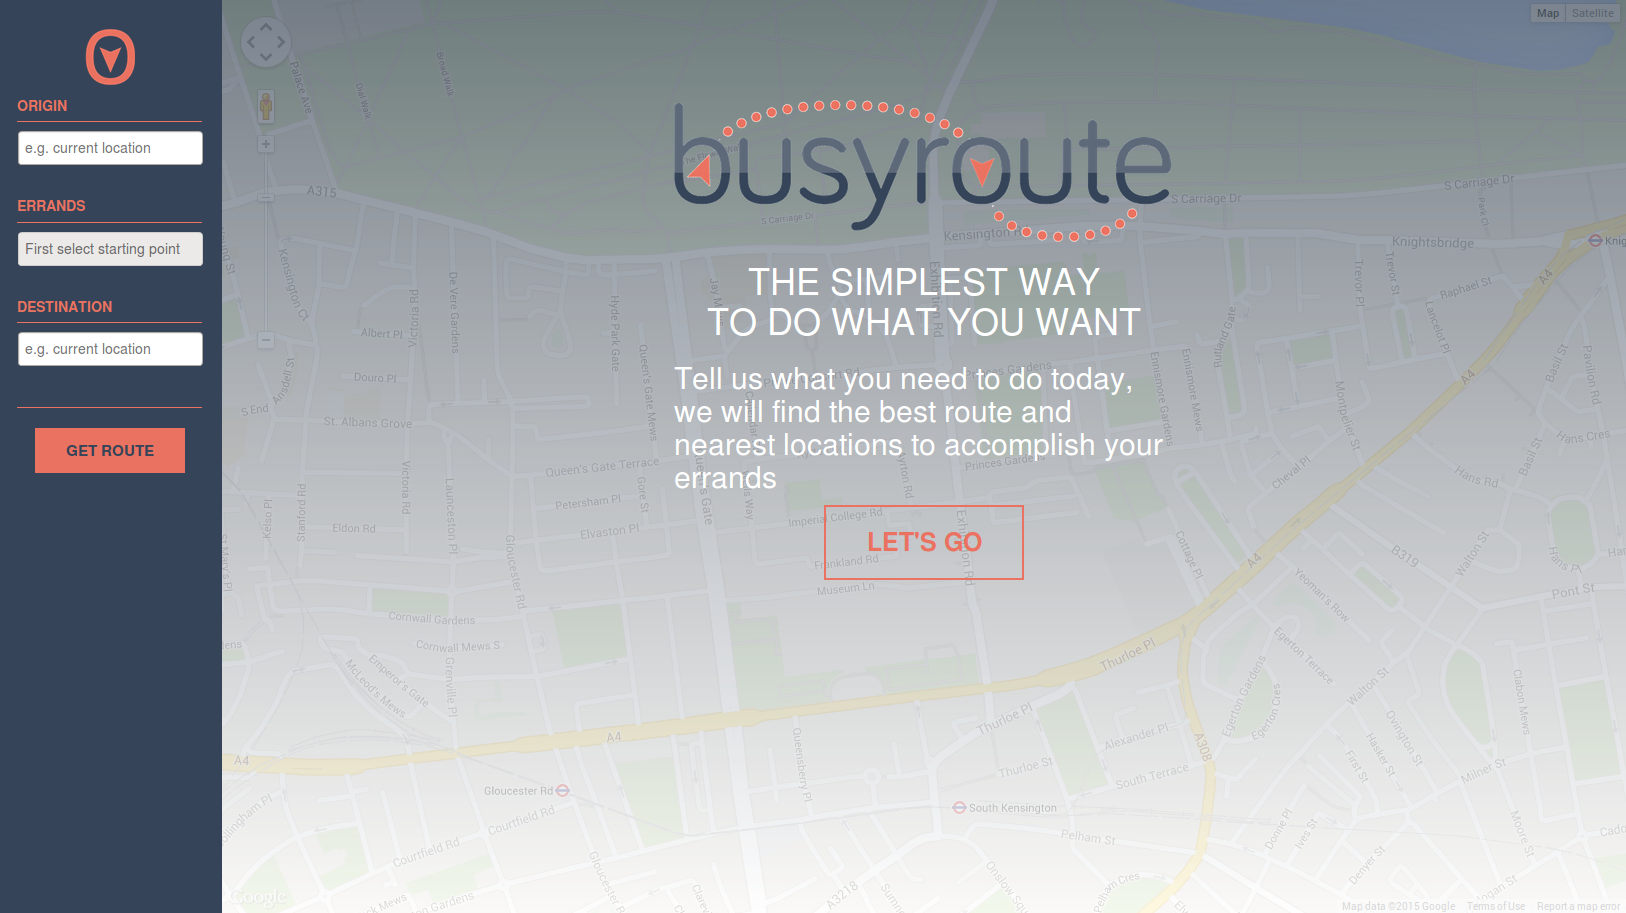
\includegraphics[scale=.13]{busyroute_landing.png}
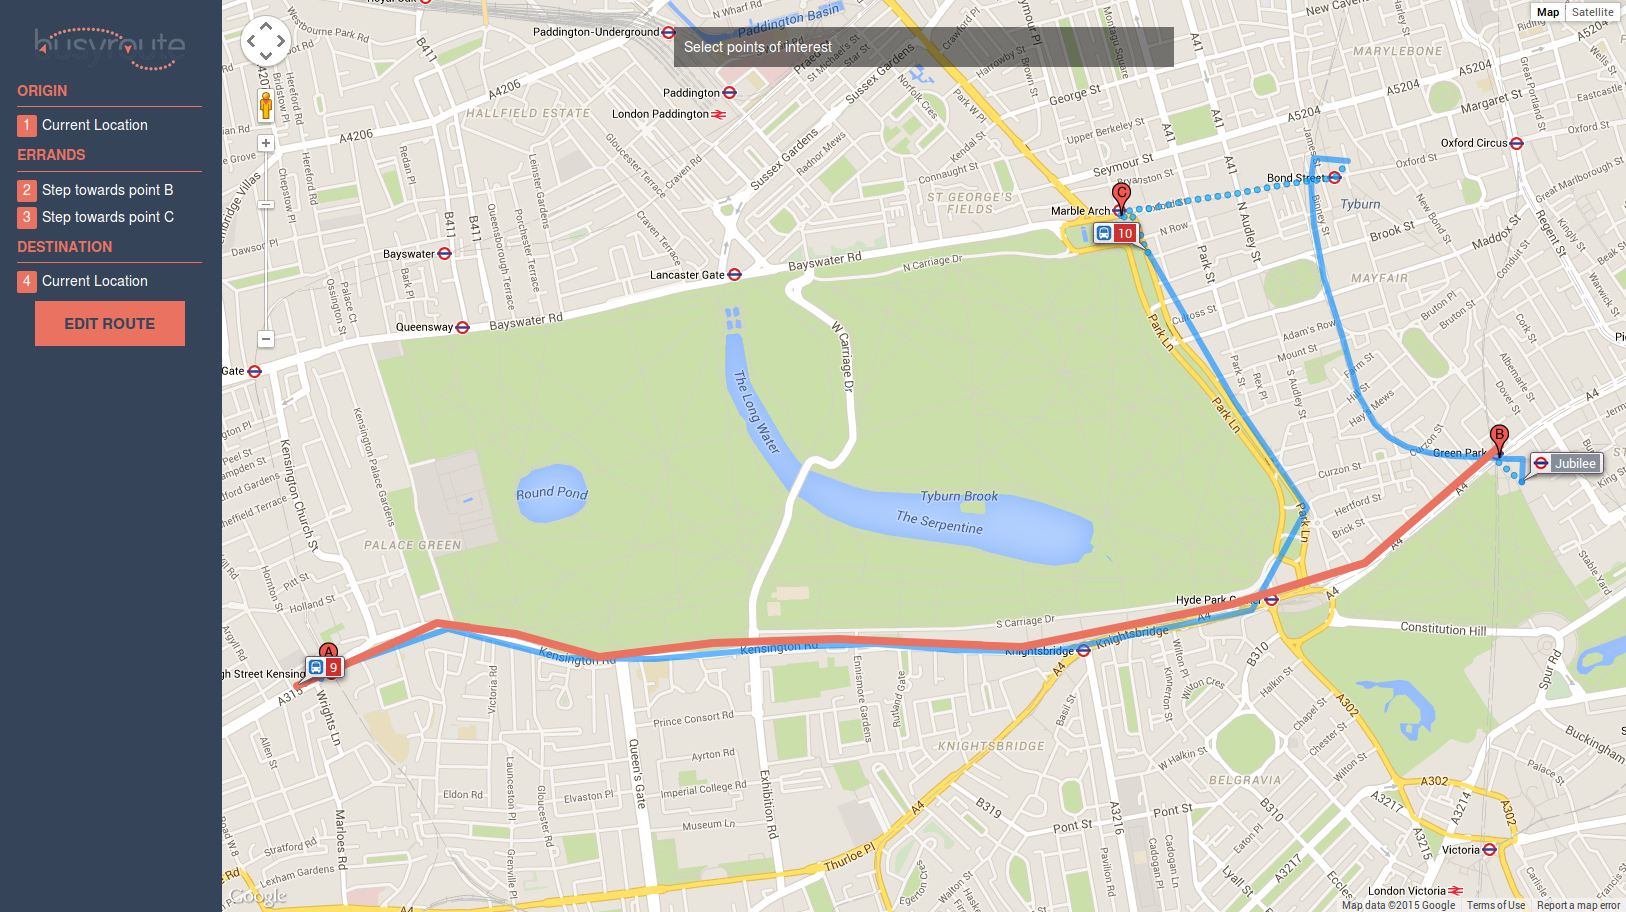
\includegraphics[scale=.13]{busyroute_route1.png}\\
Figure 1. Screenshot of our landing page and app in use.
\end{center}
Our project provides users with a system, named \textit{BusyRoute}, that can determine a suitable route to complete all of his/her tasks. This differs from existing routing products, as \textit{BusyRoute} is able to:
\begin{itemize}
\item cope with planning routes (using public transport) incorporating \textbf{multiple destinations}
\item in an \textbf{arbitrary order},
\item where the user might \textbf{not know the exact locations or types of locations} beforehand.
\end{itemize}
In motivation, consider a user who wants to post a letter and fetch a coffee, and is not overly concerned as to the specific locations where he accomplishes these tasks. \textit{BusyRoute} could suggest visiting a postbox the user is unaware of in a street closely neighbouring a nearby Starbucks store, rather than venturing to the Post Office he is familiar with, situated farther away; other routing solutions would not work since the user was unaware of the postbox, or would not be as efficient since the user would need to first learn that said nearby postbox exists.

\section{Achievements}
We are fairly satisfied that our application successfully implements all of the essential functionality discussed in section 2.2 -- for more details on how these were implemented, please consult chapter 4.
\begin{enumerate}
\item Our front-end allows users to specify tasks from a predefined selection (including buying coffee and doing laundry).
\item The web UI is easy to use; users type in what they want to do and we match this to possible tasks.
\item We have found ways to match user tasks to possible locations where users can complete their tasks.
\item Users can indeed select specific locations to include in the route.
\item Routes computed seem reasonable, if not optimal, especially when the number of points is small (in particular, when $n \leq 8$).
\item Our algorithm does successfully consider and utilise the Tube network, where appropriate.
\item Our algorithm is fairly fast; requests at our server are typically serviced within 1 second.
\item The output of our algorithm is presented to the user through the Google Maps API.
\end{enumerate}
Through the use of hallway tests and acceptance checks, we gather that \textit{BusyRoute} does indeed make planning easier, allowing our busy users to devote more of their time and energy towards actually getting their tasks done as opposed to simply planning. \textit{BusyRoute} also improves the efficiency and quality of users' plans, incorporating locations that users may not have thought of and choosing efficient routes, especially in situations where the best route is non-obvious. This will be discussed in greater detail in our analysis of the feedback we have received and our evaluation of our product, in chapters 5 and 6.\\
\\
One stretch goal which we did consider and eventually implement was offering users the option to have the precise locations to complete an errand selected for them. This entails solving the Generalised Travelling Salesman Problem (GTSP), the implementation of which is discussed in section 4.5.6.

\chapter{Project Management}
\section{Choice of Agile Methods}
In an age where consumers are becoming increasingly dependent on technology to solve many of life's (ever evolving) problems, it is vital that technology firms work in ways which allow them to be responsive to new and changing requirements. As a team working to design and build a product to a customer's specification, we identify a need to work in similar ways. Furthermore, as a team of full-time students with a very limited timescale, we see it of paramount importance to be able to work responsively, remaining flexible to allow for the inevitable maturation of our initially vague project brief.\\\\
Several members of our team have past experience with Agile and/or iterative development, largely through the course of summer internships and placements. In particular, we appreciated the merit of iteratively releasing our work; this allowed us to both refine our product to better meet the requirements of our customers (or managers in certain cases), as well as better gauge the scope of what we could do given a tightly-defined deadline.\\\\
We discussed several possible project and/or engineering management practices from various Agile development approaches (such as Scrum, Extreme Programming (XP) and Kanban), and considered their suitability bearing in mind our team's specific needs. We found that not all of these industry `best practices' as written are suitable for us -- to some extent, this is because we are currently students (and not software engineers in industry). We have to attend potentially up to 8 hours of lectures per day, and complete other coursework and assignments in parallel with this project. Thus, for example, daily standup meetings would not be practical since we might not necessarily be able to work on the project everyday. Furthermore, we have a very full aggregate timetable; as a result, the time we can meet as a team is severely constrained as well. Consequently, many of these `best practices' need to be adapted or modified to make them suitable for our working style.\\\\
During a summer internship, one team member gained exposure to Kanban processes. Working in a team which took such approaches to development, he was able to identify some of the ways in which they work well, but also how they could fail when applied to certain types of work. It was observed that, when working on operational tasks (such as bug fixing, small feature enhancements, etc.), limiting the number of tasks in progress and maintaining a prioritised backlog worked well; working in this way allowed for a continuous flow at a high velocity. During the placement the team switched to working on a larger 3-month project, where they were building an entirely new system from the ground up. Not changing the choice of Agile methods (for example switching to Scrum) soon proved to be problematic. With a new large project came many unknowns, and the lack of scheduled planning meetings and customer demonstrations soon resulted in a number of completed tasks needing respecification and thus reimplementation, leaving the team unable to push out new features at the rate at which they were able to when working operationally. As a team also working on an entirely new product, we feel that Kanban is too loose, and favour methodologies where planning meetings, demonstrations and timeboxed iteration periods are of high importance.\\\\
After much deliberation, we decided to adopt several project management practices from Scrum, as well as some of the engineering processes from XP. These practices, and our motivations for adopting them, will be discussed in the following sections.
\section{Project Management Practices}
We were unanimous in the belief that the approach we took to project management will have huge influence on our success. Working with a fairly large team (compared to projects of previous years) and a limited timescale to produce a  substantial product, we realised that without placing importance on the management of our work but simply the engineering practices we adopt, we would risk a slow velocity and thus potentially not completing an application which satisfies all of our customer's requirements.\\\\
We decided to adopt some of the practices of Scrum to manage how we work. We appreciate how well Scrum can work in industry; however, we have chosen to adapt some principles somewhat to better suit our (busy, student) team -- such as how we approach our Sprint Backlog (sections 3.2.1, 3.2.6).\\\\
Some of the team have experience in working with Scrum through summer internships, and were also thus able to share their views on which practices may or may not work for us. We thus decided to adopt the following practices.
\subsection{Sprints}
\begin{center}
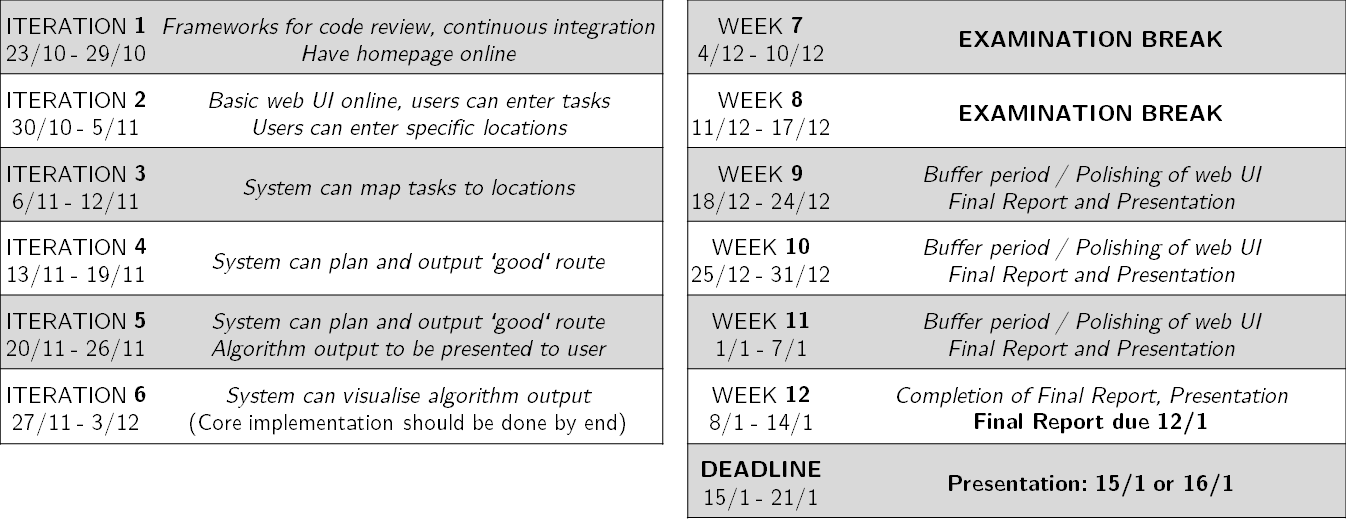
\includegraphics[scale=0.7]{release_plan.png}\\
Figure 2. Release plan showing initial iteration plans.
\end{center}
we worked through 1-week Sprint cycles. In industry, these cycles often last between 2 and 4 weeks (admittedly with a recent decreasing trend) \cite{sprint-len}, however with a timescale of only 6 weeks to complete the core implementation of our project, we identified that this would leave us having only 3 iterations and thus insufficient opportunity for feedback/requirement adaptation -- a poor granularity \cite{sprint-small-gd}. Also, short cycles helped us to make better use of information and feedback we could gather about our progress and velocity.\\\\
We held Sprint planning meetings at the beginning of each cycle, where we analysed and broke down high-level stories from the top of our prioritised (Product) ``Backlog". Though the PS is acting as our customer/product owner, she could not be in attendance at these meetings due to her busy academic schedule; however, all team members were present. All tasks we decided to commit to the upcoming Sprint were then placed in the ``To-Do" (Sprint Backlog) column on our storyboard (see section 3.4.1 for details). As is traditional, we approached the Product Backlog in a strict priority fashion \cite{sprint-backlog}. However, we also approach our Sprint Backlog in a similar way. We learnt that Scrum teams typically allow for more freedom as to the ordering of task completion mid-Sprint \cite{sprint-middle}, however in preparation for the possibility of not completing all tasks in a Sprint we chose to encourage -- where reasonable -- a somewhat stricter approach, to guarantee the completion only of the highest priority tasks.
\subsection{Velocity Measurement}
We used velocity measurement as a way of planning realistic and achievable Sprints. Tasks were given point scores after estimation, and the number of points of tasks completed from one Sprint helped us to more accurately predict how many pointed tasks should be included in the next.

\subsection{Demonstrations}
We met with our PS for one hour every week -- this was typically scheduled every Thursday at 11am. We used this time to showcase our latest work and gather as much feedback as possible. In addition, we also discussed the upcoming Sprint so that any features that the PS feels are of higher priority are brought to the top of our (Product) ``Backlog", ready for the subsequent Sprint planning meeting.

\subsection{Retrospectives}
We held short retrospectives after each Sprint to discuss our teamwork and assess how well our practices are working. Since our Sprints were relatively short, we were generally able to complete this in 10-15 minutes before we began to plan the following Sprint. We struggled to find any more time in our aggregate timetable to allow for a longer meeting; however, this time was generally sufficient and team members were able to express their concerns and/or satisfaction concerning the team's workflow.

\subsection{Scrum Master}
We chose to elect Thomas as the Scrum Master (SM) to act as team lead. Unlike traditional Scrum however, due to the nature of our team the SM also served as a developer. Our SM had the following three responsibilities \cite{scrum-master}, additional to his development roles:
\begin{enumerate}
\item Remove impediments that are obstructing the team's work. For example, if the team require additional resources or support with any tasks, the SM will identify what can be done to resume progress.
\item Own the success of the team's progress. This involves ensuring all deadlines are met and planned for accordingly, as well as making sure that the highest priority tasks as identified with the PS are planned for in the next Sprint. Additionally, the SM will pay close attention to the progression of each task mid-Sprint, and identify any bottlenecks. Frequent communication within the team will be encouraged by the SM.
\item Provide a point of communication between all parties. The SM will own all communication between the team and the PS, for example if additional meetings need to be scheduled.
\end{enumerate}

\subsection{Scrum vs. XP}
We considered project management practices from Scrum and XP. A key of the latter is that of shared understanding. We ensured that all team members are aware of one another's progress (through means discussed in section 3.4), and hence the progress of the team as a whole.\\\\
One key comparison we feel important to make is how Scrum and XP approach task prioritisation. In Scrum, the team can choose the order of completion of tasks from the Sprint Backlog. Contrastingly, XP enforces that all tasks (even at this low level) are completed in a strict priority order \cite{xp-scrum-diff}. As discussed, we will approach Sprint Backlog (in our case ``To-Do") tasks in a priority order similar to XP where possible. However, due to our individual timetables being filled with many other commitments including lectures, societies and sports, we will not enforce this policy as strictly as XP does. In many cases, we have a short period of free time (say 2 hours) on one day, and a longer period (say 5 hours) the following day. In these cases, we feel it makes far more sense to complete a shorter task first (since this could be completed in the 2 hour slot), even if it were of a lower priority to a longer task.

\section{Development Processes and Tools}
We analysed our development processes carefully -- with very limited time and resources, we needed to ensure that the code we produced was correct, and reasonable in terms of design and clarity. We thus developed a workflow which developers working on changes would go through -- this may be illustrated by Figure 3. We decided to adopt some of the software engineering practices espoused by XP, as well as include practices which we felt appropriate based on our (admittedly limited) experience in industry.
\begin{center}
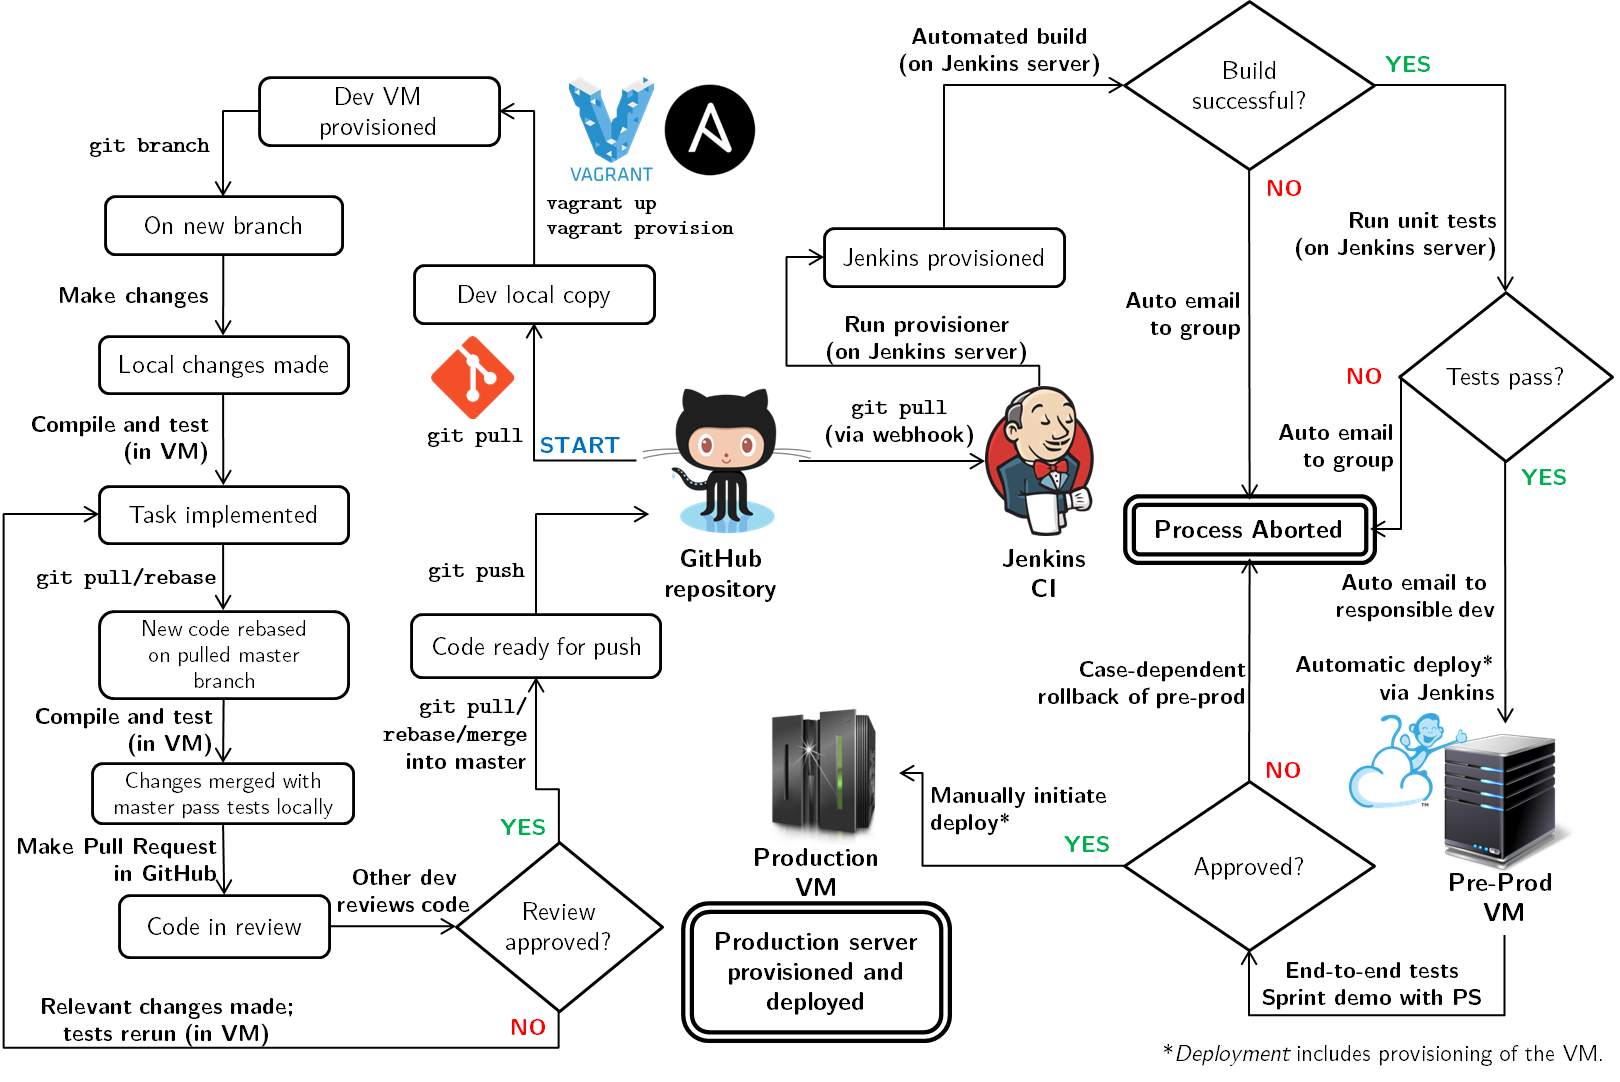
\includegraphics[scale=0.6]{workflow_diagram.png}
Figure 3. Diagram depicting our team's development processes.
\end{center}
\subsection{Git and Version Control}
We used \textit{git} \cite{git} for version control, and maintained a private \textit{GitHub} \cite{github} repository. This allowed us to create multiple branches for the features we are working on and ensure that the master branch always has a stable working version. Branches generally corresponded to ``In Progress" tasks; in order to ensure that individuals do not have too many branches and/or branches that last for a long time, we split our tasks into manageable subtasks (during our weekly planning meetings) and continuously integrated them into the main trunk. In order to maintain a clean and concise log on our master branch, we used Git's \texttt{rebase} and its interactive mode (\texttt{rebase -i}) to only keep a single, well-documented commit on the master branch for each feature that is developed.\\\\
We chose to use git for source control for several reasons -- it is free, sufficiently powerful for our needs (being able to create multiple independent branches) and is also the only tool that all team members were familiar with. As discussed in section 3.3.5, git and GitHub also readily interface with \textit{Jenkins} \cite{jenkins}, our choice of Continuous Integration server.
\subsection{Vagrant, Ansible and Development Environments}
We typically work on different operating systems (Linux, OS X and Windows) and in environments with different tools and utilities installed. Thus, in order to standardise our development and production environments (to avoid issues with code working in a developer's local environment but not in production), we used \textit{Vagrant} \cite{vagrant} a tool that sets up a standardised Ubuntu VM on the developer's machine. We used Vagrant together with \textit{Ansible} \cite{ansible}, a configuration management tool which allows us to specify ``playbooks" indicating, among other things, the software and services (such as the GNU C++ compiler or NodeJS) that our application requires. \\\\
Compared to other configuration management tools such as \textit{Puppet} \cite{puppet} or \textit{Chef} \cite{chef}, we found that Ansible had a much more forgiving learning curve. This was important due to our tight deadline; we did not want to spend too much time on figuring out how to implement server setup. Furthermore, while Puppet and Chef are more established and have larger communities, many of our requirements simply involved specifying that certain programs needed to be installed; what Ansible could do certainly satisfies our use-case.
\subsection{Test-Driven Development}
In order to minimise time spent debugging, reduce defects and gain assurance in the quality of our code \cite{tdd}, we have decided to require code to have unit tests and be green before submission. We also have several integration tests that check the interaction between various components in our system. This was accomplished using the \textit{GoogleTest} \cite{googletest} and \textit{Mocha} \cite{mocha} frameworks for C++ and JavaScript tests, respectively, and is discussed in greater detail in chapter 5. This gave us confidence in the correctness of our code and helped us more easily identify changes that might have caused a build to fail.
\subsection{Code Reviews}
We considered the possibility of using pair programming, a common technique used by XP teams. Working together when writing code helps to improve code quality and ensures that multiple team members will understand each individual piece of code. \cite{pair-program} That said, we acknowledged that this may not always be appropriate, for two reasons: \begin{itemize}
\item Team members have different individual schedules, and thus \textit{only} doing pair programming will severely limit the amount of development time available. 
\item In certain cases, we may wish to experiment with certain algorithms or features that may or may not make it to production; always requiring another team member to work on this may be inefficient.
\end{itemize}
We decided that Pair Programming may not be appropriate for our particular group. However, we wanted to keep code quality as well as our Bus Factor\footnote{the number of developers without whom we cannot proceed} high. We achieved this through a code review system -- when a task has been \textit{fully} implemented, it is required that at least one other member in the group approves the changes. To facilitate this, we made use of GitHub Pull Requests \cite{github-pull-req}; this helped us easily keep track of  communication regarding a review and updates made in response to feedback. 
\begin{center}
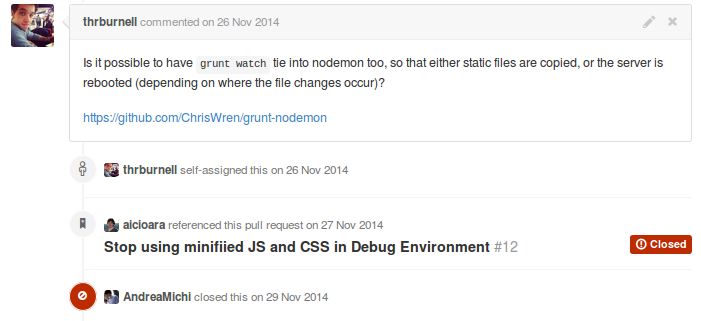
\includegraphics[scale=0.42]{pullreq.png}\\
Figure 4. A typical Pull Request undergoing review.
\end{center}
We were thus able to increase the number of people that are aware of each portion of the code, while not requiring two developers to be available to work on the project at the same time. Since reviews were only required when changes were merged into master, developers are free to carry out experiments or technical spikes on their own. However, a drawback of this system was that there were occasions when the code review process did slow down workflows especially when developers had many competing deadlines (from coursework or placement interviews).
\subsection{Demo Environments}
To help with the code review process, we set up demo environments; these environments run on a separate CloudStack server hosted by DoC. Pushing on their demo environment branch, each member can quickly show to the rest of the team any front-end features or changes they might have developed. Typically, code reviews especially for changes on the front-end would include a link to a demo environment with the relevant change included, allowing team members to easily have a visual overview of the changes.
\subsection{Jenkins and Continuous Integration}
\begin{center}
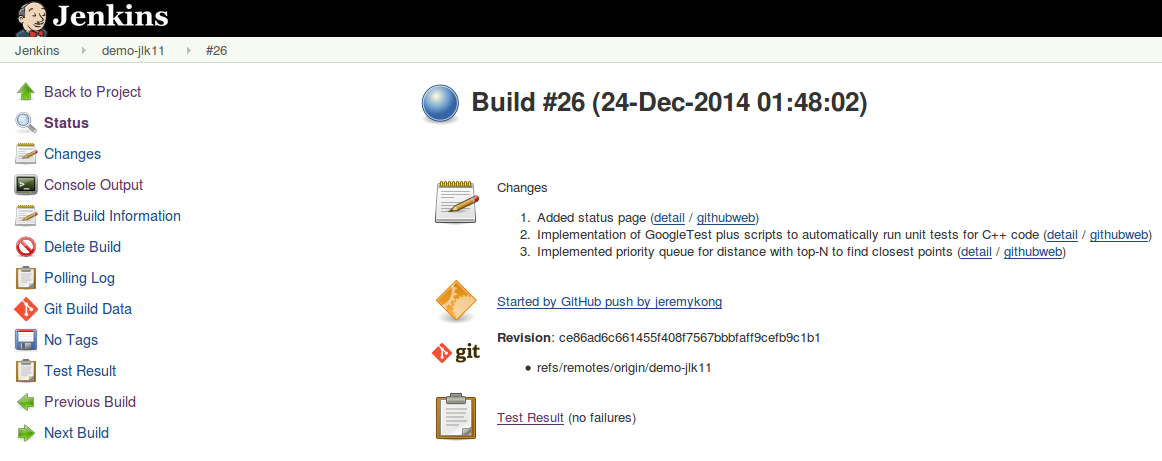
\includegraphics[scale=0.36]{jenkins_build.png}\\
Figure 5. Automated build on Jenkins server caused by a GitHub push.
\end{center}
We applied Continuous Integration practices described in the Software Engineering (Practice) course, to avoid the length and unpredictability of integrating potentially conflicting code \cite{ci}.
We used the \textit{Jenkins} \cite{jenkins} build system for continuous integration, as there was significant community support available as well as many plugins that we could use to help us accomplish what we wanted. 
\\\\Whenever code was pushed to the master branch of the central repository, Jenkins' \textit{GitHub plugin} \cite{jenkins-github-plugin} would automatically initiate a build on the Jenkins continuous integration server -- this would entail running our provisioner, Ansible, to set up the server, building our code and then running our suite of unit tests. In the event that the build is unsuccessful or tests do not pass, an email is automatically sent out to all developers, and the change is not pushed out further.
\subsection{Pre-Production and Production Servers}
In the event that the build is successful and all tests pass, Jenkins deploys our code to a pre-production environment. This allows us to perform manual user acceptance tests, as well as demonstrate the current state of our work to our PS.
\\\\
We opted for this approach instead of directly deploying to production, as there are several behaviours (for example, front-end graphical issues) that may be difficult or cumbersome for our unit and/or system tests to cover. Furthermore, we would sometimes want to seek approval from our PS before deploying our latest work to production; having a pre-production environment allows us to easily do this.
\\\\
From the pre-production environment, if we are satisfied that the system works as intended and the PS is also satisfied, we would then deploy our software to production. This can be performed by initiating a shell-script from the repository on the production server.
\section{Group Communication}
We agreed that clear communication was paramount in optimising our efficiency as a team. While face-to-face communication is effective, it is not always practical due to individual developers' schedules. We thus employed several tools in remotely communicating the state of our work to one another.
\subsection{Task Boards and Trello}
We identified early on that we wanted to be able to track our progress carefully -- we would like for all team members to be able to easily and quickly visualise all past, present and future tasks. In order to facilitate this, we took inspiration from the common Agile practice of utilising a columned storyboard, where task cards can be moved between categories which clearly convey the current status of the task which they describe. \\\\
We opted for using the online project management application \textit{Trello} \cite{trello}. Trello allows users to create projects, and provides many options (e.g. labels, progress bars, member assignment and deadlines) which allow for a highly customised storyboard. Moreover, unlike other alternatives such as \textit{Jira Agile} \cite{jira} from Atlassian, Trello is free -- an undeniable advantage given that our project is not funded.
\begin{center}
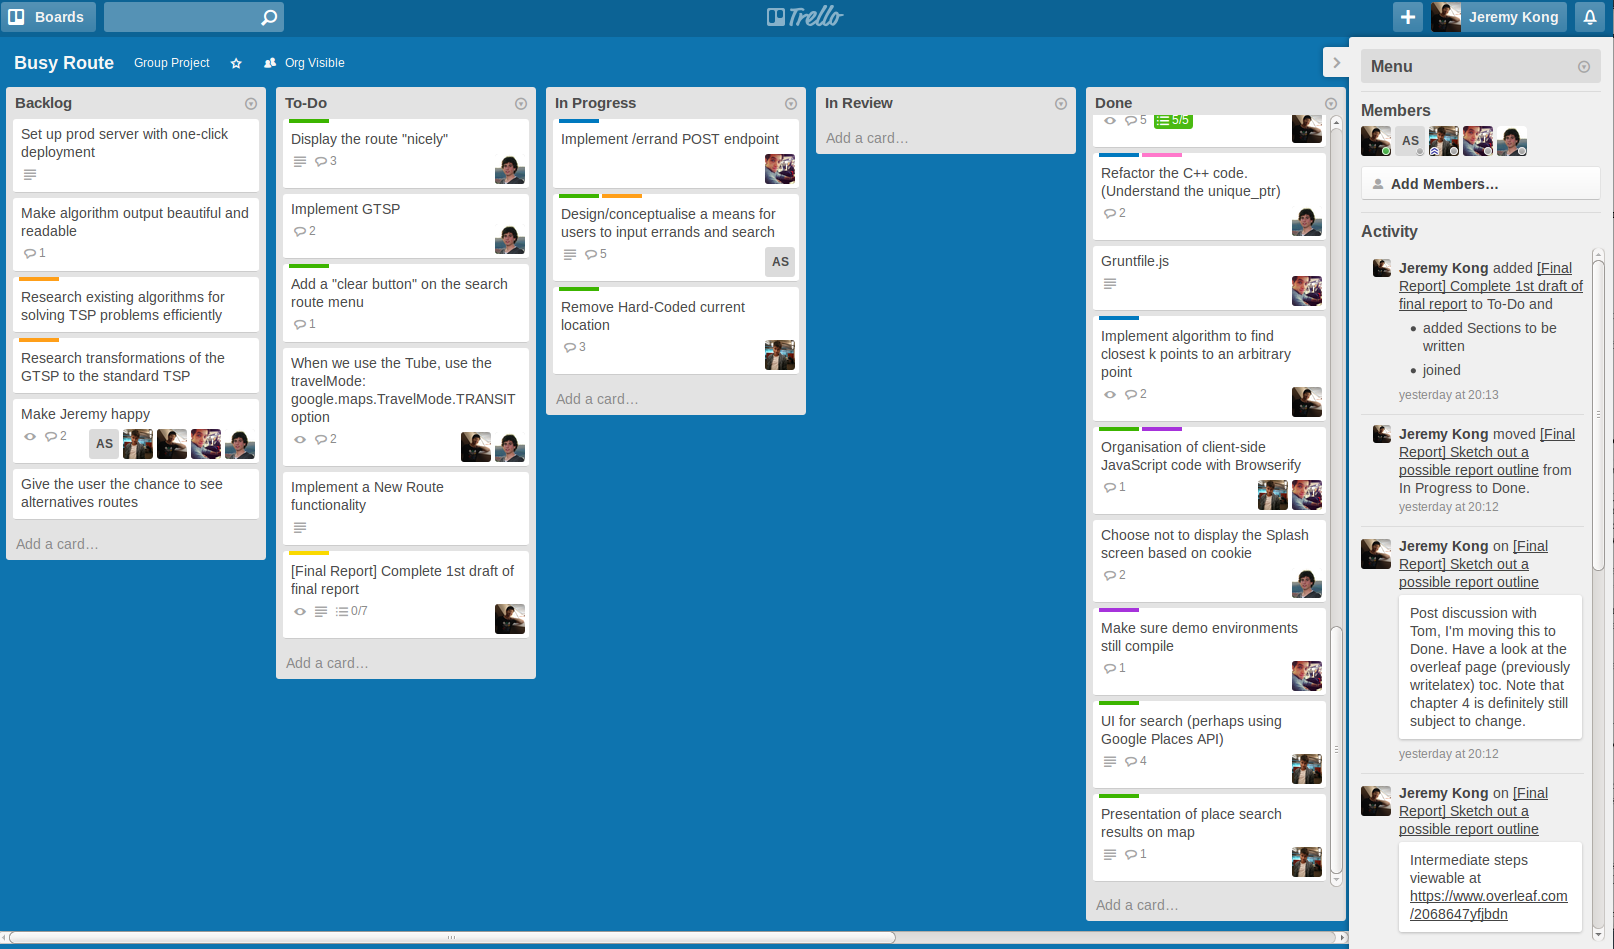
\includegraphics[scale=0.27]{trello.png}\\
Figure 6. Our group's Trello board.
\end{center}
Taking inspiration from lecture material and past internship experiences, we designed our storyboard with five main columns, described below from left to right:
\begin{itemize}
\item The \textbf{``Backlog"} column shows a list of high level requirements for our project. These requirements have not been analysed yet, so this column can be seen as a list of user stories documenting features desired by our customer.
\item The \textbf{``To-Do"} column contains tasks that have been analysed and estimated. This column is repopulated at the beginning of each Sprint during the Sprint planning meeting. We try to fill in this column with only as much as we estimate we can do throughout a Sprint.
\item The \textbf{``In Progress"} column refers to tasks which are currently under development. In practice, developers choose tasks from the ``To-Do" list and move them here. We keep this column as tidy as possible and aim to (generally) have at most one task per person; we find that focus is often lost when switching between task contexts.
\item The \textbf{``In Review"} column refers to tasks which have been finished, but have yet to be reviewed by another member of the group. Developers move their tasks here when they have submitted a Pull Request in accordance with section 3.3.4.
\item The \textbf{``Done"} column refers to tasks or features for which implementation has been completed, but have not yet been demoed to our customer. It also gives us a quick overview of what has been done during the current week -- tasks stay here until the following demo meeting, where features are presented to the PS and approval sought.
\end{itemize}
\subsection{Facebook Group}
%Sophia wants this.
\begin{center}
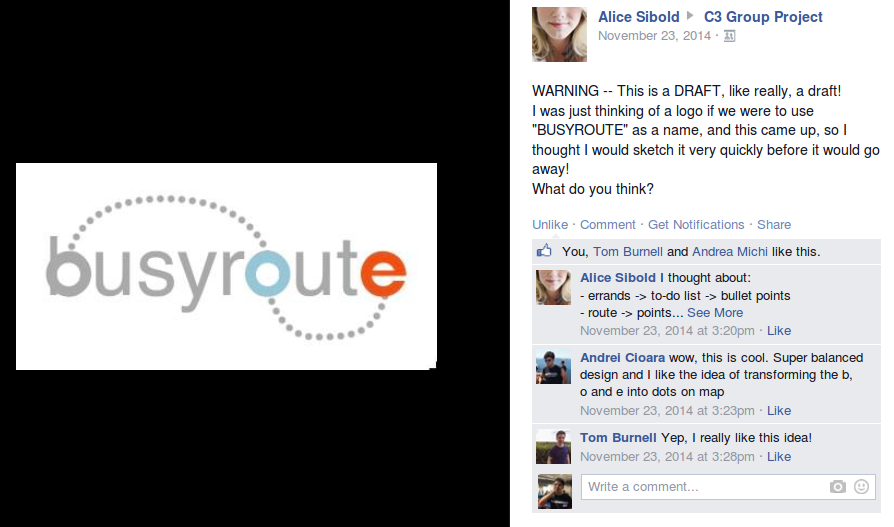
\includegraphics[scale=0.3]{facebook_communication.png}\\
Figure 7. Communication on our private Facebook group.
\end{center}
We used a private Facebook group for communication. This was the fastest way to broadcast a message as all group members use the platform regularly; some of us also receive Push Notifications to our mobile phones when a message or link is shared on the group.
\subsection{Google Drive}
In order to organise our non-code files (such as documentation), we needed a storage space easily accessible by all team members. File hosting services such as \textit{Dropbox} or \textit{Google Drive} offer the possibility of creating shared folders. We chose the latter over the former, since it allows concurrent editing and comments on documents. This makes remote reviewing of documentation by other team members easier.\\\\
Key files stored in our team's Drive include meeting minutes and design documents, as well as a Developer Handbook. The meeting minutes allow us to remind ourselves of what has been discussed during a meeting. Minutes are in point-form and tend to be small and concise, so they are also a good way of getting all the team members on the same page. This is especially relevant during meetings with our PS, where minutes taken become the basis of our Backlog items. The Developer Handbook contains guidelines that we agreed on concerning the use of developer tools such as git or Vagrant -- it served as a useful reference especially for team members who were less familiar with these tools.
\section{Group Organisation}
We did not initially allocate team members to specific tasks; originally, we intended for developers to select the highest priority item from the Sprint Backlog when done with their task (see section 3.2.1 for details). However, due to differing skill-sets and preferences, as well as the complexity of some of the problems encountered, team members soon ended up largely working on different parts of the system. These divisions were certainly not strict; team members would freely help one another where useful.
\begin{itemize}
\item \textbf{Thomas Burnell} was the team leader and Scrum Master (see section 3.2.5 for more details on this). He focused on developing and implementing our back-end algorithms for matching user errands to locations. Thomas was also in charge of setting up the demo environments (see section 3.3.5 for more details), which allowed us to review changes to our front-end more easily.
\item \textbf{Andrei Cioara} designed and implemented various strategies for solving (or approximately solving) the TSP on the back-end. He also worked on much of the routing logic involved in the communication between clients, our server and the services we are using (such as the Google Directions API). He was also in charge of preparing our hallway testing programme.
\item \textbf{Jeremy Kong} developed and implemented the heuristics used to estimate edge weights for the TSP on the back-end, bearing in mind usage restrictions from the various APIs we used; he also worked on solving the TSP. He also focused on the team's documentation, taking charge of preparing reports and coursework submissions as well as keeping track of group meetings.
\item \textbf{Andrea Michi} worked primarily on the front-end; he set up much of the JavaScript front-end, both in terms of accepting input from the user, as well as coordinating user requests and the relevant underlying API calls. Andrea also worked on designing and implementing the logic used to match errands to locations.
\item \textbf{Alice Sibold} focused primarily on the design and implementation of the front-end interface presented to the user, ensuring that it was simple and accessible to users yet sleek and elegant. She also developed paper prototypes and mock-ups throughout the project that allowed us to quickly gather user feedback concerning our user interface.
\end{itemize}

\chapter{Design and Implementation}
\section{Software Design / Architecture}
% No more layer diagram. We're assuming the design without GTSP.
We identified fairly early on that the architecture of our application \textit{could} be designed such that it is composed of three largely distinct components:
\begin{enumerate}
\item A \textbf{web interface}, which takes requests input by the user and sends it to the relevant underlying services, presenting their results back to the user.
\item A \textbf{location finder}, which given a specific errand such as ``getting a coffee" or ``visiting the gym" finds possible locations where said errand can be completed.
\item A \textbf{router}, that given a series of points, calculates an efficient route through the points in any order (possibly using public transport).
\end{enumerate}
Maintaining a modular design helps to reduce the rigidity, fragility and immobility of our code. \cite{separate-concerns} Keeping these components separate also allows for a greater scope of extension; separating out concerns into distinct interacting components will allow us to introduce additional functionality and features later down the line much more easily than if we were working in one monolithic codebase. \cite{separate-concerns-2}\\\\
Various design decisions were made however that resulted in a somewhat different -- yet still modular -- design. This may be best expressed through a systems map, as follows:
\begin{center}
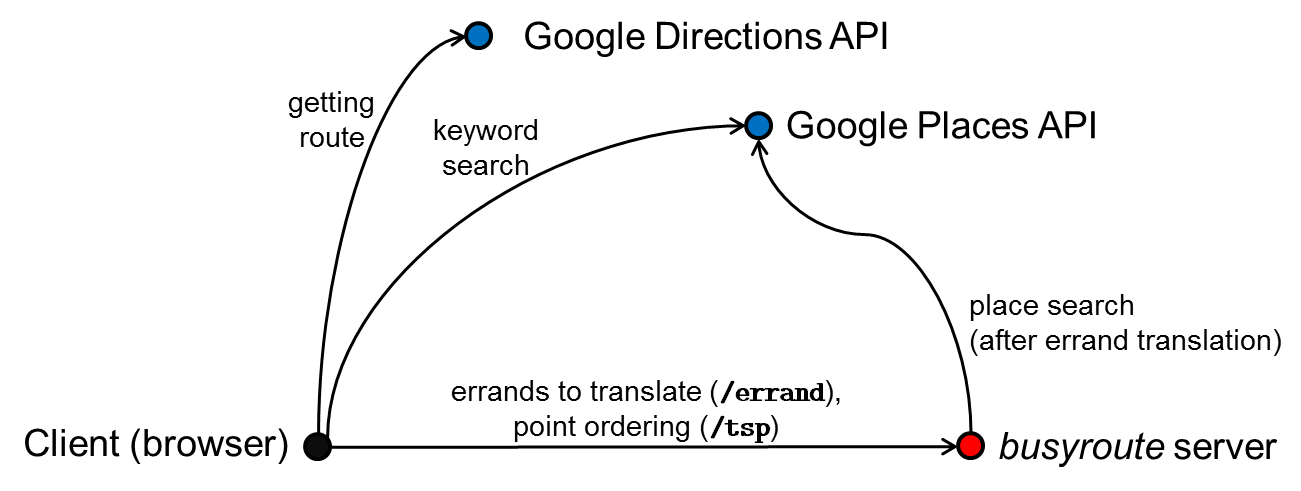
\includegraphics[scale=.6]{systems_map.png} \\
Figure 8. Systems map illustrating our system's architecture.
\end{center}
Our web interface provides to the user a way for inputting his errands. Calls are made to our server’s exposed \texttt{/errand} API, which returns a list of suitable places. These are presented to the user, allowing him to choose the place which he prefers. Once the user has finished selecting all the places he needs to visit, the client makes a series of API calls. The client first calls another internal API, \texttt{/tsp}, which performs preprocessing over the set of user-chosen points, returning to the client a permutation of the given points which is deemed as the solution to the TSP over said points. The client then makes calls to the Google Directions API \cite{google-directions}, for finding the exact route between each pair of adjacent points in the route. The Google Directions API returns routing data which is applied to the map canvas, thus displaying the route. \\\\
In addition to allowing users to find points by searching high-level errands, we allow for users to perform more specific keyword searches; the errand ``Get a light lunch" may be suitable for user Alice, however Bob’s appetite may be more restrictive and so a search for ``Wasabi in South Kensington" may be more helpful. Searches of this type are not handled by our server, but rather directly by Google Places. Unlike errand translation, direct queries like this require no preprocessing, and thus calling Google Places directly from the client -- instead of indirectly via our server -- avoids unprofitable additional network requests. \\\\
Design decisions were made that resulted in no closed router component \textit{as defined above} being part of our architecture. The logic for finding the ordering of user-selected points with minimal cost is housed in our server, exposed internally via the discussed \texttt{/tsp} API. Once this ordering has been computed however, routes between each pair of adjacent points are trivially found using the Google Maps API. Thus, with scalability in mind and in order to reduce server-side network overhead, we decided to place the responsibility of querying Google Maps for routes on the client.
\section{User Interface}
\subsection{Back-End Frameworks: NodeJS and ExpressJS}
We considered several possibilities for web development technologies that could be suitable for our back-end. All of these options have a fairly well-developed community and suitable frameworks which make them robust, scalable and fast. These options include \begin{itemize}
\item \textit{PHP} and the \textit{Laravel} \cite{laravel} framework
\item \textit{Ruby} and the \textit{Rails} \cite{rails} framework
\item \textit{Python} and the \textit{Django} \cite{django} framework
\item \textit{NodeJS} and the \textit{ExpressJS} \cite{expressjs} framework
\end{itemize}
We decided to use \textit{NodeJS}. Our server backend is neither particularly large nor overly complex; thus, all of the aforementioned options were feasible. The two main reasons for this decision were as follows:
\begin{itemize}
\item \textit{NodeJS} is becoming increasingly popular in the web development community \cite{nodejs-popular}; it is heavily used by small-medium enterprises in industry.
\item Team members were largely familiar with frontend JavaScript; thus, the overhead of learning \textit{NodeJS} would be minimal.
\end{itemize}
We chose \textit{ExpressJS} for our framework as it is very well-documented. We also considered not using an established framework; however this would complicate things as more components were added. Using \textit{ExpressJS} helped us reason more clearly about modularity within our project and separation of concerns (between the View and Controller). \textit{ExpressJS} also had ready support for our HTML templating engine, \textit{Handlebars} \cite{handlebars}, and our unit test framework, \textit{Mocha} \cite{mocha}.
\subsection{Front-End Frameworks: Browserify}
We have decided not to use a mature Front-End framework for our application. Some popular choices would have been \textit{AngularJS}, \textit{EmberJS}, \textit{KnockoutJS }or \textit{BackboneJS} \cite{js-frameworks}. These frameworks are all expressive and have well-established communities; however, they were not a good fit for the type of application we built. There was no need for us to have an MVC system in place, since the view is mostly generated by the backend. Also, most of our JavaScript code performs Google Maps API integration and/or map interactions, therefore vanilla JavaScript was sufficient.\\\\
After several iterations, we observed that our JavaScript frontend codebase grew bigger; it became harder to maintain and work with. We initially kept all of our JavaScript code in a single file, \texttt{app.js}; this soon proved difficult to manage. (We did this since spreading the code across multiple files made it inconvenient to reference code/functions across files.) \\\\
We decided to use \textit{Browserify} \cite{browserify} to solve this issue. We used the Module Pattern (very common in JavaScript) to separate our code into logical modules, each in its own file \cite{module-pattern}. The modules can then be referenced between files by using the \texttt{require} keyword. \textit{Browserify} takes all of the modules and compiles them together in a single, big JavaScript file, which is the file served to the browser. The generation of this file is performed at build time, initiated by the \textit{Grunt} Task Runner \cite{grunt}. We were thus able to preserve modularity and logical separation of tasks, while not losing performance on the browser side.
\subsection{Front-End Styling: SASS}
We have used \textit{SASS} \cite{sass} for styling our application; \textit{SASS} is a simple extension of CSS which allows us to use nesting and variables. We built our application with Software Engineering principles in mind and thus decided that using variables to factor out common attribute values would be a good practice, making future changes easier to perform. SCSS (``Sassy CSS") is the syntax we used for our SASS. This is basically a superset of CSS3's syntax, which means that every valid CSS stylesheet is valid SCSS. Thus, the overhead of using this technology was fairly minimal. 
\subsection{HTML Templating: Handlebars}
HTML templating is a technique used to reduce code duplication and improve readability of HTML; code written in a templating language compiles down to regular HTML. Typically, boilerplate (such as \texttt{<head>}, \texttt{<body>} tags, JavaScript \texttt{<script>} tags, closing tags, etc.) is automatically added. \\\\
Two popular templating engines we considered were \textit{Handlebars} \cite{handlebars} and \textit{Jade} \cite{jade}; an argument for \textit{Jade} was made on the basis that it is simpler to read and write. However, we decided to use \textit{Handlebars} as its syntax was more in line with HTML; Jade had a considerably different syntax from regular HTML and learning this would have presented an additional overhead. \\\\
\textit{Handlebars} allows us to generate pages dynamically; this can be used to send information from the back-end to the front-end. In our application, we need to send the encrypted Google Maps API key from the backend to the frontend; our provisioner \textit{Ansible} \cite{ansible} sets the value of a suitable environment variable (see section 3.3.2 for more details) on our server and this is sent to clients.
\subsection{Errand Input: Fuse.js}
\begin{center}
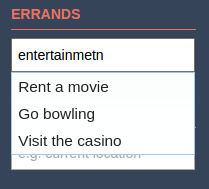
\includegraphics[scale=0.5]{fuzzy_search.png} \\
Figure 9. Matching (erroneous) user input to possible errands using approximate string matching.\\
Although the user has entered \texttt{entertainmetn}, we still list errands with keyword \texttt{entertainment}.
\end{center}
Our application allows users to type in a partial description of what they need to do. Our application will then suggest options through the jQuery-UI autocomplete widget \cite{jquery-autocomplete}.  \\\\ We have a predefined dictionary of errand types available; each errand is matched with certain keywords that users are likely to search for (for example, users seeking to grab a coffee might search for ``coffee", ``drink", or ``caffeine").
We perform approximate string-matching with the \textit{Fuse.js} library; this allows us to cope with misspellings and typographical errors in user input (which the jQuery-UI widget does not support). \cite{fuse-js}
\subsection{Point Selection and Route Display: Google Maps}
\begin{center}
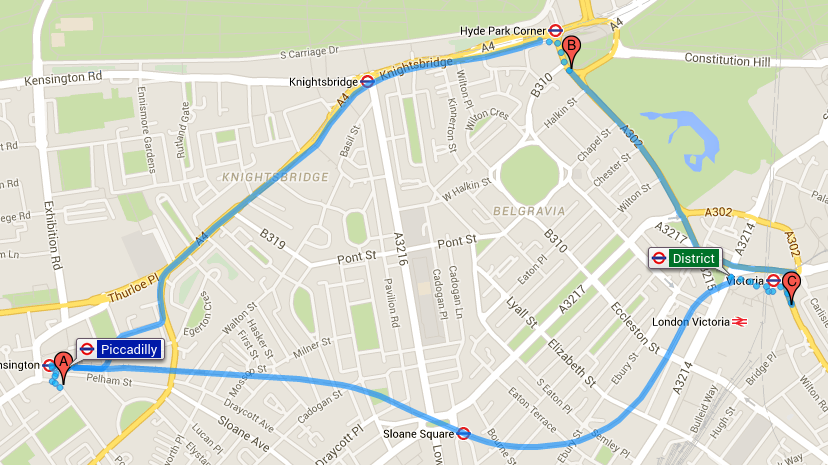
\includegraphics[scale=0.4]{gmaps_route.png} \\
Figure 10. Route display using \textit{Google Maps}, showing transit directions.
\end{center}
We are using the \textit{Google Maps} JavaScript API \cite{gmaps-js} for route visualisation. Users can select points and view the current state of their itinerary on the map; when users request a route from our application, this will be depicted graphically on the map, as well. \\\\
The strongest motivation for us choosing \textit{Google Maps} was that our customers were likely to have used it before and would thus find it comfortable and easy to use; our PS personally favoured the \textit{Google Maps} interface. The \textit{Google Maps} API also supported a simple and clear way for presenting transit directions to the user (as shown above), as compared to alternatives such as \textit{OpenStreetMap}. \cite{openstreetmap}
\subsection{Design and Artwork}
\begin{center}

\includegraphics[scale=.5]{busyroute_v7.png} \\
Figure 11. \textit{BusyRoute} logo.
\end{center}
We have designed our own logo and images for this project; apart from several images from Google Maps (such as the pins) that were chosen to be consistent with the rest of the Google Maps interface, all assets used were custom made.
\subsection{Internationalisation}
We have kept our product amenable to internationalisation, by ensuring that strings are externalised. All strings presented to the user have been extracted into a locals file and are referenced via an internal identifier, rather than including the string itself in our code. This makes our application adaptable for most other languages, as all we need to do is translate the locals file strings and use the appropriate locals file for the appropriate location. \cite{i18n}
\section{Mapping Errands to Locations}
Very early on in our project planning, we considered the feasibility of natural language processing, allowing users to type their errands as fluidly as ``I need to buy milk" or ``Pick up groceries". However, when sensibly assessing the scope of our project, we identified this was far outside. We thus decided to define a (fairly comprehensive) set of supported errands, which users could search through (using an intuitive fuzzy search as described in section 4.2.5).
\subsection{API: \texttt{/errand} endpoint}
The client offers the user a way for inputting errands, allowing him to search through our list of supported errands. When the user hits enter, a POST request is made to our server, at \texttt{/errand}. The request data is structured as follows:
\begin{verbatim}
{
    "errand": "buy_coffee",
    "areas": [
        {
            "location": {
                "lat": 0.1, "lng": 0.2
            },
            "radius": 600
        }
    ]
}
\end{verbatim}
In the structure above, errand corresponds to our application's unique identifier for the errand of interest. The given areas each contain location coordinates to search near, and an optional search radius (if not provided, the API defaults to 500). The example request above corresponds to the query ``find me all places where I can buy coffee, that are within 600m of point (0.1, 0.2)". This API is designed so that errand locations are searched for near all of the currently user-selected points. To clarify, if a user has already selected the Starbucks store to grab a coffee at and the ATM at which to withdraw cash, then should he search for somewhere to do his laundry, he will be presented with suitable locations near his starting position, and the Starbucks store and the ATM.\\\\
The client receives as a response an array of place objects, which are defined as per Google's \textit{Places API} \cite{google-places}. The client interprets them as such, thus being able to easily place corresponding pins on the map canvas.
\subsection{Supported Errands}
The errands our application supports are defined in the file errand-definitions.json. The file is structured as such:
\begin{verbatim}
{
    "buy_coffee": {
        "colloquial": "Grab a coffee",
        "search_keywords": ["coffee", "caffeine", "hot drink"],
        "googleAttributes": {
            "types": ["cafe"],
            "keyword": "coffee"
        }
    },
    ...
}
\end{verbatim}
An errand is indexed by a unique identifier; in the example above, ``buy\_coffee" represents the errand that, to the user, is presented as ``Grab a coffee". The \texttt{search\_keywords} provides an array of key words which, when searched by the user, should match against this errand. The remaining attributes are used for Google Places requests, as discussed below.
\\\\
In order to keep the client aware of all supported errands, our build system generates a static JSON file from the \texttt{errand-definitions.json} config. The generated file is served to the client, including all the colloquial representations with corresponding search keywords and API identifiers. This allows us to define new errands easily by making a change to one file, and deploying.

\subsection{Google Places}
We make use of the \textit{Google Places API} \cite{google-places} for finding places suitable for completing errands. Google's API allows for places to be searched for by a number of different arguments, including keyword, place name, price range, etc. An additional way of querying is by place type, where type is one of the many Google-defined place types \cite{google-places-types}. Each errand, as shown in the config above, has an associated set of attributes that are required to be sent with each related Google Places query. For example, the ``Grab a coffee" errand requires keyword ``coffee" and type ``cafe", whereas ``Buy some groceries" requires the types ``groceries", ``food" and ``supermarket" only.
\\\\
With each Google Places query, we also specify a vicinity to search within. For each of the client-specified areas (refer to API section), a corresponding query is made. The union of all associated responses is returned to the client.
\subsection{Specific Place Search}
We identified a need for search functionality outside of our supported list of errands. There are a couple of motivating reasons for this: firstly, we would like the user to be able to find a place to complete an errand that is not supported by our list; secondly, we would like the user to be able to find a more specific place to complete an errand that may already be supported (for example, ``Starbucks", vs. ``Grab a coffee", may be a more suitable search query for one who favours commercialism over quality of coffee bean roast\footnote{Purely subjective, of course.}).
\\\\
Searches of this type are performed by keyword, and are sent from client to Google Places directly, rather than via the server (since no translation preprocessing is required).
\section{Modelling Edge Weights}
The calculation of the time required to travel from point $A$ to point $B$ while possibly using public transport proved to be a nontrivial task. 
\subsection{Problems with Using External Services}
We first considered the possibility of delegating this operation to an external service -- this is supported by \textit{Google Maps} \cite{google-maps} as well as the Transport for London \textit{Journey Planner} \cite{tfl-journey-planner}. However, this quickly proved infeasible -- for a single request to our server containing $N$ errands, we determined that we would need to make $(N + 1)^2 - (N + 1) = N^2 + N$ API calls to determine the travel times between each pair of locations. (Note that travel times between points can often be asymmetric.) For example, Google Maps does have, for free services, a usage limit of $2,500$ requests per day -- if an average request has just $6$ errands, that restricts our server to $\lfloor \frac{2500}{42} \rfloor = 59$ requests per day\footnote{Even less, actually, since larger requests require quadratically more API calls.}. In any case, this would also introduce a significant amount of network overhead, increasing service time; this would be undesirable, seeing as one of our goals was that our application be convenient to use.
\subsection{Modelling Public Transport Networks: Design}
We thus needed to develop an internal model that could determine how public transport could be used to travel between locations. We discussed with our PS and agreed that for the scope of this project, it would be sufficient to incorporate support for just London Underground. However, in order to maintain scope for extension of this to other public transport services (perhaps in London, such as the DLR or Overground; or even in other cities), we had to design how we modelled the Tube network carefully. \\\\
We designed several collaborating classes in C++, as follows:
\begin{center}
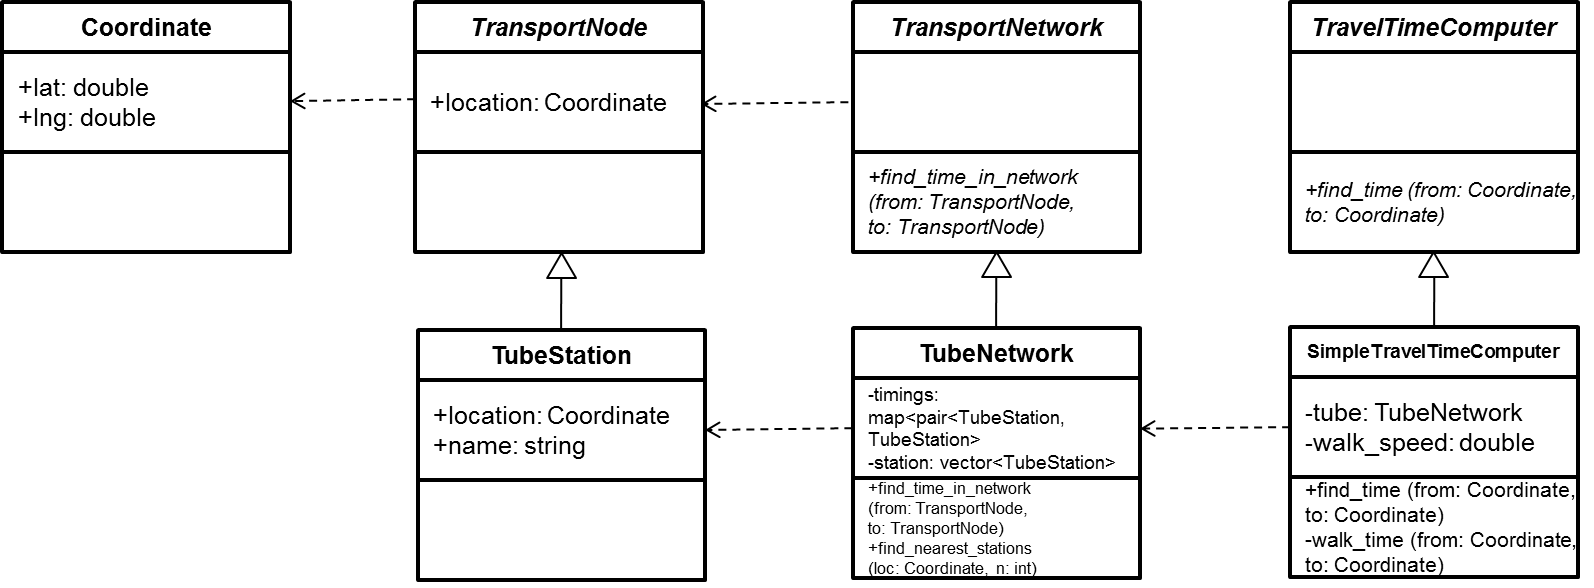
\includegraphics[scale=0.6]{uml_tube.png}\\
Figure 12. UML Class Diagram of Tube-related classes
\end{center}
\begin{itemize}
\item A \texttt{Coordinate} models a point on the Earth's surface -- its latitude and longitude.
\item A \texttt{TransportNode} models a station on a transport network. It stores a \texttt{Coordinate} object (though their behaviour could be extended, perhaps with opening hours). 
\item A \texttt{TransportNetwork} (abstract class) typically works with \texttt{TransportNode}s and has a (pure virtual) \texttt{find\_time()} method. This takes two \texttt{TransportNode}s and determines the time taken to travel from the first to the second, strictly via the transport network being modelled.
\item A \texttt{TubeNetwork} models the London Underground network.
\item A \texttt{TravelTimeComputer} (abstract class) has a (pure virtual) \texttt{find\_time()} method, which takes two \texttt{Coordinate}s and returns the time required to travel from the first to the second. We expect that implementations of this class are likely to make use of \texttt{TransportNetwork}s by composition. The \texttt{MapPoints} class uses the Strategy Pattern with this class when determining edge weights.
\item A \texttt{SimpleTravelTimeComputer} is the concrete implementation of \texttt{TravelTimeComputer} we use. This currently supports both walking and taking the Tube (hence it uses a \texttt{TubeNetwork}).
\end{itemize}
Implementing our model in this way would allow for easy addition of more \texttt{TransportNetwork}s (such as a \texttt{BusNetwork} or \texttt{RailNetwork}) and have their behaviour handled by a \texttt{TravelTimeComputer} -- a first step could be to simply select the individual network giving the fastest routes. A possible issue with this design might be handling transfers between different public transport networks (which may be part of an optimal / efficient route), though implementations of \texttt{TimeTravelComputer} may be able to intelligently coordinate requests to the underlying \texttt{TransportNetwork}s.

\subsection{Building the \texttt{TubeNetwork}}
We similarly considered delegating finding the time between each pair of stations to external services, by making requests to the relevant API. However, this quickly proved difficult as there are $270$ stations on London Underground \cite{tube-stat}, and hence we would need a total of $270 \times 269 = 72,630$ requests. Using the Google Maps APIs this would require 30 days of queries; while Transport for London's Journey Planner API does have a higher usage limit of 300 requests per minute, and 4 hours is an acceptable cost for a highly infrequent operation, using the API requires IP whitelisting; while our group did apply for this, it took several weeks for approval, which was an unacceptable delay. \\\\
When travelling from station $A$ to station $B$ on the Tube, several factors need to be considered:
\begin{enumerate}
\item Time spent walking from the turnstiles to the platform at the origin.
\item Time spent waiting for train(s).
\item Time spent travelling in train(s).
\item If changing trains, time spent walking from one platform to another at the relevant interchange.
\item Time spent walking from the platform to the turnstiles at the destination.
\item Service delays and disruptions.
\end{enumerate}
Our internal model currently does not account for (6); this could be included in an extension if we had more time (data concerning the status of Tube lines could be periodically queried and cached on our server; the number of API calls would be largely independent of the volume of requests we receive). \\\\
Transport for London released much of the data relevant to (1), (4) and (5) after a Freedom of Information request made by a member of the public. \cite{foi-chris} Data concerning (2) and (3) was also available through working timetables released by Transport for London, for the various Tube lines. These timetables included data about the average period of trains as well as average time trains spend on each segment\footnote{A segment here refers to two stations on a line that are directly connected.} of their route. \cite{tfl-wtts} We acknowledge that our model simply uses an average figure for inter-train arrival times instead of being time-sensitive; as before, this could perhaps serve as scope for future extension. \\\\
We used this information to write a simulator, \texttt{tube\_network\_generator.cpp} that uses a best-first search algorithm to use the data to calculate the time required between a station and all other stations; by running it across each station we could then obtain the time required to travel between all pairs of stations. In particular, a challenge we had to deal with was that edge weights between stations could differ depending on how one entered a station (since a change may or may not be required) -- for example, consider this section of the Tube network:
\begin{center}
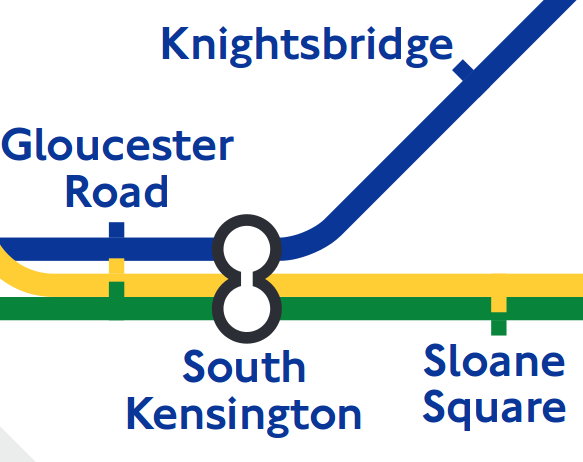
\includegraphics[scale=0.2]{tube_example.png}\\
Figure 13. Sample section of the Tube network.
\end{center}
The edge South Kensington (SK) to Knightsbridge (KB) has a cost of just $2.5$ as part of the route Gloucester Road--SK--KB, but has a cost of $10.17$ as part of the route Sloane Square--SK--KB due to needing to change trains at SK. We thus needed to keep track of which line and direction we were currently travelling on, to determine when to factor in the cost of changing trains. \\\\Furthermore, while we were unable to come up with any specific examples, we were aware of the possibility that suboptimally reaching a station via a different line and/or direction \textit{could} be part of an optimal route to another station. Consider that if from some station $A$ it took 30 minutes to arrive at SK by the westbound District, but 31 minutes to arrive at SK via the eastbound Piccadilly, following the route arriving at SK via the eastbound Piccadilly would still lead to reaching Knightsbridge more quickly ($31 + 2 < 30 + 10.17$). Hence, contrary to a typical best-first search we also needed to explore suboptimal paths to nodes where the time was within a tolerance margin of the best found time so far (\texttt{kMaxDetourEstimate}, set at 20 minutes). \\\\
The simulator would explore our internal model of the Tube network and then output a time matrix which expresses the time required to travel between any pair of stations in the Tube network. We have checked the reasonability of this model with the Transport for London Journey Planner; see section 5.1.2 for more detail on our testing strategies.
\subsection{Constructing \texttt{SimpleTravelTimeComputer}}
The \texttt{TubeNetwork} model only solves the problem of finding the time taken from one tube station to another; we needed a way to calculate the time taken to travel between a pair of arbitrary coordinates. While we have Tube support as described in section 4.4.3, it may not always be in our best interests to actually use the Tube even if available -- walking may be a faster option. Hence, \texttt{SimpleTravelTimeComputer} needs to support both walking and using the Tube (possibly including walking to Tube stations, of course). \\\\
As we are only supporting the city of London (in line with our customer's requirements), it seems reasonable to assume that one can always walk from the source to the destination. The straight-line distance between a pair of coordinates can be calculated by the \textit{haversine formula}. \cite{haversine} Clearly, it is not always possible to walk in a straight line from origin to destination; our implementation of \texttt{SimpleTravelTimeComputer} thus finds walking time by multiplying the straight-line distance by a factor of $1.25$ before dividing by the user's walking speed (which can be user-specified, though we typically use $5.0$ km/h). \\\\
In order to use the Tube, we would need to, from the origin, walk to a Tube station, use the Tube to travel to another station, and then walk from said other station to the destination. Importantly, it is not sufficient to simply choose the nearest station, seeing as different stations clearly have different lines going through them (for example, if one is in the Chinatown area of London and travelling to Paddington, while Leicester Square might be the nearest station it would probably be a better choice to walk to nearby Piccadilly Circus, for the Bakerloo Line). However, examining every possible combination of starting and ending stations is inefficient and seems unnecessary. 
\\\\We thus struck a compromise by considering the three nearest stations to the origin and three nearest to the destination; we would consider each of the 9 possible pairs of stations (one each near the origin and destination), and choose the pair yielding the best timing. This would be compared against the time for walking directly, and the overall best time would be returned.
\section{Travelling Salesman Problem}
Determining the most efficient route which users should take to complete their errands amounts to solving the asymmetric \textit{Travelling Salesman Problem}. This may be stated as finding the Hamiltonian cycle of minimum weight in an underlying graph \cite{tsp-def}, where locations are nodes and the routes between each pair of locations are edges. The weight of each edge is then the time required to travel from the starting to ending location. For our application, we have assumed that the underlying graph is 
\begin{itemize}
\item \textbf{directed}; this is necessary as edge weights may be (and often are) asymmetric.
\item \textbf{complete}; we are able to determine the time required to travel between any pair of coordinates.
\end{itemize}
The TSP is NP-hard \cite{tsp-np-hard} and thus we presently do not know of algorithms that solve it more quickly than in exponential time.
\subsection{Designing \texttt{TspSolver}}
\begin{center}
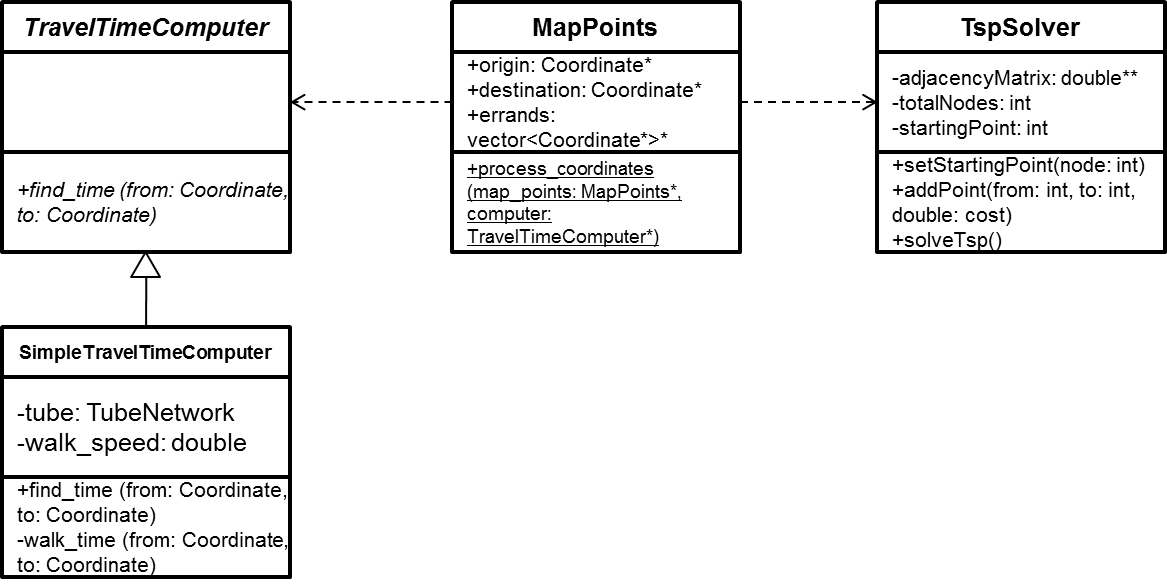
\includegraphics[scale=0.6]{uml_tsp.png}\\
Figure 14. UML Class Diagram of TSP-related classes.
\end{center}
Given an \texttt{origin} and several \texttt{waypoints}, the role of the \texttt{TspSolver} class is to find an optimal (or near-optimal) route, that begins and ends at the \texttt{origin} and visits all \texttt{waypoints} in some order. The class uses an adjacency matrix for internal representation of the data -- this is appropriate since fast ($O(1)$) lookup is required, and the graphs we are processing are complete graphs (so using $O(n^2)$ memory is unavoidable). \\\\
As we need to balance the requirements of having users receive a suitable route fairly quickly, and providing users with an efficient route, our implementation of \texttt{solveTsp()} selects a suitable algorithm given the size of the problem to be solved. Our current implementation uses the Held-Karp algorithm for $n \leq 18$ and the nearest-neighbour and 2-opt heuristics for $n > 18$.\\\\
The \texttt{MapPoints} class serves as an adapter for the \texttt{TravelTimeComputer} (see section 4.4.2) and \texttt{TspSolver} classes; it uses the \texttt{TravelTimeComputer} to determine the time required to travel between each of the points, populates the adjacency matrix in \texttt{TspSolver} and then solves the TSP, returning a vector of \texttt{Coordinate}s indicating the order in which the waypoints should be visited. We used the Strategy Pattern for the \texttt{TravelTimeComputer} to allow for easier future extension of the logic of how we compute edge weights \cite{strategy-pattern}.
\subsection{Recursive Backtracking}
Where the number of errands $n$ is small, a backtracking approach may be reasonable; essentially, this involves trying all possible routes, determining their cost, and selecting the route with the minimum cost. Since every possible route is examined, this is clearly guaranteed to yield the optimal solution. However, there are $n!$ many possible routes. Thus, while pruning can be performed (for example, not investigating routes where the cost of visiting a subset of the points has already exceeded the best solution found so far), it appears difficult to reduce the asymptotic time complexity of this approach below $O(n!)$.
\subsection{Dynamic Programming and the Held-Karp Algorithm}
The \textit{Held-Karp algorithm} is a solution to the TSP based on dynamic programming \cite{dp}, and solves the TSP with optimality in $O(n^2 2^n)$ \cite{heldkarp}. There is a space tradeoff in that $O(n 2^n)$ space is required, however. \\\\
Let $S$ be a subset of the locations to be visited $L$, and $l \in S$; let $C(S, l)$ denote the minimum cost of visiting all locations in $S$ ending at $l$. Clearly, if location $0$ is the origin and $a_{ij}$ is the cost of travelling from $i$ to $j$, we then have the recurrence
\begin{align*}
C(\lbrace l \rbrace, l) = & a_{0l} \\
C(S, l) = & \min_{m \in (S - l)} C(S - l, m) + a_{ml} & (|S| > 1)
\end{align*}
Clearly, the overall minimum cost is then given by $\min_{l \in L} C(L, l) + a_{l0}$. We maintain a table of values of $C$ indexed by $S$ and $l$, compute each of the $n2^n$ entries using the recurrence above in linear time -- hence the overall runtime is $O(n^2 2^n)$. \cite{heldkarp}
\subsection{Nearest-Neighbour Heuristic}
A popular approach when recursive backtracking proves intractable could be to use the \textit{nearest neighbour heuristic} -- that is, selecting the nearest unvisited waypoint at each step. This heuristic often performs within 25\% of the \textit{Held-Karp lower bound} \cite{nnh}, and clearly runs in $O(n^2)$ time. However, there exist cases where this heuristic can fail spectacularly. Consider the following graph (with symmetric edge weights):
\begin{center}
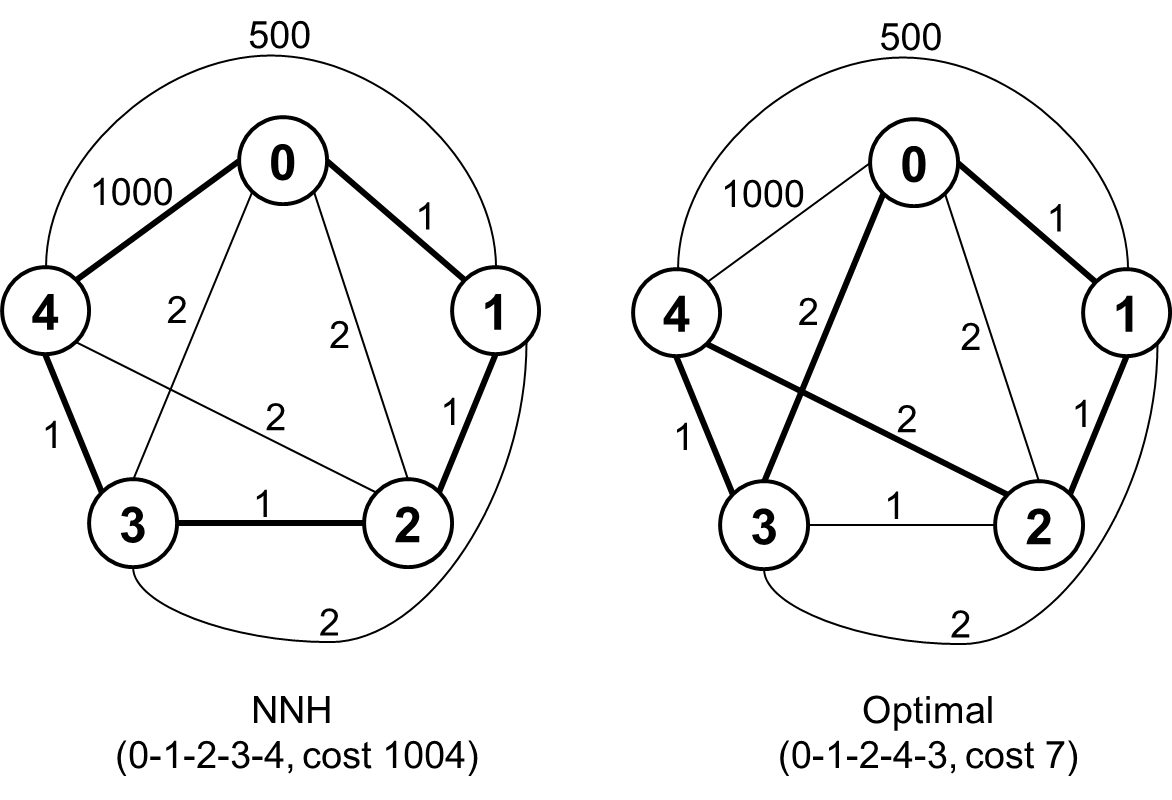
\includegraphics[scale=0.4]{nnh_fail.png}\\
Figure 15. Failing case for the nearest neighbour heuristic.
\end{center}
Relying on this heuristic alone can produce highly inefficient routes; we thus looked into ways to improve the routes returned.
\subsection{The 2-Opt Heuristic}
For larger problems, having generated a route (perhaps using the nearest neighbour heuristic), we can use local search heuristics to improve its efficiency. A \textit{2-opt move} involves removing two segments of our current route that don't share any nodes -- call these segments $(a, b)$ and $(c, d)$ -- and then rebuilding our route by adding back $(a, c)$, reversing the portion of our route that travelled from $b$ to $c$ (so this allows us to travel from $c$ to $b$), and adding $(b, d)$; we update our route if and only if this results in an improvement. We repeatedly check our route for 2-opt moves, stopping once no further improvement is possible. \cite{nnh,tsp-heuristics} Consider the following example:
\begin{center}
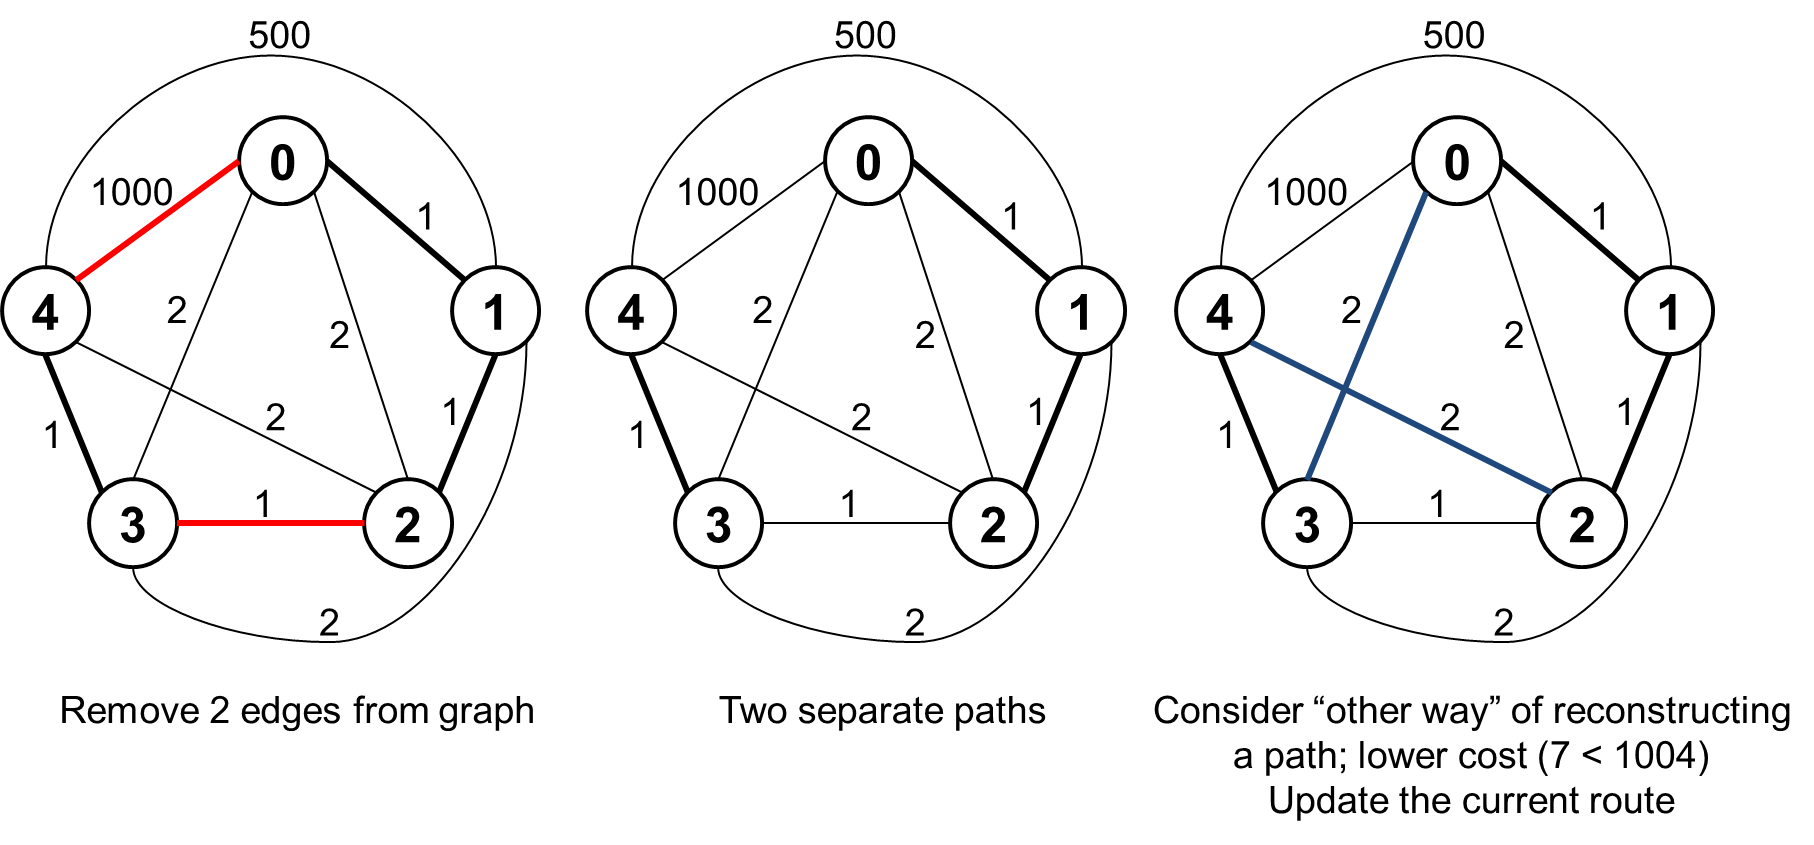
\includegraphics[scale=0.4]{2_opt.png}\\
Figure 16. 2-Opt transformation of the ``failed" NNH approach to the optimal solution.
\end{center}
2-Opt typically results in tours with costs less than 5\% above the Held-Karp lower bound, a significant improvement. \cite{nnh} The original algorithm for the symmetric TSP runs in $O(n^2)$; since we need to recompute the cost when reversing the route, however, for our asymmetric adaptation there is an additional cost of $O(n)$ when each pair of edges is considered -- hence, our implementation is $O(n^3)$. This is still certainly tractable for $n < 1000$, and we do not expect users to indicate this many errands. \\\\
Local search heuristics that explore a larger search space (for example, the general case of $k$-opt heuristics, which delete $k$ edges at a time and consider all possible ways to reconstruct a route, or the Lin-Kernighan algorithm which selects values of $k$ at each $k$-opt iteration step) are possible options as well, though they trade off speed and ease of implementation for the additional potential route quality. \cite{tsp-heuristics}
\subsection{Generalised Travelling Salesman Problem (GTSP)}
Our team also incorporated support for automatically selecting suitable locations for users given their errands. This is an instance of the \textit{Generalised} Travelling Salesman Problem (GTSP); nodes in our graph are partitioned into several subsets, and we need to find the lowest cost path visiting a node from each subset \cite{gtsp-transform}.
\\\\
We have implemented the \texttt{GtspSolver} class which is able to cope with the GTSP. The solver uses a variant of recursive backtracking as discussed in section 4.5.2 for smaller instances (where we have $k \leq 3$ clusters and $n \leq 40$ nodes total); it uses a genetic algorithm \cite{gtsp-ga} to approximate somewhat larger instances of the problem (where we have $k \leq 20$ clusters and $n \leq 300$ nodes total), as discussed in section 4.5.7, and finally uses a nearest-neighbour heuristic for even larger problems.
\subsection{A Genetic Algorithm for the GTSP}
The backtracking solution for the Generalised Travelling Salesman Problem (GTSP) was clearly not ideal for big cases. The use-case of our application poses quite a pathological example because of the way clusters are formed. When one searches for, for example, ``Grab a coffee", there are a lot of coffee shops which will come up (for a 500 meters radius in South Kensington at least 20), which means we can have at most 3 clusters before the backtracking algorithm begins to become intractable.
\\\\
The use of heuristics is not only a convenience, but a necessity in our application. We experimented with a couple of ideas and we decided that the Genetic Algorithm approach by John Silberholz and Bruce Golden is the best approach we can have to this problem \cite{gtsp-ga}. It also presented an interesting idea we decided to experiment with.
\\\\
A \textit{genetic algorithm} (GA) is a heuristic that mimics the process of natural selection. The strongest individuals mate, combine their genes and produce offspring which join the population, while the weakest individuals die, leaving the population. In our case, an individual is a solution to the GTSP problem; the strongest individuals are those solutions which have smaller (time) cost and reproduction is the process by which we combine two strong individuals, trying to create a new, possibly stronger one. We will call each reproduction state an iteration. After a certain number of iterations, the Genetic Algorithm converges towards a local minimum. The parameters of the algorithm we have implemented are presented below:
\subsubsection{Chromosome Representation}
We represent each chromosome as a path, as it is the most natural way to do so. For instance, the chromosome \texttt{( 1 4 2 )} represents a path that starts from node 1, goes to nodes 4, then 2, and finally returns to node 1.
\subsubsection{Population Initialization}
We are going to use 50 chromosomes as our population size. The initialization is done by randomly creating 50 valid chromosomes and adding them to the population. 
\subsubsection{Crossover}
The technique we used for crossover is called ordered crossover (OX). Two chromosomes are selected, and for each, two random cut points are chosen. The distance between the two cut points is the same for both parents. A child is produced by keeping the nodes between the cut points fixed and then adding, in turn and wrapping around, the nodes from the second parent whose clusters do not correspond to the selected nodes in the first parent, in order, from the second cut.\\\\
For example \texttt{(1 | 5 4 | 3 2) x (2 | 3 5 | 1 4) => (3 5 4 1 2)}; (here, each node is assumed to be of a different cluster.)
\subsubsection{Reproduction}
At each iteration, we select 30 chromosomes for crossover as described above. They will produce 30 offsprings, which will replace the weakest 30 chromosomes of the population.
\subsubsection{Mutation}
In order to facilitate diversity and to avoid the possibility of getting stuck in a local minima, each offspring chromosome has a 5\% probability of being selected for mutation. For the selected chromosomes, two random cut points are chosen on the chromosome and the nodes between those points are reversed; an example of a mutation would be \texttt{(1 | 2 3 4 | 5) -> (1 4 3 2 5)} (the bars represent the cut points).
\subsubsection{Terminating Condition}
The algorithm terminates if the population did not produce a better solution (best chromosome) for 150 iterations. We have seen that this value works well in practice as it keeps the runtime small and the solution fairly close to an accurate one. 
\subsubsection{Solution Optimisation}
Instead of keeping a single population of chromosomes, we decided to keep 7 populations. After each population converged (see the aforementioned section on the terminating condition), all the results are put together in a combined population of 350 and GA iterations are applied on this up till convergence. All the parameters are kept the same (mutation rate, reproduction set size).
\subsubsection{Analysis}
We have observed that this approach behaves well for $3-20$ clusters of approximately 15 nodes each; therefore it is the first preferred method after the backtracking solution (which is guaranteed to be optimal). All of the variables used as parameters have been either taken from the reference research paper or obtained through experimentation. However, for problems growing beyond this size the algorithm begins to be too slow and we thus switched to the Nearest Neighbour heuristic.

\chapter{Intermediate Feedback}
As discussed in chapter 3, we built our application in an agile fashion: we worked through short, time-boxed iterations, and between each iteration user requirements can be added, modified and re-prioritised. As such, the more feedback we were able to obtain, the more confident we could be in the direction in which we head. This feedback was obtained through automated system tests, as well as from our stakeholders.
\section{Automated Testing}
As introduced in section 3.3.3, we made heavy use of automated testing in the development process; developers were required to write unit tests before pushing new features (and these tests would also be peer-reviewed). This was instrumental to our efficiency in developing \textit{BusyRoute}, as this provided system feedback which helped us to ensure correctness, avoid regressions, and minimise the time and cost of debugging. Our automated test suites allowed us to gather correctness and regression feedback from the system on each build/deploy. This frequent running of our tests resulted in very small windows during which code can become broken, and thus sources of code breakage were more quickly identifiable.\\\\
Our front-end was primarily written in JavaScript while the back-end consists of both JavaScript and C++; in this section we will detail our testing strategies for our code in each programming language.
\subsection{JavaScript Testing}
To some extent, system tests played a role in determining whether our system is easy and convenient to use. We ensure that our front end is working properly using \textit{Mocha} \cite{mocha}, a JavaScript testing framework. We found that Mocha tests provide a fluent interface, reading like a specification for the object being tested. Furthermore, an advantage that Mocha has over main alternatives \textit{qUnit} \cite{qunit} and \textit{Jasmine} \cite{jasmine} is that Mocha more easily supports testing of asynchronous methods \cite{js-test-comp}, which feature heavily in our design.
\begin{center}
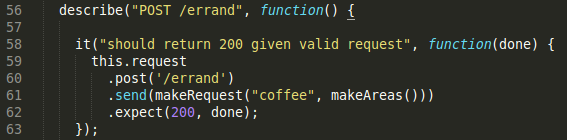
\includegraphics[scale=0.45]{mocha_test.png} \\
Figure 17. An example of a Mocha test.
\end{center}
We expected that busy users are likely to find slow systems inconvenient; and we implemented integration tests which monitor the performance (service time) of our system and fail should a significant performance regression arise. This was done by setting time limits with Mocha; a consideration to bear in mind, however, would be that such tests may be \textit{flaky}\footnote{such tests might fail non-deterministically} depending on the state of network connections and the availability of the Google Maps servers. \\\\
In terms of matching tasks to locations, we also evaluated our system's performance in this dimension by using system tests of our back-end that are driven by existing domain knowledge. For example, many team members personally know the area around South Kensington and Gloucester Road fairly well, and can identify that there are several places in these areas which individuals can go to complete certain tasks -- we checked that our algorithm to map these tasks to locations does recognise these places. 
\subsection{C++ Testing}
Much of our strategy for evaluating the correctness of the route planning portion of our back-end logic involves the use of automated tests to verify the accuracy and correctness of our code. This part of our back-end has been implemented in C++ and we are using the \textit{GoogleTest} framework \cite{googletest}, as it is flexible, simple to use and readily integrates with \textit{Jenkins} \cite{jenkins}, our continuous integration system. One of us also had substantial experience with this framework from his internship at Google last summer.
\\\\While much of the C++ code does not directly relate to usability, as discussed above we would not want the program to take excessive amounts of time when determining the best route -- we thus constrained the running time by introducing tests with timeouts, as shown in figure 18.
\begin{center}
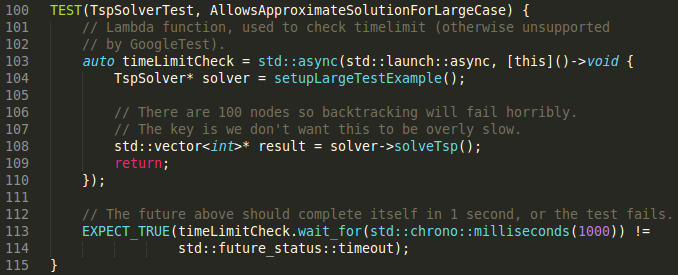
\includegraphics[scale=0.45]{google_test.png}\\
Figure 18. An example of a Google test for C++.
\end{center}
As discussed in chapter 4, we encountered two main algorithmic challenges involved in planning an optimal route -- determining the time taken to travel between potential points and then using this information to construct an optimal route.
\subsubsection{Modelling Edge Weights}
We developed an internal model for our application that found the time required to travel between two points, possibly using public transport. In order to verify the accuracy of our model of the London Underground network, we wrote unit tests that checked that the time taken between various locations would be within a certain margin of the times reported by the Transport for London \textit{Journey Planner} \cite{tfl-journey-planner} (for routes without disruptions). We observed that as the Journey Planner reported starting times for journeys, we would need to add approximately half the period of the available journeys to the time returned by the Journey Planner to come up with an estimate of the actual time a user might expect to need. \\\\
To check for correctness of how our application computed the time between two locations, we also wrote several unit tests involving a fake transport network that only had a few stations; for this simple network, we could easily manually compute the expected time required between various points and check our algorithm's output against it. This allowed us to ensure that said underlying components were behaving in line with expectations (regardless of the correctness of our Tube model).
\subsubsection{Constructing Optimal Routes}
Constructing an optimal route given the distances between locations involves solving the Travelling Salesman Problem (TSP), a graph problem involving finding the ``shortest" (or lowest-cost) path in a graph that visits each node once and returns to the origin. This is an NP-hard problem \cite{tsp-np-hard} and thus we presently do not know of algorithms that solve it more quickly than in exponential time. However, as maintaining a reasonable speed is important, we consider finding a route that is fairly close to the optimal solution acceptable.
\\\\ We have written unit tests for the back-end logic (for example, calculation of distance heuristics between points, functionality of data structures we have defined). We also constructed several simple cases for which we have manually determined the optimal solution, and check our algorithm's output against that. \\\\
Thankfully, as the TSP is a widely-studied problem, there are numerous TSP problems available online that are used as benchmarks for TSP solvers, such as that found in TSPLIB95 \cite{tsp-lib-95}. We compared the output of our algorithm with the optimal solutions (proven by various operations research techniques such as branch-and-bound); as long as our algorithm's output is within a tolerance margin (of say 25\%) from the best found solution, we consider it acceptable. Our algorithm is also not likely to have to deal with large numbers of locations ($n \geq 100$, for instance), so for efficiency of running said tests we have not considered very large instances of the problem.
\section{Intermediate Feedback from Stakeholders}
Our many aforementioned stakeholders provide us with many sources of such feedback, both in terms of how our product was evolving, as well as how we were working as a team. In this section we will explain how we gathered and used both types of feedback during our development process.
\subsection{Product Feedback}
\subsubsection{Gathering Feedback}
\begin{center}
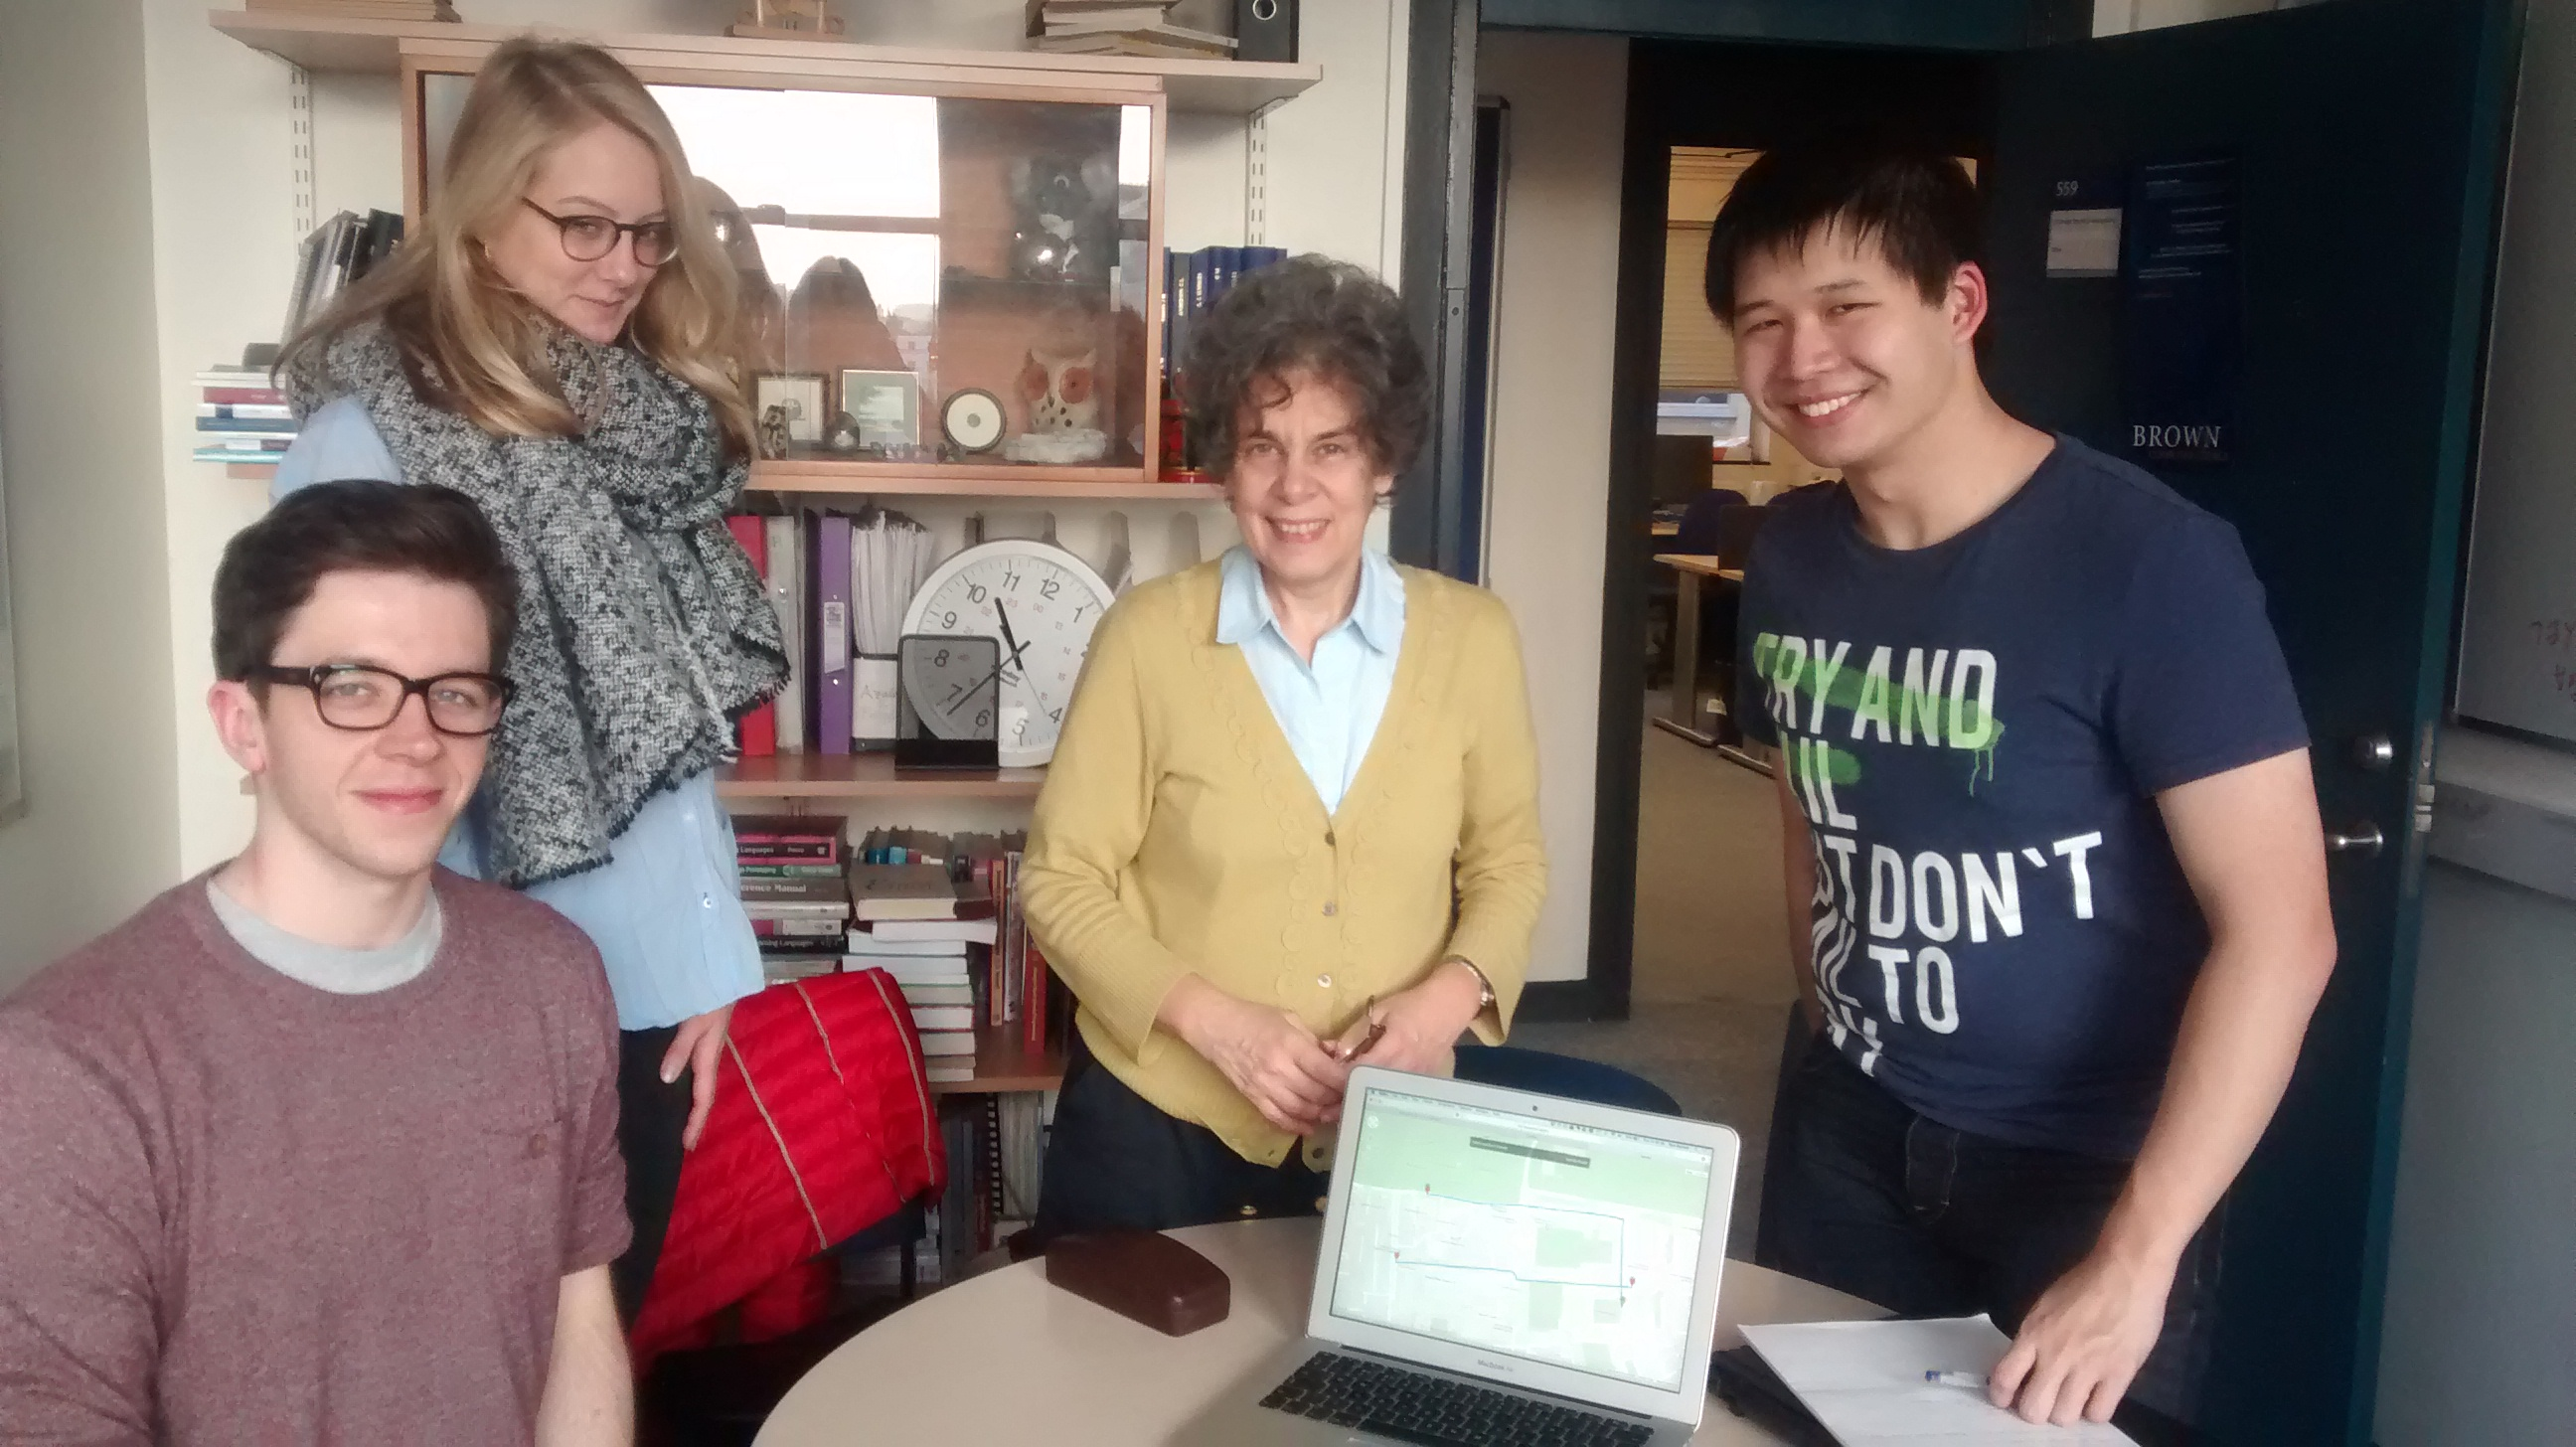
\includegraphics[scale=0.12]{sophia_1.png}\\
Figure 19. Sprint Demo meeting with our PS.
\end{center}
We hold different types of relationships with our various stakeholders, and so our methods of gathering feedback among them vary. With our PS, we held weekly Sprint Demo meetings, where we demonstrated the result of our work through the terminating iteration. During these meetings, the PS offered her opinion on what we have done, compared our work to her brief from the previous week's meeting, and outlined the direction in which she would like us to head during the next iteration. \\\\
We wanted a way to be able to demonstrate specific versions of our application to a wider group of critics. Using our development environments to demonstrate this proved to be somewhat difficult, and so we set up multiple so-called demo environments (see section 3.3.5 for more details). This provides us with a simple way for all team members to access the same specific version(s), without needing to affect his local workspace. \\\\
Using these environments, we have carried out hallway testing with other students (a key subset of our target user base of ``busy people"), as well as cross-validation among team members. We considered the possibility of carrying out A/B testing, using our multiple demo environments. However, since our sample size was somewhat limited (owing to time, manpower and budget constraints), we determined that it would be difficult to make statistically significant observations, and so did not carry out this form of testing. \\\\ 
In addition to demonstrating our work, we have also discussed various ideas concerning our product (such as possible features or user interface decisions) with our coursemates. We have incorporated some of this feedback into our project -- for example, we initially considered having the task input box overlaid on top of the map as opposed to in a separate panel to the left. Many students whom we interviewed did not like this, however, and preferred the input interface and map to be separate -- thus, we changed it accordingly.\\\\
Following our Sprint Demo each week, we carried out a Sprint Planning meeting, which typically lasted for about 2 hours. Officially, Scrum would require the PS and other customers to be present \cite{scrum-meetings}, however due to their busy schedules they were unable to be. Therefore, we gathered as much feedback as possible in the Demo meeting to take through to Planning, and we also emailed the PS with a detailed report of our Planning meeting outcome, for approval before development begins.\\\\
We wanted to be able to collect comparable feedback from a wide group of users (perhaps beyond those we could reach with hallway testing), in order to identify different and mutual requirements and preferences. Our PS suggested that one way of collecting such feedback would be to design a script which, along with an appropriately configured demo environment, team members could use to individually and remotely gather customer responses. Please refer to Appendix B for this survey.
\\\\
We were also unable to have regular meetings with our other stakeholders. To prevent this from being problematic, the PS suggested that we design a prototype in the form of a slide deck, which we could present to various customers. Our prototype is designed to show the entire length of a user story. Please refer to Appendix C to see this prototype.
\subsubsection{Using Feedback Received}
We didn't just gather feedback for feedback's sake -- we obsessively used it to improve our product and workflow. Firstly, we used our feedback to prioritise our features. As mentioned in section 3.4.1, we use \textit{Trello} \cite{trello} for managing the flow of tasks from their origin in the Product Backlog through to being Approved. It is the first of these columns -- the Product Backlog -- which is most directly influenced by our feedback. We kept this column strictly ordered, according to our customer's preferences. \\\\
Our application is complex and consists of many layers algorithmically. During an early Demo meeting, our PS voiced preference for us to implement the optimal routing functionality of our application, using a set of given points to visit, before implementing the translation of high-level user errands to places where such errands can be completed. As we generally select the highest priority item(s) from the Product Backlog to work on during an iteration, this helped drive our Sprint plans as well.
\\\\
Our feedback from our customers and PS in particular helped us to determine if we were building the right thing. Since our Sprints were just one week long, we were able to demonstrate a stable version of our product weekly, and gather specific and detailed feedback. This frequency helps us to reduce the amount of work potentially wasted, should we have implemented functionality not in line with the PS' expectations or requirements.
\subsection{Process Feedback}
%Andrea
From the beginning of the project, we were aware that we had very limited time that we could allocate to it, needing to balance this with coursework, preparation for examinations and the search for work placements. Consequently, we constantly analysed our work processes to understand how to manage our resources correctly, improve our development process and achieve higher quality results. This would allow us to make the best use of our development time. \\\\
We held weekly Sprint Retrospective meetings together with our PS, which played a crucial role in gathering feedback to help us improve our workflow. During these meetings, we analysed our previous Sprint and discuss processes that have worked well, as well as potential areas for improvement \cite{sprint-retro}. We evaluated our Trello board and discuss the tasks that have been completed (or not) as well as our estimation of the scope of said tasks. Moreover, we discussed within the group and with our PS about the challenges we encountered during the previous week and how we dealt (or failed to deal) with them. \\\\
We have also been provided some degree of external feedback, from the Software Engineering (Practice) coursework -- both from the comments written on our work, and from the face-to-face review sessions we have had with the course leaders. For example, our feedback from the second piece of coursework on development processes reminded us of the potential benefits of writing automated integration tests (which have since been added to our C++ code).\\\\
We have been able to identify several issues which have limited our velocity. At times, these issues are fairly unpredictable and somewhat inevitable -- such as placement interviews. However, we have also found on several occasions that there were obstacles in our development workflow; being able to identify, address and overcome these obstacles improved our efficiency.\\\\
For example, a problem we faced in the initial phases of our project involved working on the visual features of our application. We wanted to be able to modify parts of the application and allow the other members of the team to easily visualise the complete product at that stage without pushing to the master branch; in one of our sprint retrospectives, we realised that having the ability to give the other members a link to demo a particular feature would save us an incredible amount of time. This led to our solution of developing demo environments (see section 3.3.5); they became a critical part of our workflow for the front-end, allowing team members to easily have a visual overview of changes.

\chapter{Evaluation}
\section{Determining Evaluation Metrics}
In order to determine how successful \textit{BusyRoute} was in helping improve users' itinerary planning experience, we felt that we should first consider how users derive value from \textit{BusyRoute} -- what \textit{BusyRoute} could provide that existing routing products did not do (or did not do well).
\subsection{Identifying Stakeholders}
Our product aims to serve the needs of busy people -- people who need to complete a series of tasks in an efficient manner. These tasks include a wide variety of fairly common actions, such as posting a letter or getting a coffee, that people from all walks of life are likely to need or want at some point. Furthermore, we have found that it is fairly common for people to need to complete multiple tasks under time constraints; thus, the potential user base for our application is large and fairly diverse.\\\\
The idea for this product was mooted by our Project Supervisor (PS) Professor Sophia Drossoupoulou; she wanted to find efficient ways of running her errands, whether personal or professional, and fitting them into her busy life as a working professional (in this specific case, an academic). We met with our PS at least once a week, which allowed us to frequently discuss our work as well as the direction of our project with her.\\\\
A second group of users would be students; this may have been advantageous as we had ready access to ourselves as well as to other students in the Department of Computing, and we were thus be able to identify this user group's priorities and key requirements more easily.  From our personal experience, the need to run several errands in a limited time (e.g. during lunch breaks) is not uncommon. \\\\
Finally, a third group of users we targeted was tourists and frequent travellers. The notion of having a limited time is clearly relevant for these users, as they will generally only be in the location they're visiting for a short time and might want to use their vacation time as efficiently as possible. We do have several relatives and personal friends who would fall into this category of users; that said, we were especially careful to not let them know that we're demoing our own product lest this bias their feedback.
\subsection{Gathering Requirements}
In order to determine the PS's requirements as well as those of fellow working professionals, we held initial planning meetings with her to discuss the overall direction of the project and what she would look for in the final product. Minutes were taken during these meetings to ensure that her requests were suitably considered and followed. Initially, we had difficulty deciding between several interesting routing problems; we contacted the PS and engaged with her in remote discussion over email to help us come to a decision. We also held weekly meetings with the PS to ensure that new and changing requirements are recognised; using Agile methods and working with an iterative approach helped us remain flexible with regard to potential changes in requirements (which we have experienced over the course of this project). A concern that the PS raised was that our application would need to be convenient to use -- this is especially relevant for busy people who would otherwise not bother with a routing application. \\\\
We also held internal brainstorming sessions at the beginning of the project, during which we tried to identify problems we faced when addressing the errands we had to run. We drew on our personal experience as students with fairly busy schedules. In addition, we also discussed our ideas with several straight-talking friends and coursemates, who were able to provide valuable feedback and ideas for our application. \\\\
We did not \textit{initially} consider tourists to be one of our major user groups. However, we found from our personal experiences with travelling on holiday as well as discussions with relatives and personal friends who are frequent travellers that our application could be useful. In particular, as tourists often come from a wider range of backgrounds than working professionals and students (who tend to be relatively comfortable with technology), a common requirement that many of these users expressed was that our system needs to be not just convenient, but also simple to use.
\subsection{Value Proposition}
With these requirements in mind, we constructed a Value Proposition Canvas which helped us reflect on how \textit{BusyRoute} could help satisfy our users' requirements, and better understand how features we developed would be beneficial for our customers \cite{vpc}.
\begin{center}
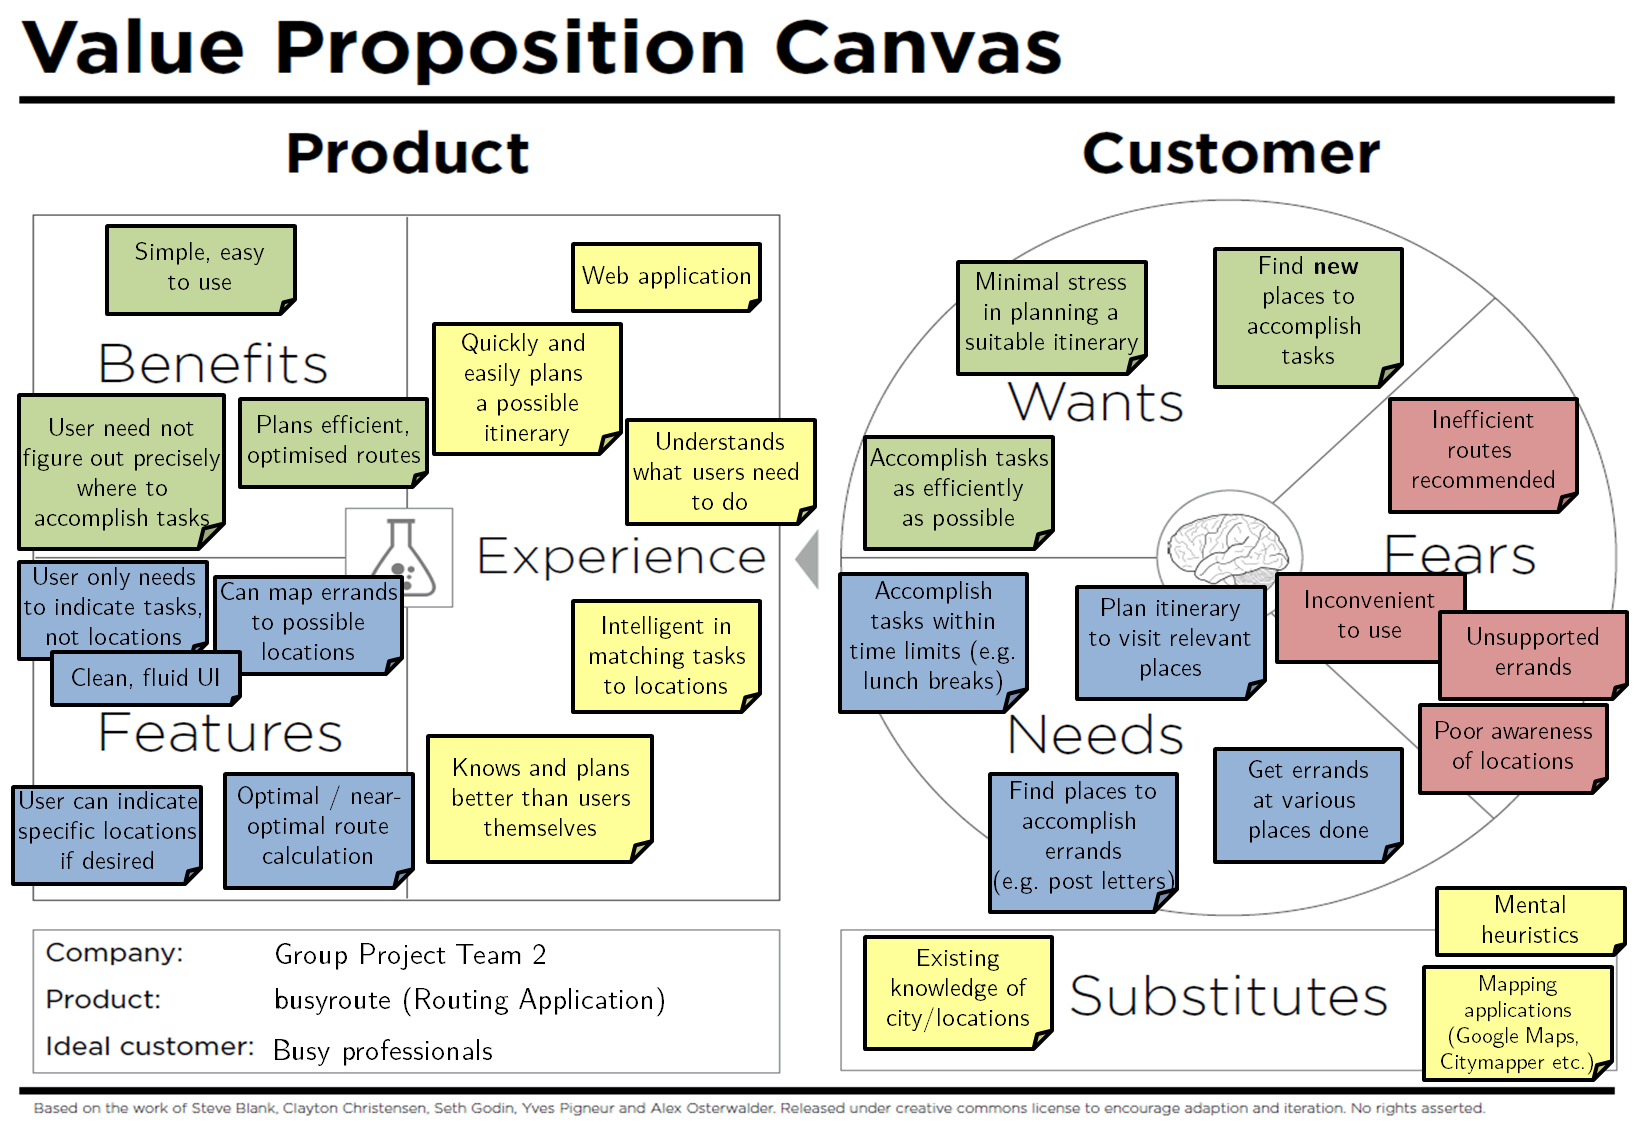
\includegraphics[scale=0.5]{vpc.png} \\
Figure 20. \textit{BusyRoute} Value Proposition Canvas.
\end{center}
In particular, there are three main benefits that \textit{BusyRoute} seeks to provide to customers:
\begin{enumerate}
\item Our application is simple and easy to use.
\item Our application works without the user needing to know precisely where tasks can be accomplished.
\item Our application helps users plan routes that are efficient and optimal or near-optimal.
\end{enumerate}
To some extent at least, we can measure the success of meeting customers' requirements by considering how successful \textit{BusyRoute} is in providing these benefits.

\section{Final Evaluation}
In this section, we will discuss various means by which we evaluated how far customers are likely to find \textit{BusyRoute} useful, considering the three main benefits it seeks to provide (as stated in section 6.1.3), and the results of said evaluation.
\subsection{Simplicity and Ease of Use}
This benefit was motivated by users' concerns that our routing application might be too difficult or inconvenient to use. As we have a sound knowledge of our application's user interface, it is difficult for us to fairly assess this on our own; thus, feedback from various users is essential for us to evaluate how far our application is simple, easy and convenient to use. \\\\
We met with our PS on a weekly basis, and used the demo environments mentioned in Section 3 to show her the front-end interfaces that we are providing to the user. During these meetings, a member of the team would take careful, detailed notes as to her reaction to our work, especially if we noticed that she has any difficulties in navigating the user interface. \\\\
In addition, we also performed hallway testing with users from the various stakeholder groups to help ascertain if our product was usable and/or if there seemed to be a customer interest in it. Typically, these tests involved asking users to carry out certain tasks on the application (for example, in the case of students, a possible scenario could be ``use the application to help you post a letter, visit a bank and print a document at the university".) We considered the time users take to complete these tasks (lower times are generally better), determined if they were able to understand the output presented, as well as noted if they struggled on any particular parts of the task. Eventually, we found that users did not have much difficulty using the application, mostly being able to plan a route within 3 minutes. Please consult Appendix B for details of our hallway tests. 
\begin{center}
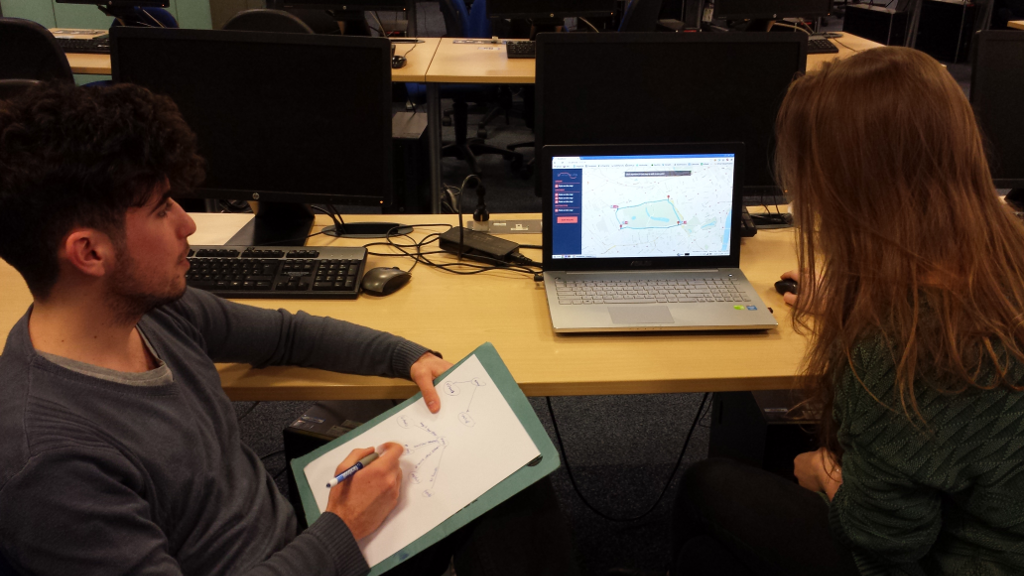
\includegraphics[scale=0.2]{hallway_1.png}
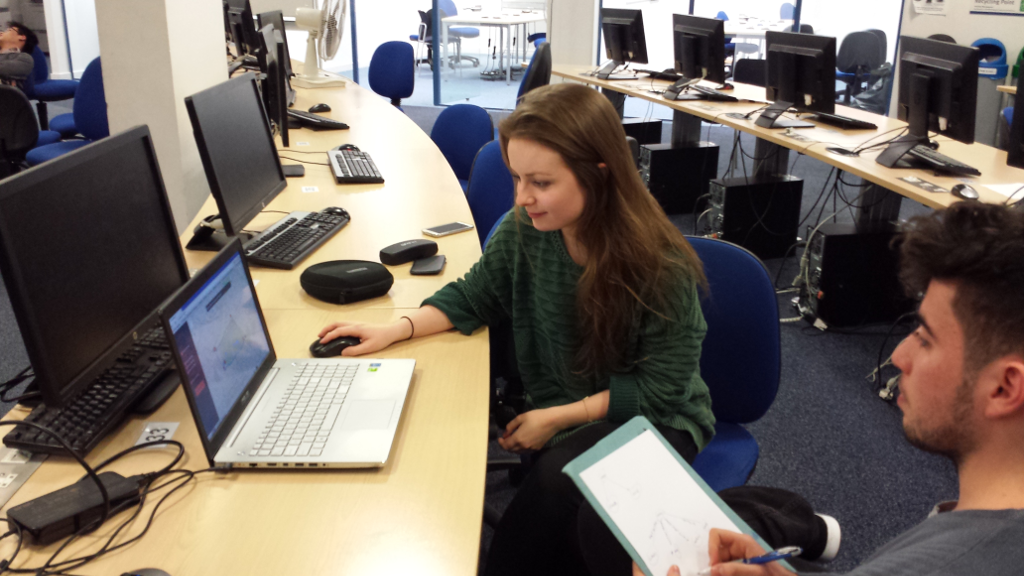
\includegraphics[scale=0.2]{hallway_2.png} \\
Figure 21. Hallway testing with a fellow student from DoC.
\end{center}
Hallway testing also highlighted just how important a feature intelligent place-selection is to users. No students specified any preference on where to withdraw cash, however obviously all chose Imperial's library for where to print his documents.\\
\\
A possible extension of this which would scale to a larger user-base could be to incorporate automated logging features into our front-end, so that timing data is automatically collected when users use the application (such as time taken for the user to add each task, find the map button, etc.) for later analysis.
\subsection{Determining Locations to Complete Tasks}
This benefit was motivated by users' desires to find new places to accomplish tasks, especially when this would mean that their errands could be completed more efficiently. It was also motivated by gaps in users' existing knowledge of locations where they can perform said tasks, which could have limited their ability to plan the most efficient routes.\\\\ 
To some extent, the quality of our results was verified by our system tests, which in turn relied on our external domain knowledge -- for example, team members were largely aware of the locations of banks around Imperial College, and our tests would verify that when running an errand to visit a bank, these locations would be considered. While said domain knowledge may not be perfect, having several different people in the team who could corroborate with one another helped. Furthermore, during the course of our hallway tests, we also asked users whether they notice any deficiencies/problems with regard to the locations identified; since errands were manually curated and places found using the Google Places API, most users seemed fairly satisfied with the locations identified by our application. \\\\
We acknowledge that it is not possible for our system to capture every possible task that a user might want to do; support for new errands often needs to be manually added. In order to alleviate this, we allow users to indicate specific points (where they know they can do what they need to) to include in the route. A possible extension could also involve developing a feedback or poll system which allows users to suggest possible future tasks that we should add support for.

\subsection{Planning Optimal / Efficient Routes}
This benefit was motivated by users' needs to plan itineraries to allow them to complete tasks within time limits, as well as their desires to accomplish said tasks as efficiently as possible.\\\\
As explained in section 5.1.2, system tests are instrumental in verifying the accuracy and correctness of our route planner. We developed an internal model for the London tube network, and performed cross-validation with the official Transport for London Journey Planner; we also tested several relevant classes on a fake transport network on which we manually determined the expected behaviour.
Furthermore, we wrote several integration tests involving possible real-life examples, that ensured that components were interfacing correctly. Our development process, by design, involves automatically pushing to a pre-production environment if all tests pass, waiting for manual approval before deployment to production (see section 3.3.7); we would typically also run manual acceptance tests in this pre-production environment as an additional precaution.
\begin{center}
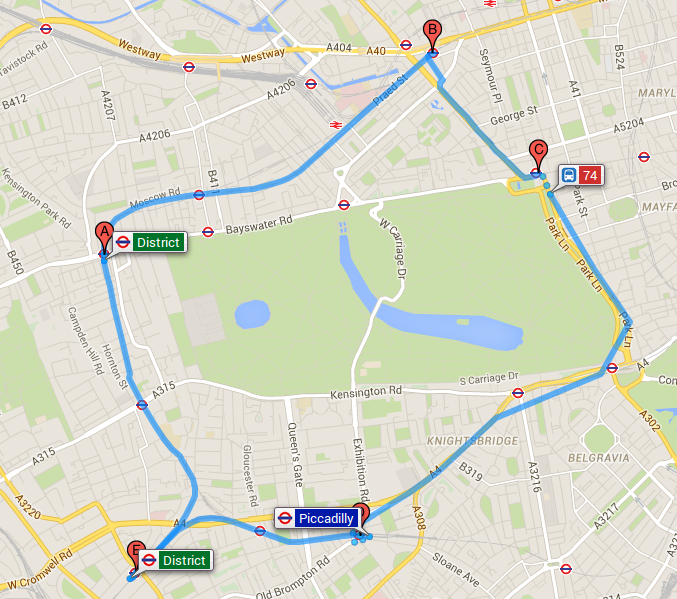
\includegraphics[scale=0.3]{eval_notubemodel.png}
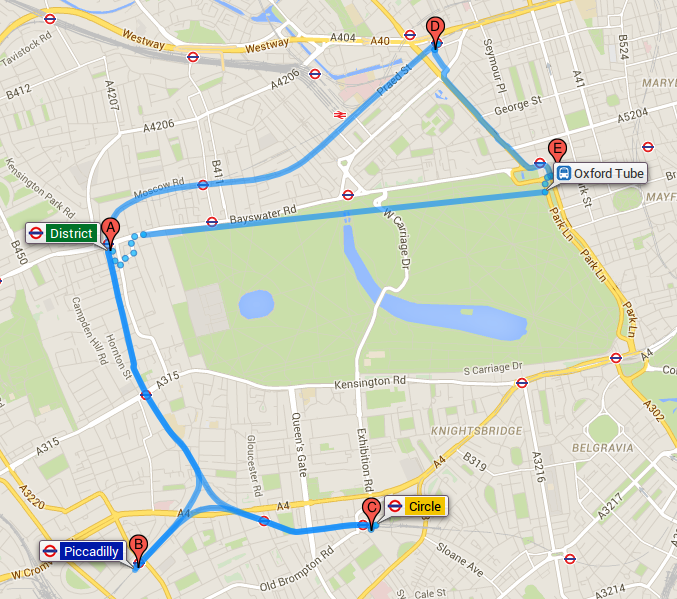
\includegraphics[scale=0.3]{eval_tubemodel_works.png} \\
Figure 22. Acceptance test verifying reasonability of the Tube model. The route on the left is planned without the Tube model; the route on the right is planned using the Tube model and is more efficient by 11 minutes, according to the TfL Journey Planner.
\end{center}
As a `sanity check' for the system, we also asked users for their opinions about the routes our algorithm selects during hallway tests, seeing if they can construct a better route. Studies have found that human performance on the TSP is fairly good, at least when the distance metric is Euclidean \cite{human-tsp}; this could perhaps provide a lower bound on the performance we require of our algorithm, as one of \textit{BusyRoute}'s intended user experiences is that the user finds that the application plans better than he can on his own\footnote{(Note that in practice, travel time between locations is actually \textit{not} Euclidean due to varying availability of different modes of transport from one location to another.)}. \\\\
Our application generally performed well in the hallway tests; users were satisfied with the routes provided and were not able to come up with a clearly better route on their own. However, we do acknowledge that our application does have limitations under certain cases that did not frequently arise in the hallway tests.
\\\\
\textit{BusyRoute} currently only considers two modes of transport when determining the order to visit locations: walking and using London Underground. Our sample of interviewees for the hallway testing were students at Imperial College London and thus likely to be based in central London, where tube coverage is much higher than in other parts of the city. Furthermore, we also observed that users frequently want to complete their errands fairly close to one another; for these cases, the fact that the only means of public transport we currently support is the Tube is not particularly critical (since the overhead involved in waiting for buses often makes walking or using the Tube a viable option as well).
\subsection{Overall Evaluation}
We feel that on the whole, \textit{BusyRoute} does provide value to its users, guiding them through a relatively seamless planning experience. The user interface presented is simple, functional and familiar, helping users construct plans with ease; this is backed up by a solid back-end which is able to both figure out where users might run their errands as well as how to efficiently accomplish these tasks, minimising time spent travelling. As a group, we are relatively satisfied with our final product.
\chapter{Conclusion}
\section{Reflections on Project Management}
As far as Agile methods were concerned, we found using one-week Sprint cycles fairly demanding on our schedule. Working with strict timeboxed iterations (as compared to projects in previous years) helped us evaluate our pace of work and ensure that we did not fall too far behind\footnote{Unfortunately, Hofstadter's Law \cite{hofstadter} still prevailed.}. Having regular weekly meetings with our PS also allowed us to regularly seek her advice and guidance on how to prioritise our product's features.
\\\\
We had weekly Sprint planning meetings; however, the changing commitments of team members each week occasionally resulted in not all members being in attendance at each meeting, and this proved disruptive to our workflow. This was somewhat inevitable given that we formed our team based on being comfortable working with one another; we are aware of groups that formed based on their module combination (and thus had minimal conflict in terms of lectures as well as coursework deadlines).
\\\\
Through the Software Engineering (Practice) course, we learned about potential issues with system setup and deployment of software to production; we used \textit{Vagrant} and \textit{Ansible} to standardise our local development environments with our production environment as discussed in section 3.3.2. This allowed us to verify that code working on our local machines would also run in production; we thankfully did not encounter `nasty surprises' when pushing code to our production environment.
\\\\
We were largely new to continuous integration practices. While we spent a fairly large amount of time configuring \textit{Jenkins}, our CI server, we found that it worked well, automatically deploying pushed code to our pre-production environment if it passed our tests. Pushing code frequently and keeping our master branch up to date was effective -- we were immediately informed when builds or tests failed, and code breakages could thus generally be isolated and fixed relatively quickly. We feel that the time spent in setting up \textit{Jenkins} was well-invested, considering the potential hours of debugging and/or merge conflicts that may have been averted by doing this.
\\\\
Throughout the project, we had a strong desire to write clean, correct code. We considered the possibility of using pair programming, but eventually rejected it as our individual schedules did not allow for this, using code reviews instead. In hindsight, we should have at least tried to use pair programming where possible, as we found that while reviews did mean that another developer had looked at and approved the code, interaction typically occurred only after much of the code had already been written. In pair programming, the ``driver" typically gives \textit{running commentary} on his code, and the ``navigator" can easily intervene, suggesting (possibly better) alternative solutions/implementations that the driver may not have thought of. \cite{pair-prog}
\\\\
The code review system did increase our Bus Factor as intended, however we're not entirely certain it was the best approach. During the middle of the Autumn Term when group members had many other responsibilities to deal with, it often introduced a significant time lag in our workflow, as code reviews (CRs) would often wait for a few days before getting completed. A possible solution to mitigate this could be to implement a time limit for performing CRs once assigned. 
\\\\
In addition, we found that team members tended to gravitate towards doing CRs on sections of the project or technologies that they knew best; this is reasonable as far as efficiency and review quality was concerned, but often led to just two developers rather than the whole team knowing about certain features. We could have used a tool that randomly assigned group members to CRs (rather than developers choosing which CRs they would perform); however, this does run the risk of slowing down the review process (if the selected developer happens to be particularly busy at that time, for instance).
\\\\
We also found that front-end changes often proved difficult to review; visual changes were often difficult to check with automated tests. As a result, we introduced demo environments as discussed in section 3.3.5. While we did initially spend quite a lot of time setting these environments up, we found that they did save us a lot of time later in the project when multiple developers simultaneously worked on different front-end features. They also had a side effect of allowing us to demonstrate different versions of our product.
\\\\
Compared to projects in previous years, our team was fairly large. We found that ensuring clear communication between team members was important to ensure work was not duplicated and deadlines could be met. We found Trello effective for keeping one another updated about the state of the project -- a team member who had found it unhelpful during the WebApp projects (team of 3) last year commented that he found it useful this time round. The Facebook group was also fairly effective in eliciting quick responses from teammates.
\section{Reflections on Product Design and Implementation}
During the development of our application, we had many choices to make in terms of programming languages and patterns. Having the flexibility to implement any part of our application in any language of our choice, and being able to choose any design patterns, forced us to reflect on the advantages of each approach, giving us a deeper understanding.
\\\\
We used two different languages for our server code: JavaScript and C++. We have not only learnt how to bridge interactions smoothly between components written in the two languages, but we also have learnt how to divide wisely the work between the two, trying to find the Pareto optimality between the efficiency of C++ and the flexibility of JavaScript.
\\\\
We used \textit{ExpressJS} for our server-side framework. Express is a minimal framework that does not enforce any particular design patterns. However, we realised that the MVC pattern works very well for our application. Thus, we learned how to structure our application using a framework that differently from bigger frameworks like Django and Rails does not implement the MVC pattern out-of-the-box.
\\\\
JavaScript is a peculiar language; despite the similarities with other languages, it is fairly different under the hood and it’s patterns differ greatly from what we are used to. During our project, we studied many JavaScript patterns to further the development of our application. Out of the many, the module pattern, consisting of wrapping the code in anonymous functions in order to not pollute the scope \cite{module-pattern}, together with \textit{Browserify}, helped to produce code that is clean and easy to understand (as we analysed in section 4.2.2).
\\\\
The TSP solver is a crucial component of our application. We spent a fair amount of time discussing its implementation. However, rather than implementing the algorithm from scratch we could have used an external library. Using such a library (like \textit{Concorde} \cite{concorde}, we would have saved time that could have been dedicated to other parts of the project; many libraries also implement more sophisticated heuristics that might approximate the TSP more accurately. On the other hand, using an external library would have been less flexible. \\\\
As discussed in section 4.2.2, we decided to not use a framework for the client-side. It is true that our product is a one-page application and many client-side frameworks such as \textit{AngularJS} and \textit{EmberJS} are not suited for our structure. However, using a smaller framework such as \textit{React} \cite{react}, we would have been able to render the Views on the client and this would have been beneficial for our application. In fact, by not rendering all the Views in the server we would have limited our use of \textit{jQuery} in our client-code and consequently our client code count have been kept cleaner.

\subsection{Third Party Services}
\textit{BusyRoute} relies heavily on \textit{Google Directions} and \textit{Google Places} APIs. Both services are free to use for making up to a maximum of 2500 and 1000 daily requests respectively. For BusyRoute in its current state, this poses no problem:
\begin{itemize}
	\item \textit{Google Directions }is called for finding a route between each pair of adjacent points on a user’s errand run. Based on our research, users on average use \textit{BusyRoute }when having 6 errands to complete. Resulting in 7 \textit{Google Directions }calls, the imposed request limit allows for $\sim$350 uses of \textit{BusyRoute }per day.
	\item \textit{Google Places }is called for identifying locations where a user can complete errands. As explained, when a user searches for places to carry out his $n^{\text{th}}$ errand, $n$ requests are made, searching near all of the previously-selected points. Based on an average of 6 errands, this results in 21 \textit{Google Places }calls, allowing for $\sim$50 uses of \textit{BusyRoute }per day.
\end{itemize}
It is clear that, should \textit{BusyRoute }take off, we could consider paying for additional usage, and/or researching additional APIs that may offer similar functionality.

\section{Possible Extensions}
Throughout the project, we have carefully considered our design decisions, aiming as far as possible to ensure that our code was open to extension. 
Our group considered several possible additional features we could add to \textit{BusyRoute} that we would like to have worked on had we more time:
\begin{itemize}
\item \textbf{Considering Additional Travel Options} -- Currently, \textit{BusyRoute} only considers the possibilities of walking and taking the Tube when deciding on the best order to visit locations. As discussed in section 4.4.2, adding additional public transport networks such as the DLR or Bus would entail writing a new concrete implementation of \texttt{TransportNetwork} and \texttt{TravelTimeComputer}. 
\item \textbf{Additional Location Support} -- \textit{BusyRoute} currently only supports routes within London; while the Google Places API that we use for location finding is international, the logic for planning routes using public transport is currently limited only to London Underground. Adding support for other public transport systems (such as the MTR system in Hong Kong, for example) could be implemented in the same way as adding additional travel options.
\item \textbf{Precedence Constraint Support} -- In our hallway tests, several users highlighted use-cases where the order in which one completes one's errands mattered -- for example, one might wish to withdraw money \textit{before} going shopping or getting coffee. Currently, \textit{BusyRoute} does not support precedence constraints -- however, approaches based on genetic algorithms have been used to approximately solve the TSP with such constraints \cite{ga-tsp}; hence this does appear feasible.
\item \textbf{Improved TSP Approximation} -- As discussed in section 4.5, we employed recursive backtracking where the number of errands $n \leq 8$; when $n > 8$ we currently use the Nearest Neighbour and 2-Opt heuristics. There exist more sophisticated approaches such as the 3-Opt heuristic or Lin-Kernighan algorithm \cite{tsp-heuristics}, which may achieve better approximations.
\item \textbf{Future Planning Support} -- Currently, our application assumes that users are beginning their route at the same time the application is used; we could add an option to allow users to indicate that they wish to start their journey at a later time -- this is necessary since it may affect the availability of public transport routes.
\end{itemize}


\begin{appendices}
%BIBLIOGRAPHY
\begin{thebibliography}{99}
% BIBLIOGRAPHY FOR SECTION 1
\bibitem{yplan} ``YPlan", \texttt{https://yplanapp.com} [accessed $\text{2015-01-12}$]
\bibitem{coffee-in-touch} ``Coffee(In)Touch", \texttt{http://www.coffeeintouch.com} [accessed $\text{2015-01-12}$]
\bibitem{google-maps} ``Google Maps", \texttt{http://google.co.uk/maps} [accessed $\text{2015-01-09}$]
\bibitem{citymapper} ``Citymapper", \texttt{http://citymapper.com} [accessed $\text{2015-01-09}$]
% BIBLIOGRAPHY FOR SECTION 2
\bibitem{tfl-journey-planner} ``Journey Planner", \texttt{http://www.tfl.gov.uk/plan-a-journey/} [accessed $\text{2015-01-09}$]
\bibitem{gmaps-no-dir}
``Google Maps JavaScript API v3",\\
\texttt{http://developers.google.com/maps/documentation/javascript/directions}
[accessed $\text{2015-01-07}$]

% BIBLIOGRAPHY FOR SECTION 3
\bibitem{sprint-len}
Roock, Stefan. ``Shades of Scrum: Sprint length",\\ \texttt{https://stefanroock.wordpress.com/2012/12/20/shades-of-scrum-Sprint-length/} [accessed $\text{2014-12-29}$]
\bibitem{sprint-small-gd}
Levison, Mark. ``Choosing a Sprint Length - Shorter Trumps Longer",\\
\texttt{http://agilepainrelief.com/notesfromatooluser/2013/07/choosing-Sprint-length-\\shorter-trumps-longer.html} [accessed $\text{2014-12-29}$]
\bibitem{sprint-backlog} ``Scrum Product Backlog and Agile Product Backlog Prioritization",\\
\texttt{http://www.mountaingoatsoftware.com/agile/scrum/product-backlog} [accessed $\text{2014-12-29}$]
\bibitem{sprint-middle} Rawsthorne, Dan, and Shimp, Doug. ``Scrum in a Nutshell",\\
\texttt{https://www.scrumalliance.org/community/articles/2009/december/scrum-in-a-nutshell} [accessed $\text{2014-12-29}$]
\bibitem{scrum-master}
``The ScrumMaster",\\
\texttt{http://www.mountaingoatsoftware.com/agile/scrum/scrummaster}
[accessed $\text{2014-12-29}$]
\bibitem{xp-scrum-diff}
Cohn, Mike. ``Differences between Scrum and Extreme Programming",\\
\texttt{http://www.mountaingoatsoftware.com/blog/differences-between-scrum-and-extreme-\\programming} [accessed $\text{2014-12-29}$]

\bibitem{git}
``Git", \texttt{http://git-scm.com/} [accessed $\text{2015-01-09}$]
\bibitem{github}
``GitHub", \texttt{http://github.com/} [accessed $\text{2015-01-09}$]
\bibitem{jenkins}
``Welcome to Jenkins CI!", \texttt{http://jenkins-ci.org} [accessed $\text{2015-01-09}$]
\bibitem{vagrant}
``About Vagrant -- Vagrant.", \texttt{http://www.vagrantup.com/about.html} [accessed $\text{2015-01-09}$]
\bibitem{ansible}
``Ansible is Simple IT Automation", \texttt{http://www.ansible.com/home} [accessed $\text{2015-01-09}$]
\bibitem{puppet}
``Puppet Labs: IT Automation Software for System Administrators", \texttt{http://puppetlabs.com/} [accessed $\text{2015-01-09}$]
\bibitem{chef}
``Chef - Code Can", \texttt{http://chef.io/} [accessed $\text{2015-01-09}$]

\bibitem{tdd}
Williams, Laurie, E. Michael Maximilien, and Mladen Vouk. ``Test-driven development as a defect-reduction practice." \textit{Software Reliability Engineering, 2003. ISSRE 2003. 14th International Symposium on.} IEEE, 2003.
\bibitem{googletest}
``googletest -- Google C++ Testing Framework", \texttt{http://code.google.com/p/googletest/} [accessed $\text{2015-01-09}$]
\bibitem{mocha}
``Mocha -- the fun, simple, flexible JavaScript test framework",
\texttt{http://mochajs.org/} [accessed $\text{2015-01-09}$]
\bibitem{pair-program}
Williams, Laurie, et al. ``Strengthening the case for pair programming." \textit{IEEE software} 17.4 (2000): 19-25.
\bibitem{github-pull-req}
``Using pull requests - User Documentation", \\
\texttt{http://help.github.com/articles/using-pull-requests/} [accessed $\text{2015-01-07}$]
\bibitem{ci}
Fowler, Martin, and Foemmel, Matthew. ``Continuous integration." (Thought-Works) \texttt{http://www.thoughtworks.com/Continuous Integration.pdf} [accessed $\text{2014-12-29}$]
\bibitem{jenkins-github-plugin}
``GitHub Plugin -- Jenkins Wiki",
\texttt{https://wiki.jenkins-ci.org/display/JENKINS/GitHub+Plugin}
[accessed $\text{2015-01-09}$]
\bibitem{trello}
``Trello", \texttt{http://trello.com} [accessed $\text{2015-01-09}$]
\bibitem{jira}
``JIRA Agile $|$ Atlassian", 
\texttt{https://www.atlassian.com/software/jira/agile} [accessed $\text{2015-01-09}$]

% BIBLIOGRAPHY FOR SECTION 4
\bibitem{google-directions}
``The Google Directions API - Google Developers", \\ \texttt{https://developers.google.com/maps/documentation/directions/} [accessed $\text{2015-01-11}$]
\bibitem{separate-concerns}
Hursch, Walter L., and Cristina Videira Lopes. ``Separation of concerns." (1995).
\bibitem{separate-concerns-2}
Sullivan, Kevin J., et al. ``The structure and value of modularity in software design." \textit{ACM SIGSOFT Software Engineering Notes} 26.5 (2001): 99-108.

\bibitem{laravel}
``Laravel -- The PHP framework for web artisans.", 
\texttt{http://laravel.com/} [accessed $\text{2015-01-11}$]
\bibitem{rails}
``Ruby on Rails", \texttt{http://rubyonrails.org} [accessed $\text{2015-01-11}$]
\bibitem{django} ``The Web framework for perfectionists with deadlines $|$ Django", \texttt{http://www.djangoproject.com} [accessed $\text{2015-01-11}$]
\bibitem{expressjs}
``Express -- Node.js web application framework", \texttt{http://expressjs.com/} [accessed $\text{2015-01-11}$]
\bibitem{nodejs-popular}
``Usage Statistics and Market Share of Node.js for Websites, January 2015", \texttt{http://w3techs.com/technologies/details/ws-nodejs/all/all} [accessed $\text{2015-01-11}$]
\bibitem{handlebars}
``Handlebars.js: Minimal Templating on Steroids", \texttt{http://handlebarsjs.com/} [accessed $\text{2015-01-11}$]
\bibitem{js-frameworks}
``The 10 hottest JavaScript framework projects $|$ InfoWorld",\\ \texttt{http://www.infoworld.com/article/2612250/application-development/the-10-hottest-\\javascript-framework-projects.html} [accessed $\text{2015-01-11}$]
\bibitem{browserify}
``Browserify", \texttt{http://browserify.org/} [accessed $\text{2015-01-11}$]
\bibitem{module-pattern}
``JavaScript Module Pattern: In-Depth", \texttt{http://www.adequatelygood.com/JavaScript-Module-\\Pattern-In-Depth.html} [accessed $\text{2015-01-11}$]
\bibitem{grunt}
``Grunt: The JavaScript Task Runner",
\texttt{http://gruntjs.com/} [accessed $\text{2015-01-11}$]
\bibitem{sass}
``Sass: Sass Basics", \texttt{http://sass-lang.com/guide} [accessed $\text{2015-01-11}$]
\bibitem{jade}
``Jade -- Template Engine", \texttt{http://jade-lang.com/} [accessed $\text{2015-01-11}$]
\bibitem{jquery-autocomplete}
``Autocomplete $|$ jQuery UI", \texttt{http://jqueryui.com/autocomplete/} [accessed $\text{2015-01-11}$]
\bibitem{fuse-js}
``Fuse.js $|$ K.Risk -- JavaScript Refined", \texttt{http://kiro.me/projects/fuse.html} [accessed $\text{2015-01-11}$]
\bibitem{gmaps-js}
``Google Maps JavaScript API v3 -- Google Developers",\\ \texttt{https://developers.google.com/maps/documentation/javascript/}
[accessed $\text{2015-01-11}$]
\bibitem{openstreetmap}
``OpenStreetMap", \texttt{http://www.openstreetmap.org} [accessed $\text{2015-01-11}$]
\bibitem{i18n}
``AgileConnection $|$ Internationalization Best Practices for Agile Teams", \texttt{http://www.agileconnection.com/article/internationalization-best-practices-agile-\\teams} [accessed $\text{2015-01-11}$]

\bibitem{google-places}
``Google Places API -- Google Developers", \texttt{https://developers.google.com/places/} [accessed $\text{2015-01-11}$]
\bibitem{google-places-types}
``Supported Place Types - Google Places API -- Google Developers", \texttt{https://developers.google.com/places/documentation/supported\_types} [accessed $\text{2015-01-11}$]


\bibitem{tube-stat}
``London Key Facts and Statistics - London Councils"\\
\texttt{http://www.londoncouncils.gov.uk/londonfacts/default.htm?category=12} [accessed $\text{2015-01-08}$]
\bibitem{foi-chris}
``Gate-to-platform and interchange walking times"\\
\texttt{https://www.whatdotheyknow.com/request/gate\_to\_platform\_and\_interchange}
[accessed $\text{2015-01-08}$]
\bibitem{tfl-wtts}
``Working Timetables (WTT)"\\
\texttt{https://www.tfl.gov.uk/corporate/publications-and-reports/working-timetables} [accessed $\text{2015-01-08}$]
\bibitem{haversine}
Veness, Chris. ``Calculate distance and bearing between two Latitude/Longitude points using Haversine formula in JavaScript." (2011)

\bibitem{tsp-def}
Wallis, Walter D. \textit{A beginner's guide to graph theory.} Boston: Birkhauser, 2000.
\bibitem{tsp-np-hard}
Lenstra, Jan Karel, and A. H. G. Kan. "Complexity of vehicle routing and scheduling problems." \textit{Networks} 11.2 (1981): 221-227.
\bibitem{strategy-pattern}
``Strategy Design Pattern", \texttt{http://sourcemaking.com/design\_patterns/strategy} [accessed $\text{2015-01-10}$]
\bibitem{dp}
``Algorithm Tutorials",
\texttt{http://www.topcoder.com/tc?d1=tutorials\&d2=dynProg\&module=Static}
[accessed $\text{2015-01-10}$]
\bibitem{heldkarp}
Held, Michael, and Richard M. Karp. "A dynamic programming approach to sequencing problems." \textit{Journal of the Society for Industrial \& Applied Mathematics} 10.1 (1962): 196-210.
\bibitem{nnh}
D.S. Johnson and L.A. McGeoch, ``The Traveling
Salesman Problem: A Case Study in Local Optimization",
November 20, 1995.
\bibitem{tsp-heuristics}
Rosenkrantz, Daniel J., Richard E. Stearns, and Philip M. Lewis, II. "An analysis of several heuristics for the traveling salesman problem." \textit{SIAM journal on computing} 6.3 (1977): 563-581.

\bibitem{gtsp-transform}Behzad, Arash, and Mohammad Modarres. ``A new efficient transformation of the generalized traveling salesman problem into traveling salesman problem." \textit{Proceedings of the 15th International Conference of Systems Engineering}. 2002.
\bibitem{gtsp-ga}
Silberholz, John, and Bruce Golden. "The generalized traveling salesman problem: A new genetic algorithm approach." \textit{Extending the horizons: advances in computing, optimization, and decision technologies.} Springer US, 2007. 165-181.

% BIBLIOGRAPHY FOR SECTION 5
\bibitem{qunit}
``QUnit", \texttt{http://qunitjs.com/} [accessed $\text{2015-01-08}$]
\bibitem{jasmine}
``Jasmine: Behavior-Driven JavaScript", \texttt{http://jasmine.github.io/} [accessed $\text{2015-01-08}$]
\bibitem{js-test-comp}
Groat, Kevin. ``Which JavaScript Test Library Should You Use? QUnit vs Jasmine vs Mocha" (Tech Talk DC),\\
\texttt{http://www.techtalkdc.com/which-javascript-test-library-should-you-use-qunit-vs-\\jasmine-vs-mocha/} [accessed $\text{2015-01-08}$]
\bibitem{tsp-lib-95}
``TSPLIB Questions and Answers." \\
\texttt{http://www.iwr.uni-heidelberg.de/groups/comopt/software/TSPLIB95/TSPFAQ.html} [accessed $\text{2015-01-08}$]

% BIBLIOGRAPHY FOR SECTION 6
\bibitem{vpc}
``Value proposition canvas template."\\ \texttt{http://www.peterjthomson.com/2013/11/value-proposition-canvas} [accessed $\text{2015-01-08}$]

\bibitem{scrum-meetings}
``Scrum Meetings."\\
\texttt{http://scrummethodology.com/scrum-meetings/} [accessed $\text{2015-01-08}$]
\bibitem{sprint-retro}
``Sprint Retrospective."\\ \texttt{http://www.mountaingoatsoftware.com/agile/scrum/sprint-retrospective} [accessed $\text{2015-01-08}$]

\bibitem{human-tsp}
MacGregor, James N., and Tom Ormerod. "Human performance on the traveling salesman problem." \textit{Perception \& Psychophysics} 58.4 (1996): 527-539.

% BIBLIOGRAPHY FOR SECTION 7
\bibitem{hofstadter}
Hofstadter, Douglas R. "Analogies and Metaphors to Explain Godel's Theorem." \textit{Two-Year College Mathematics Journal} (1982): 98-114.
\bibitem{pair-prog}
``Guide to Agile Practices", \texttt{http://guide.agilealliance.org/guide/pairing.html} [accessed $\text{2015-01-11}$]

\bibitem{concorde}
``Concorde Home", \texttt{http://www.math.uwaterloo.ca/tsp/concorde.html}
[accessed $\text{2015-01-11}$]
\bibitem{react}
``A JavaScript library for building user interfaces $|$ React", \texttt{http://facebook.github.io/react/} [accessed $\text{2015-01-11}$]

\bibitem{ga-tsp} Moon, Chiung, et al. ``An efficient genetic algorithm for the traveling salesman problem with precedence constraints." \textit{European Journal of Operational Research} 140.3 (2002): 606-617.


\end{thebibliography}

\chapter{Hallway Testing}
\section{Hallway Testing Questionnaires}
The questionnaires below are designed for hallway testing and/or surveying users (since this can be done remotely with an appropriately configured demo environment). They were first created and used about midway through the project. At that time, we had mainly concentrated on the system architecture and back-end, and would thus demo our product with Questionnaire 1 (and possibly use Questionnaire 2 to obtain more information from users). As we completed more of our product, we began to use both Questionnaire 1 and 2 alongside a demo of our product. \\\\
The comments in the bullet points should not be shown to the users, but instead they are remarks for the interviewer. \subsection*{Questionnaire 1}
\textit{We are designing an application which allows users to specify a set of tasks they need to accomplish around the city. For example, let's assume you are at home and you want to grab a coffee and post a letter, get to the University to print some documents and then return home. Our app will take all this into consideration and will create a route such that all the tasks are accomplished and will take the least amount of time. The catch here is that some of the tasks can be satisfied in multiple places (say there are multiple mailboxes around London and lots of places you can have a coffee).} \\\\
Questions:
\begin{enumerate}
\item We gave you the example with the mail, coffee and University. Could you come up with an example of your own here -- maybe something similar you had to accomplish this week?
\begin{itemize}
\item Scope for this open-ended question is to learn new use cases for our app -- perhaps including corner cases that we have not previously considered. 
\item Measure how much time the user needed to find such an answer. If it takes too long, it means that the user probably did not understand what we do, which means our pitch is not good enough. Please record any additional questions the user asks as they might provide good insight into pitfalls in our concept.
\end{itemize}
\item In our current status, you have to manually select your points. Is that fine?
\begin{itemize}
\item We believe that the user might request a search feature. Do not give this hint to the user; perhaps they might come up with something new.
\end{itemize}
\item For the use case you gave earlier, could you place the points on the map?
\begin{itemize}
\item There are multiple things to notice here.
\item Will the user change their initial plan such that it is easier to place the points manually? 
\item Does the user figure out that the first point on the map is their origin/destination point
\item Does the user make lots of mistakes when selecting points on the map? If so, figure out why? Ask questions. Is an Undo button required? Dragging points capability required?
\item Do the users figure out how to set points on their own or they need help?
\end{itemize}
\item Ask the users to ask for the route.
\begin{itemize}
\item Does the user see the Get Route button?
\end{itemize}
\item Ask the user if he/she agrees with the route that our system comes up with; is it reasonable?
\begin{itemize}
\item Our algorithm provides a heuristic. It is not guaranteed to yield the shortest route. Does the user notice that? Does it actually happen that the route is actually not very good?
\end{itemize}
\end{enumerate}

\subsection*{Questionnaire 2}
\textit{We added a couple of extra features which we want to experiment with, would you mind taking part in this case study as well?} \\\\ Questions:
\begin{enumerate}
\item As an improvement from last time, we now have introduced a set of options which allow you to specify the set of tasks which you need to perform in the city. Please go ahead and use the system. \begin{itemize}
\item The system will not currently work, as those are merely placeholders, but there are a few interesting points to note here.
\item What are the labels the users generally inserting? This will give us a lot of insight into what the users actually need, especially if we have the user select from a pre-defined list of tasks we know about. Do we need to do Natural Language Processing (NLP) in order to get the list of tasks or we can be smart about that? 
\item Are keywords used predictable?
\item Does the user believe that the order in which he inputs the tasks is important?
\end{itemize}
\item Do you feel you would like to specify something in addition to this? \begin{itemize}
\item Some possibilities include: order of the points, time to be at a particular destination, means of transport, maximum travel cost (in monetary terms - especially for handling routes with multi-leg journeys on bus/tube).
\item This is an open-ended question. Write everything down.
\end{itemize}
\item Did you like specifying the points yourself, or you believe this system is better and why?
\begin{itemize}
\item As before, this is open-ended though may be somewhat biased; users will probably answer that specifying tasks as a list is better. Some users might have interesting variations or comments, however.
\end{itemize}
\end{enumerate}

\begin{center}
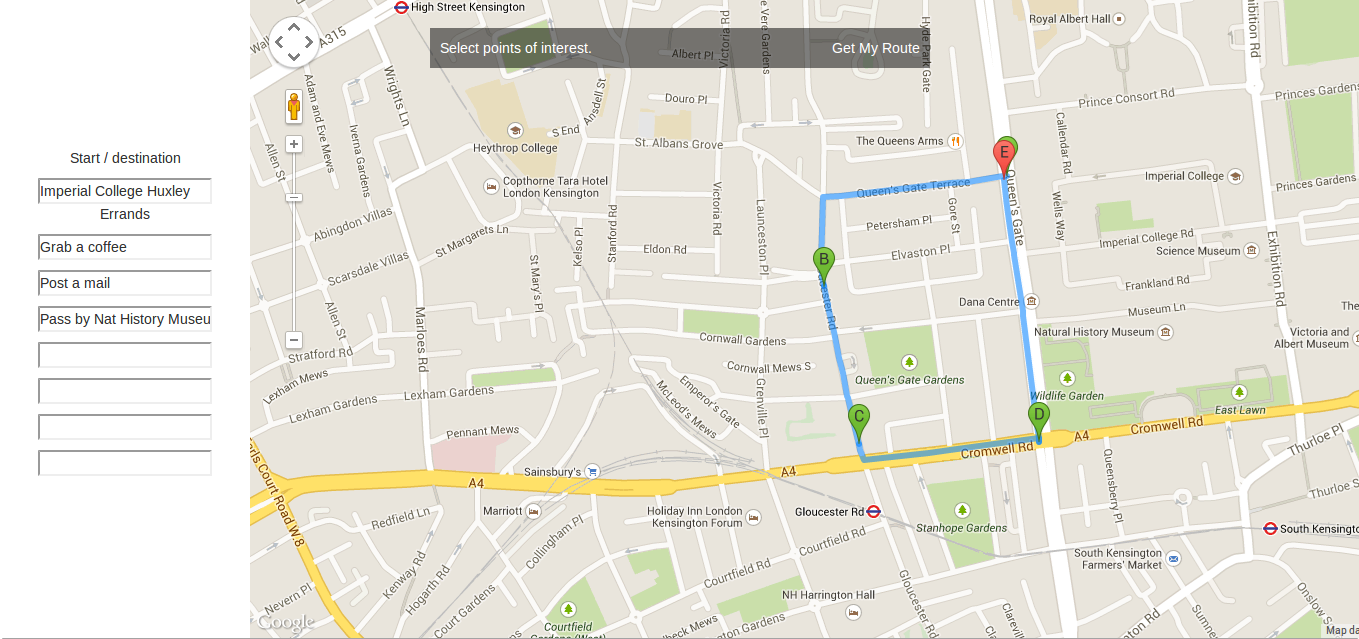
\includegraphics[scale=0.3]{hallway_q2.png}\\
Figure 23. UI the user will be presented with for this part of the test.
\end{center}

\chapter{User Interface Prototypes}
\begin{center}
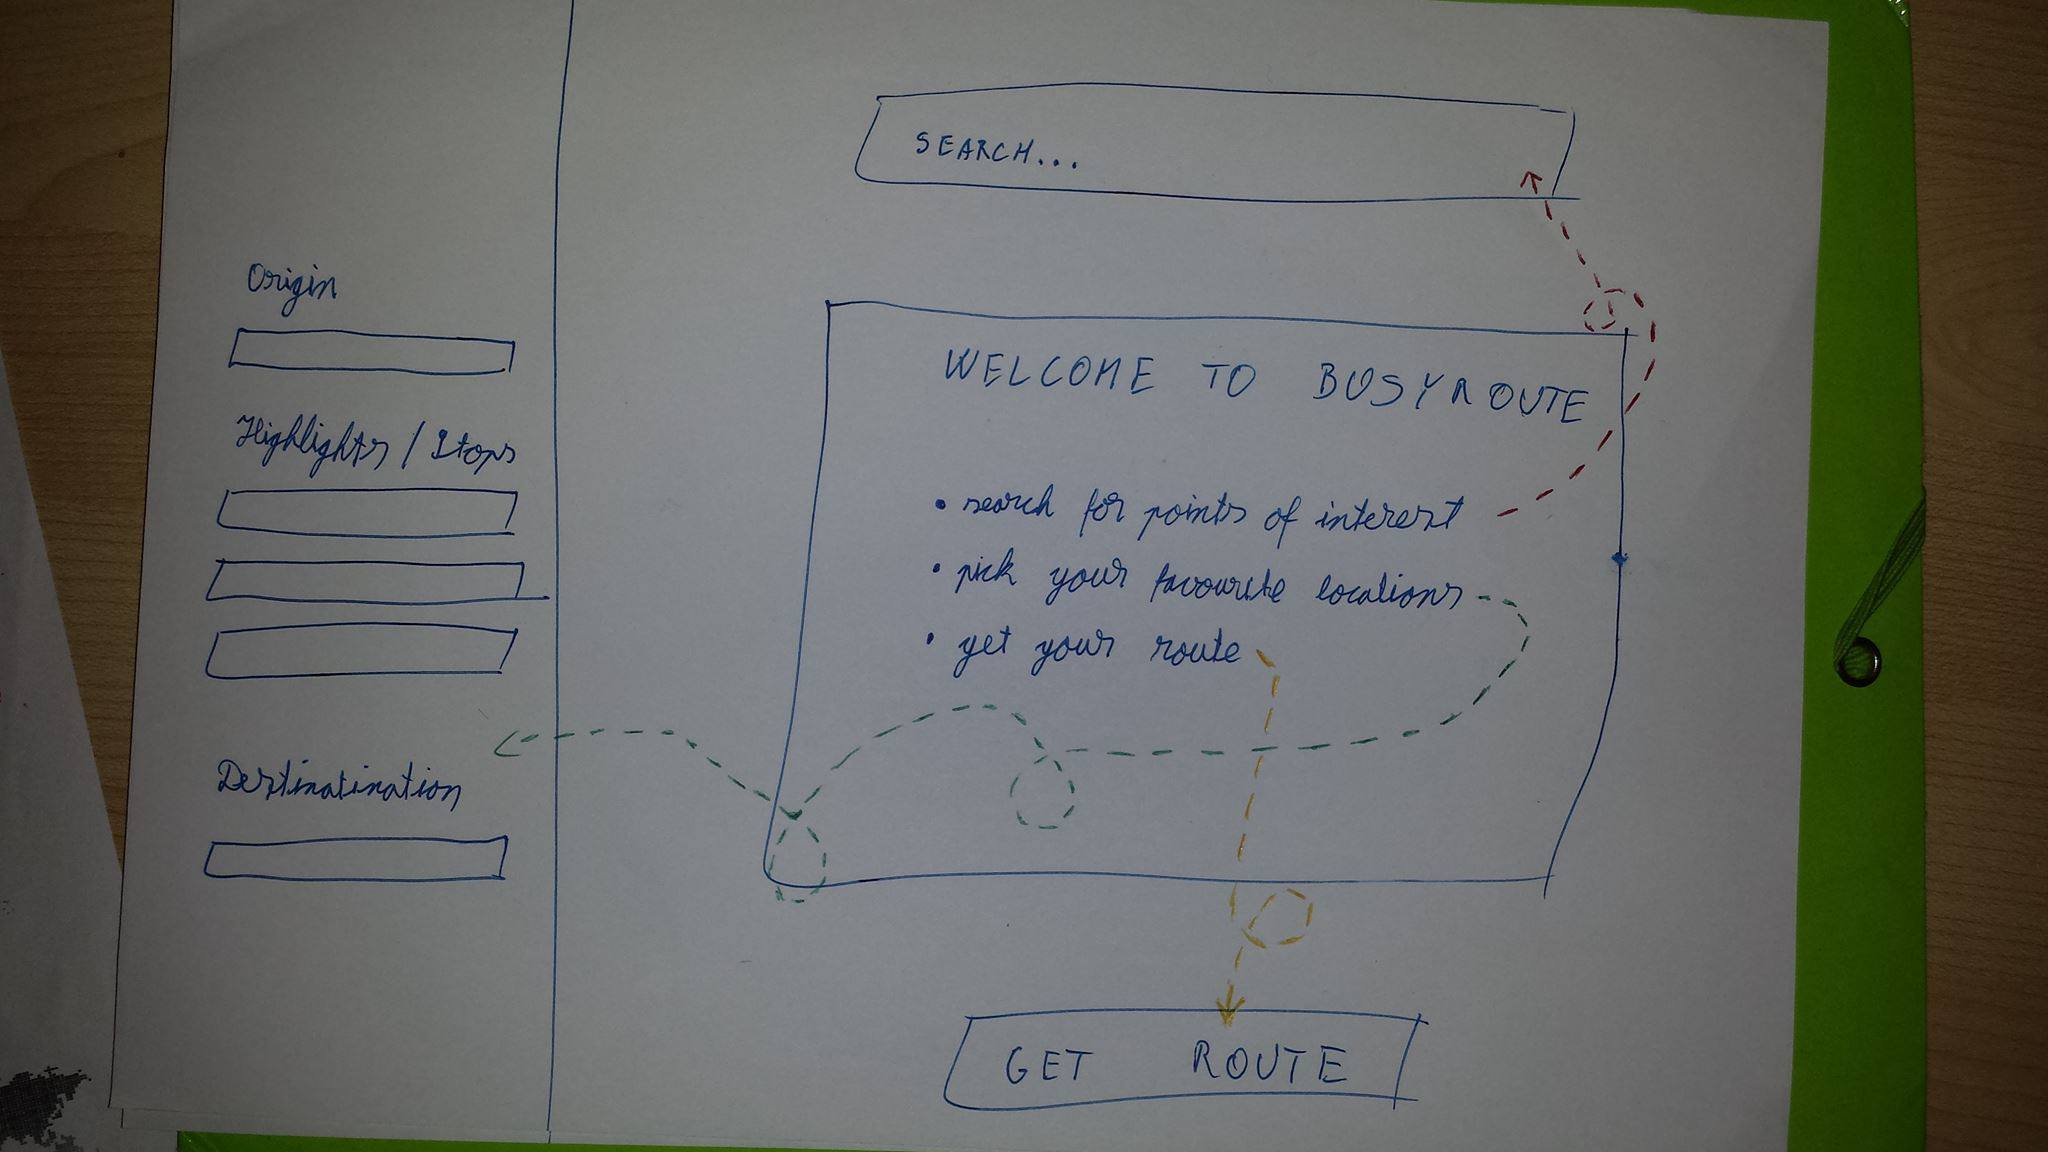
\includegraphics[scale=0.18]{proto_1.png}\\
Figure 24. Early paper prototype of the landing page.
\end{center}

\begin{center}
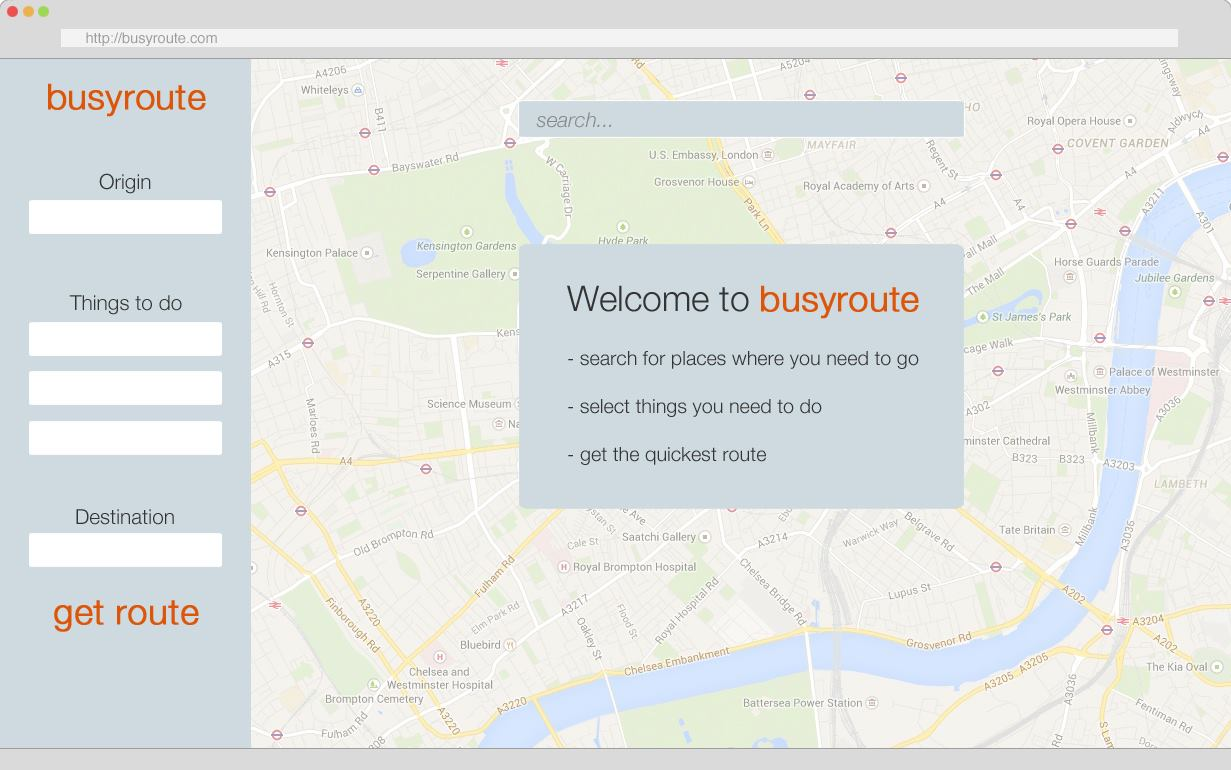
\includegraphics[scale=0.3]{proto_2.png}\\
Figure 25. Prototype of landing page.
\end{center}

\begin{center}
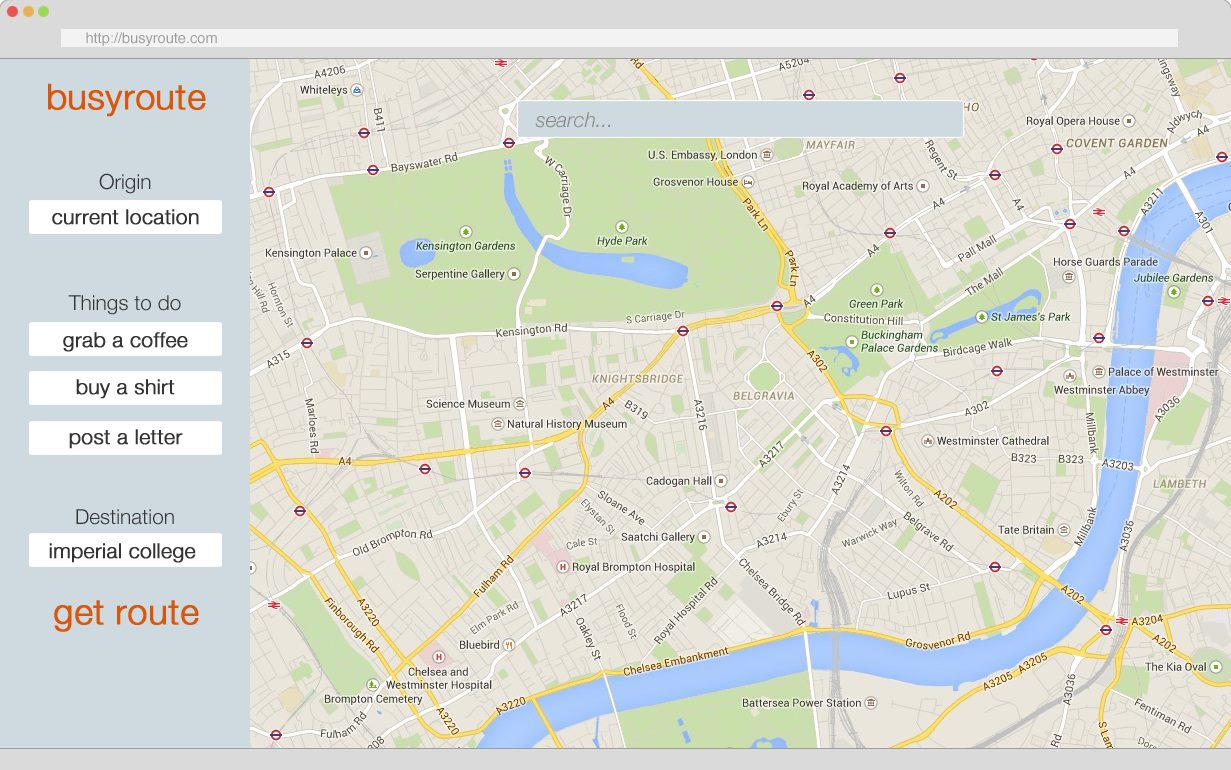
\includegraphics[scale=0.3]{proto_3.png}\\
Figure 26. Prototype of system whereby user enters his requirements.
\end{center}

\begin{center}
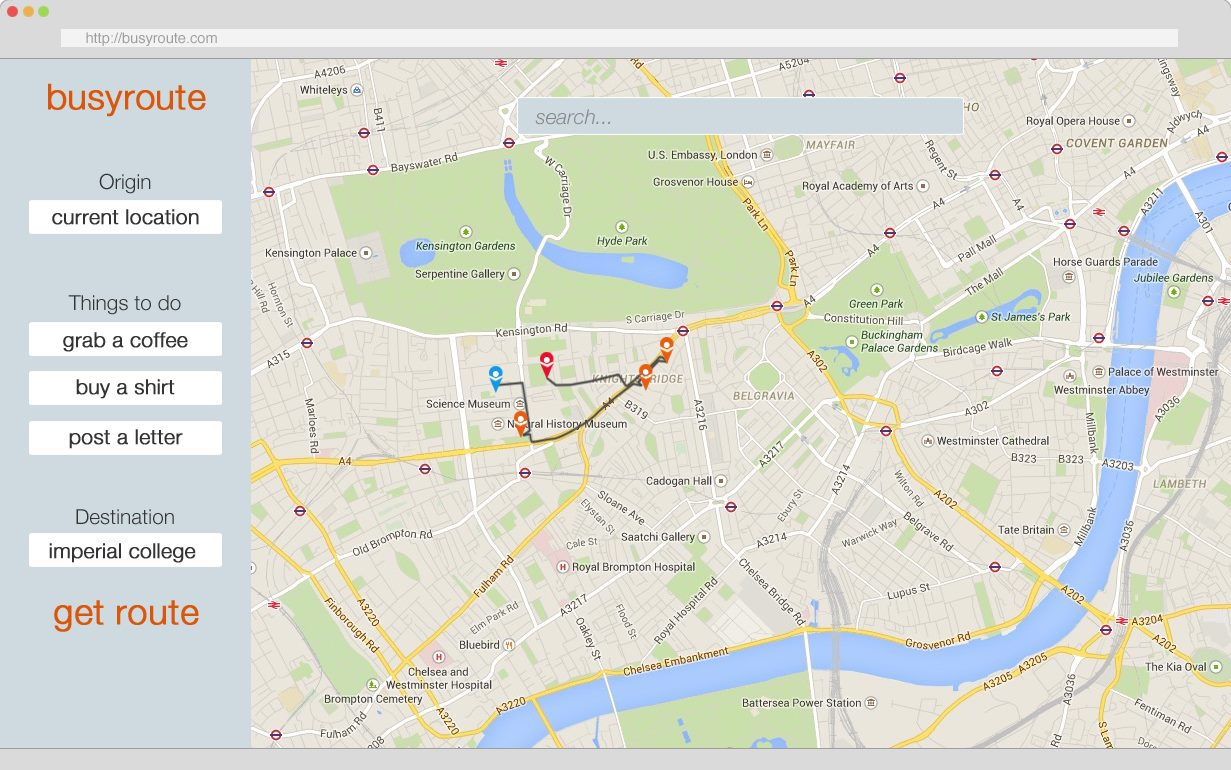
\includegraphics[scale=0.3]{proto_4.png}\\
Figure 27. Prototype of visualisation of the final route.
\end{center}

\chapter{User Manual}
\begin{center}
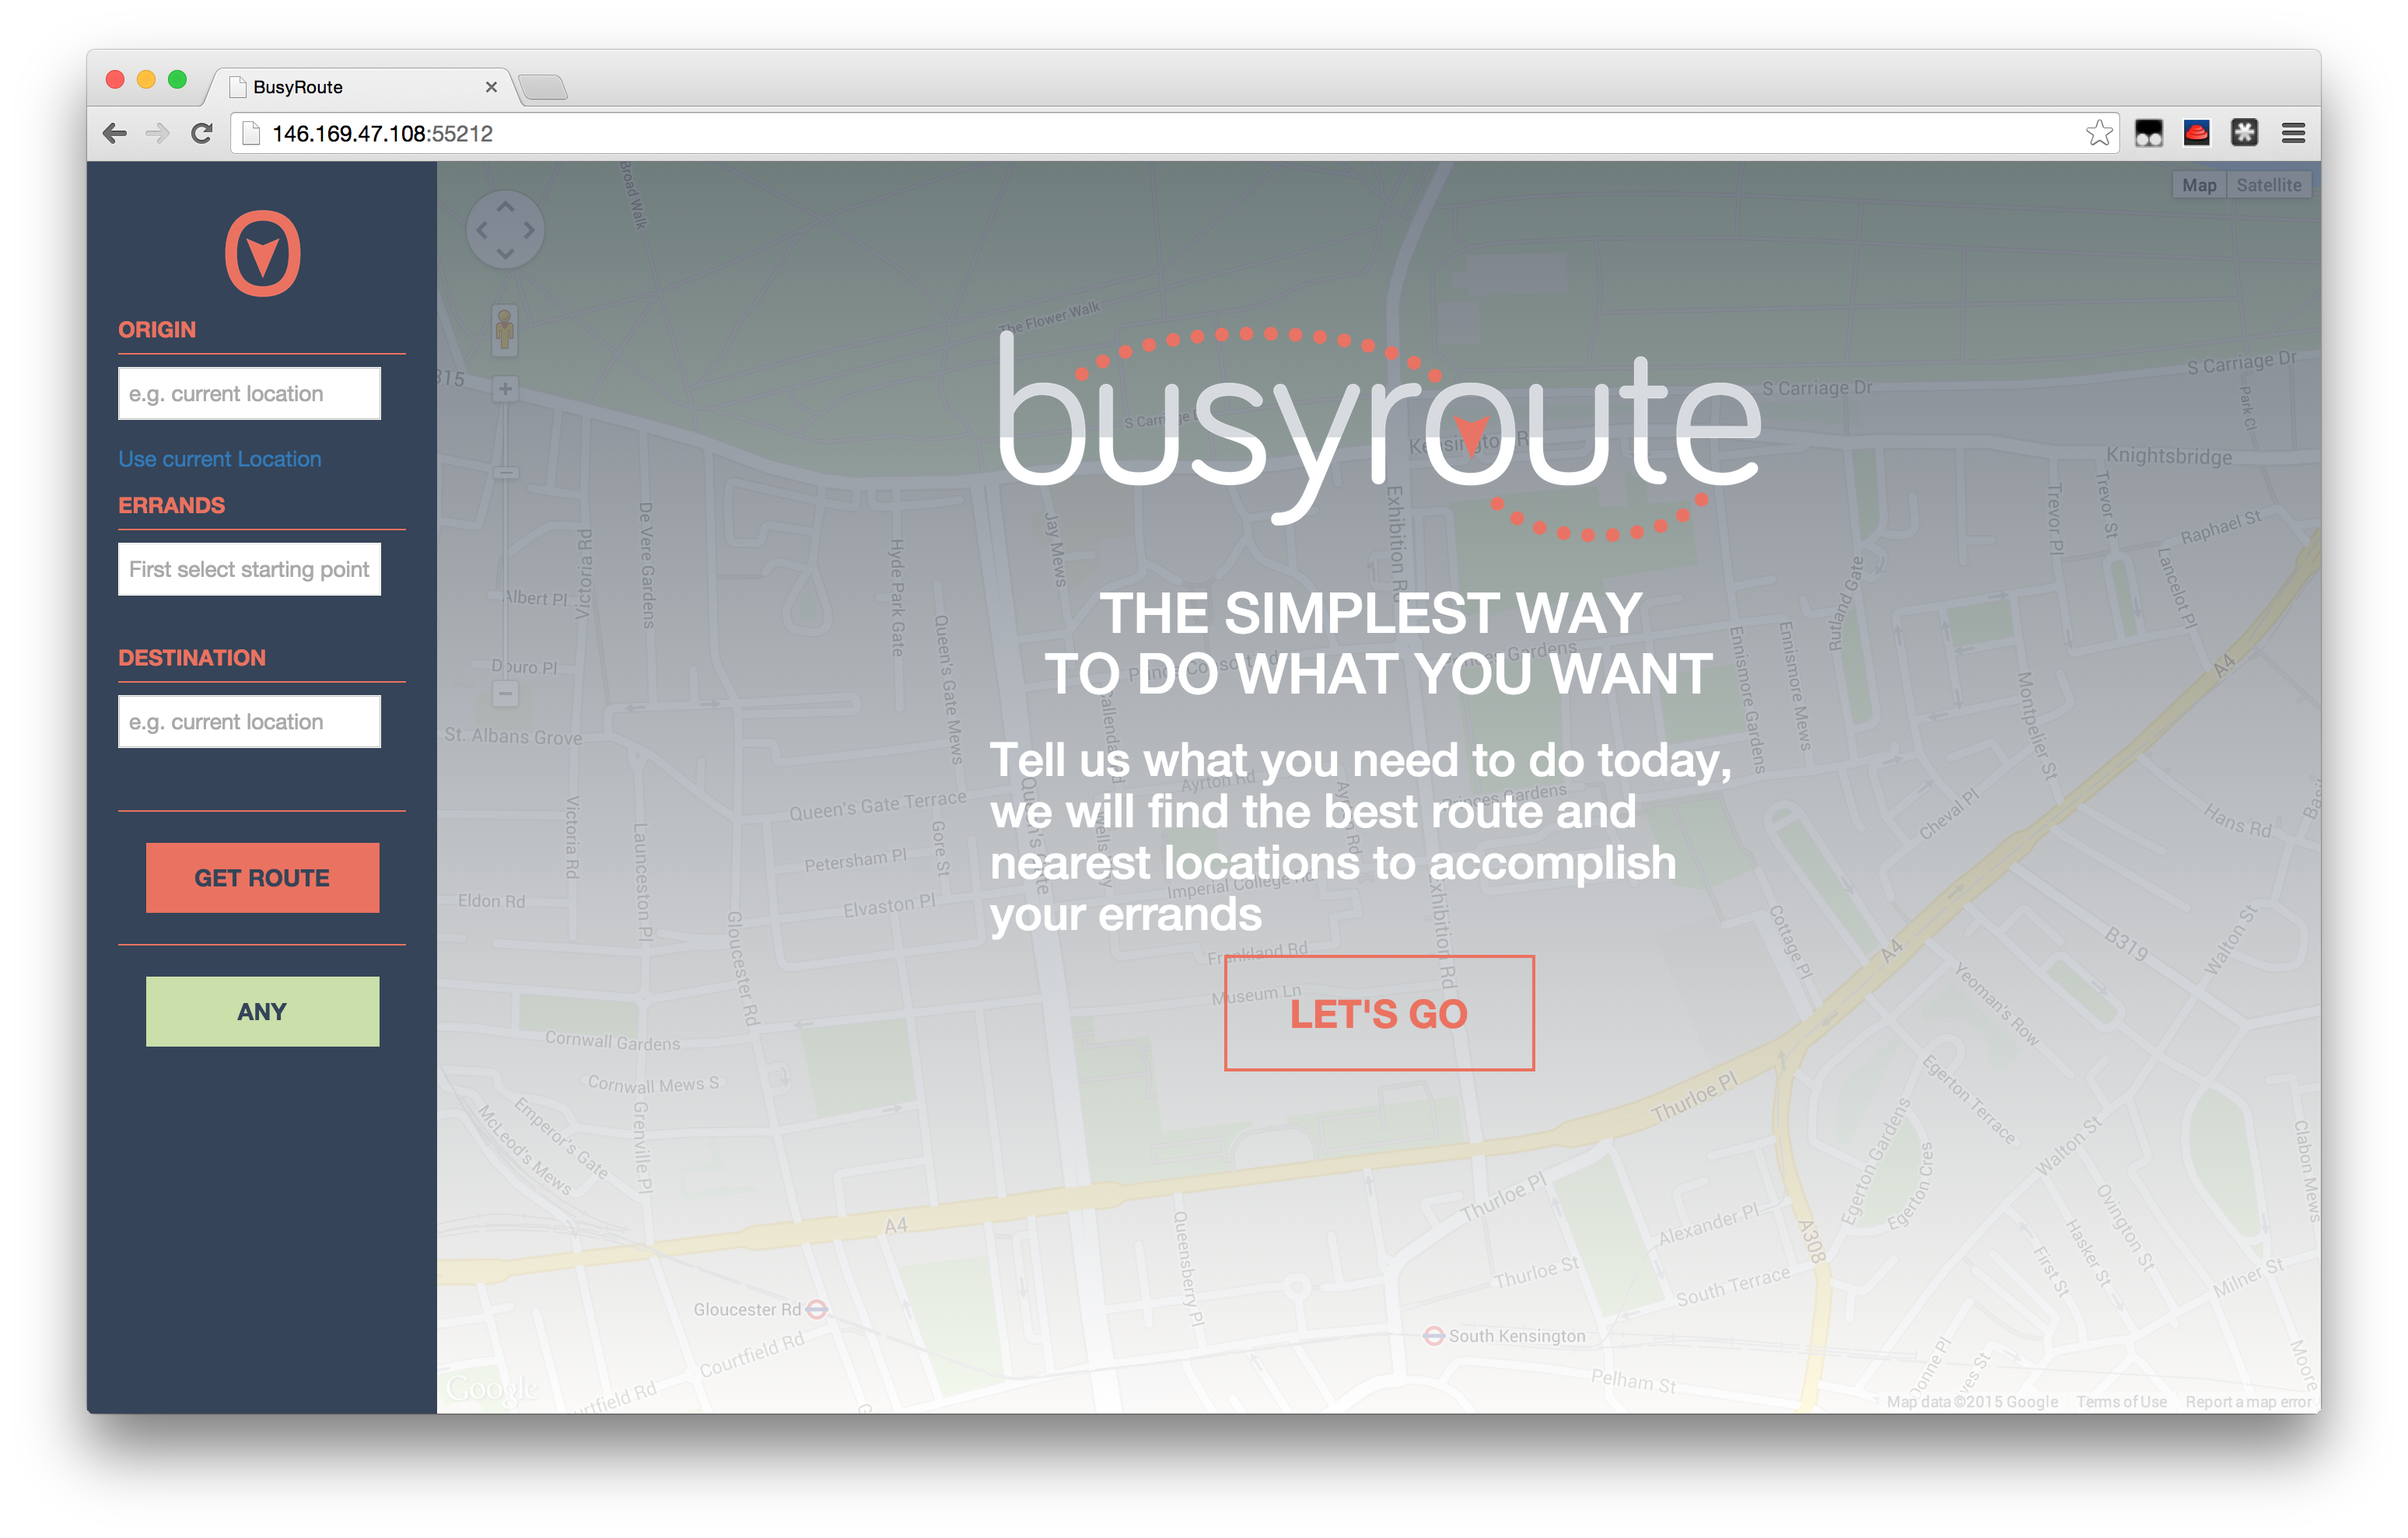
\includegraphics[scale=0.18]{um-01-starting.png}\\
Figure 28. Click ``Let's Go" to begin.
\end{center}
\begin{center}
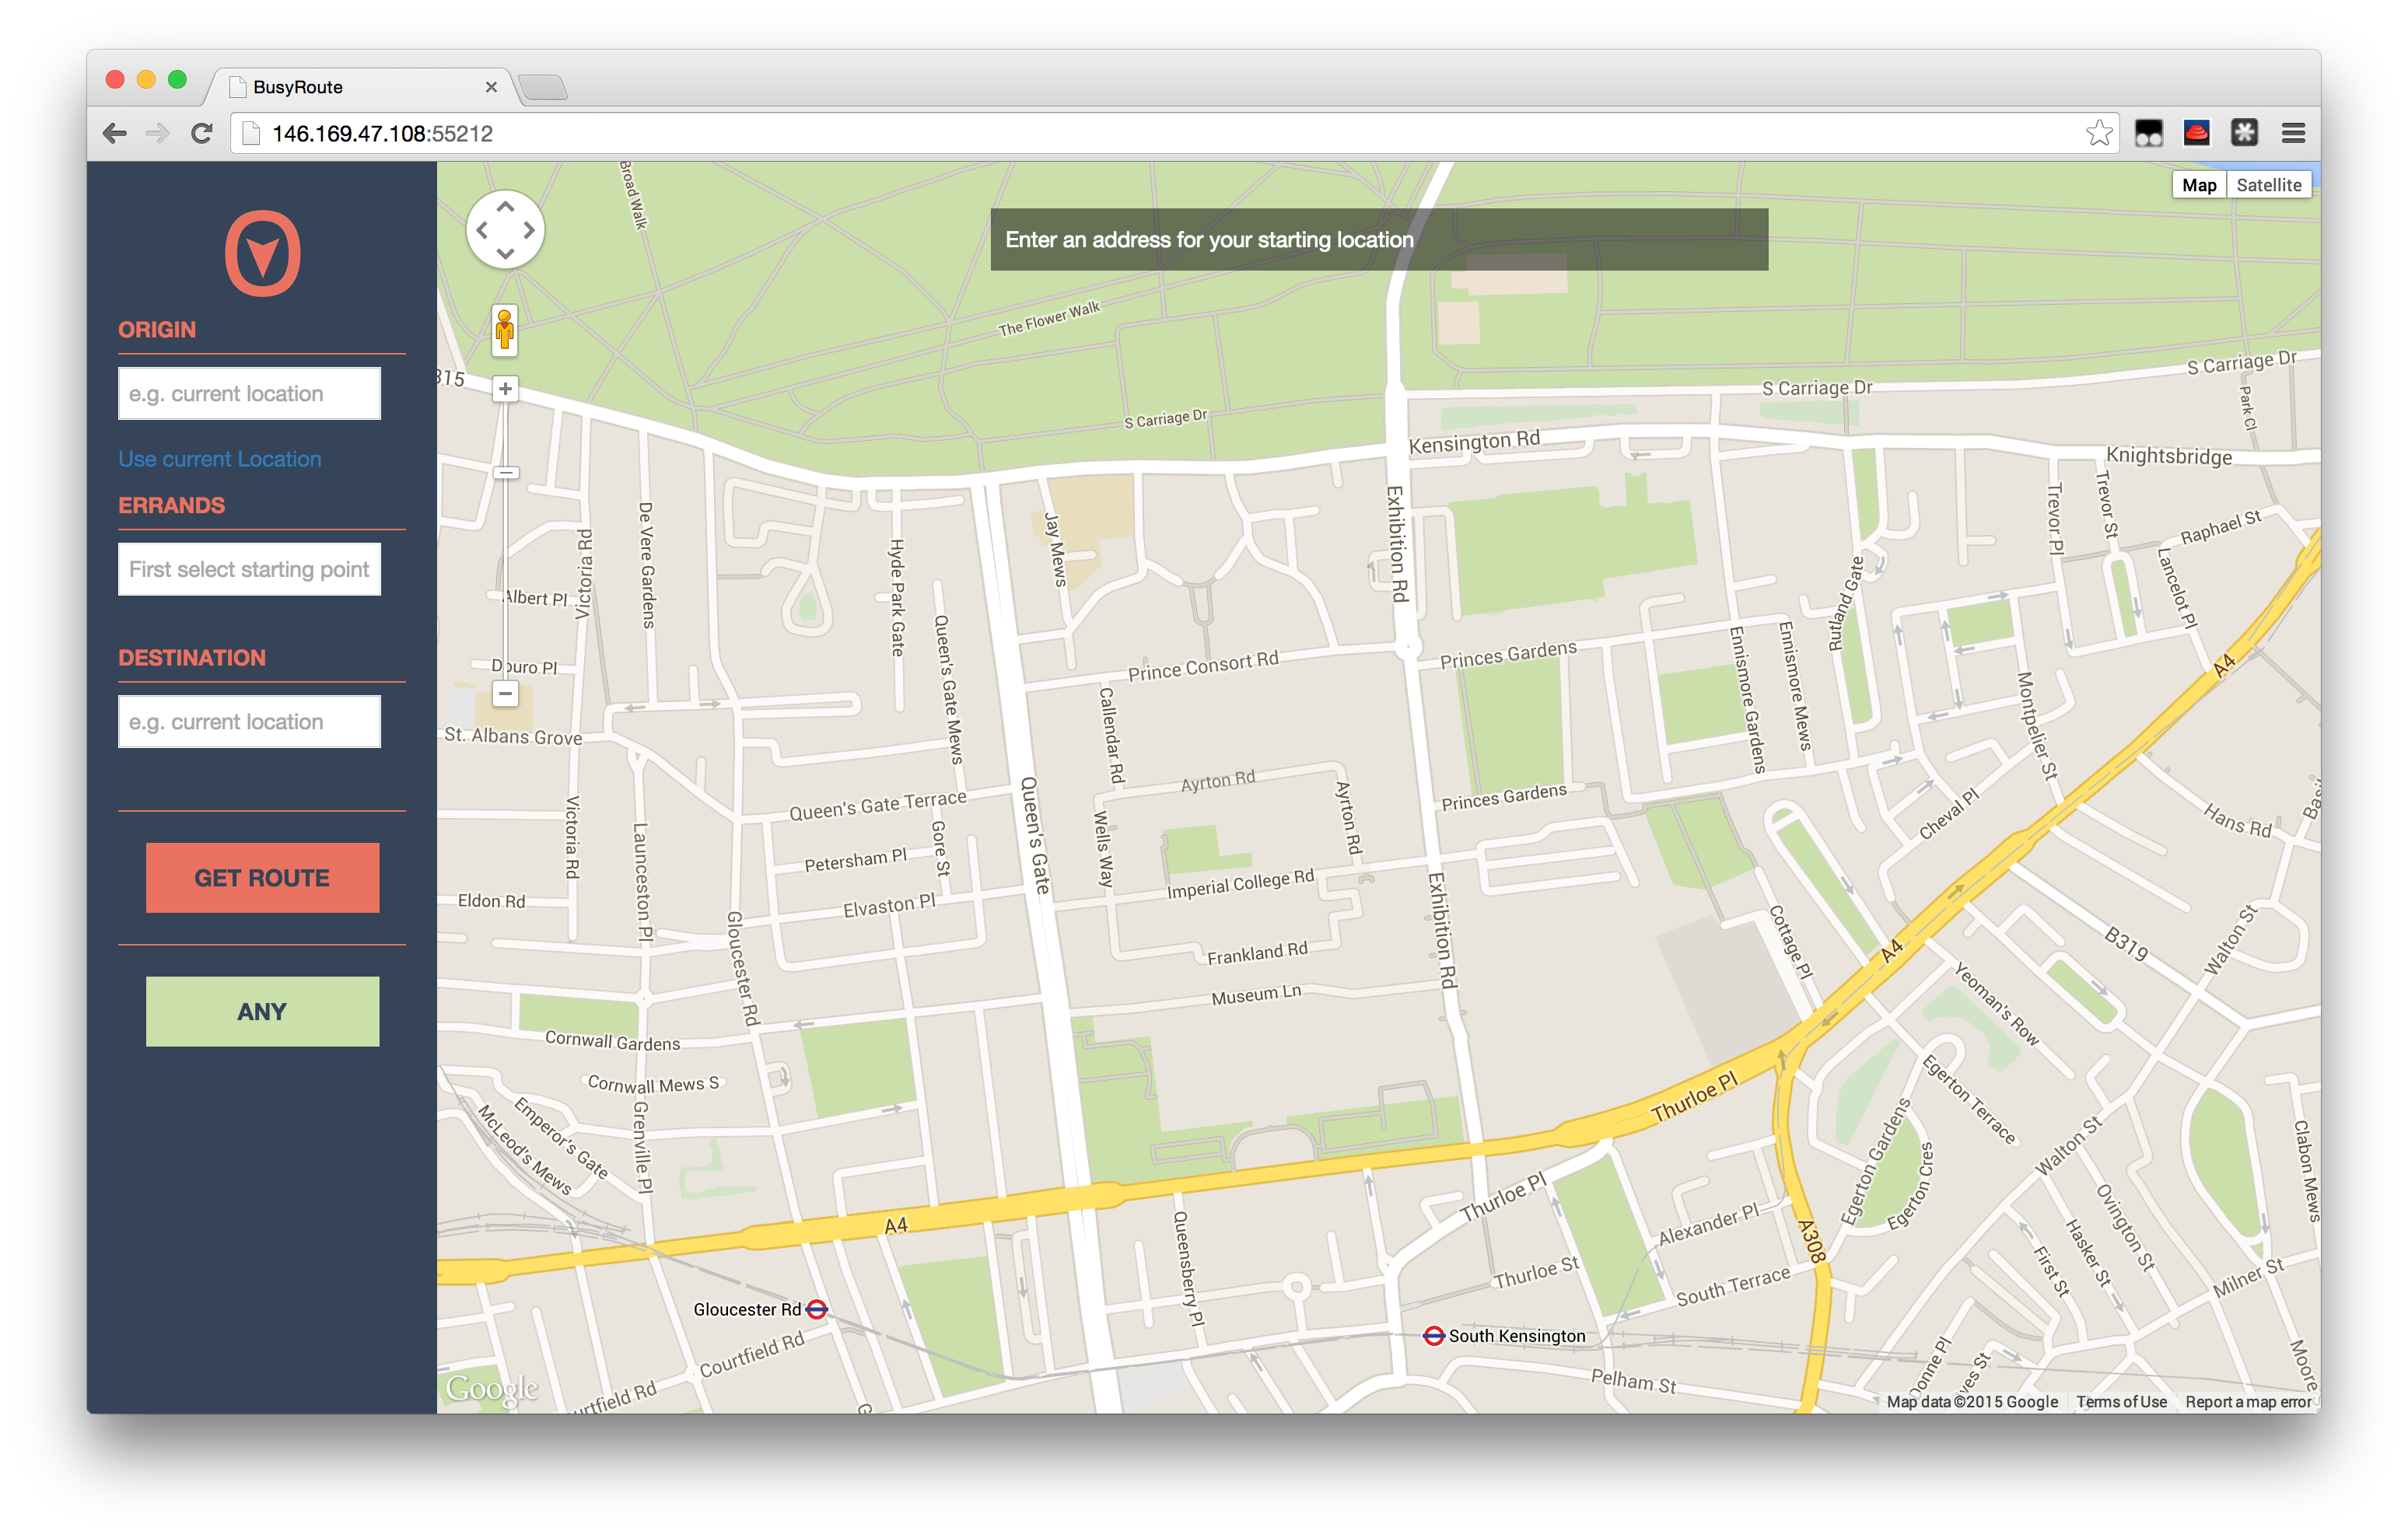
\includegraphics[scale=0.18]{um-02-clean.png}\\
Figure 29. Pan map canvas to point of interest.
\end{center}
\begin{center}
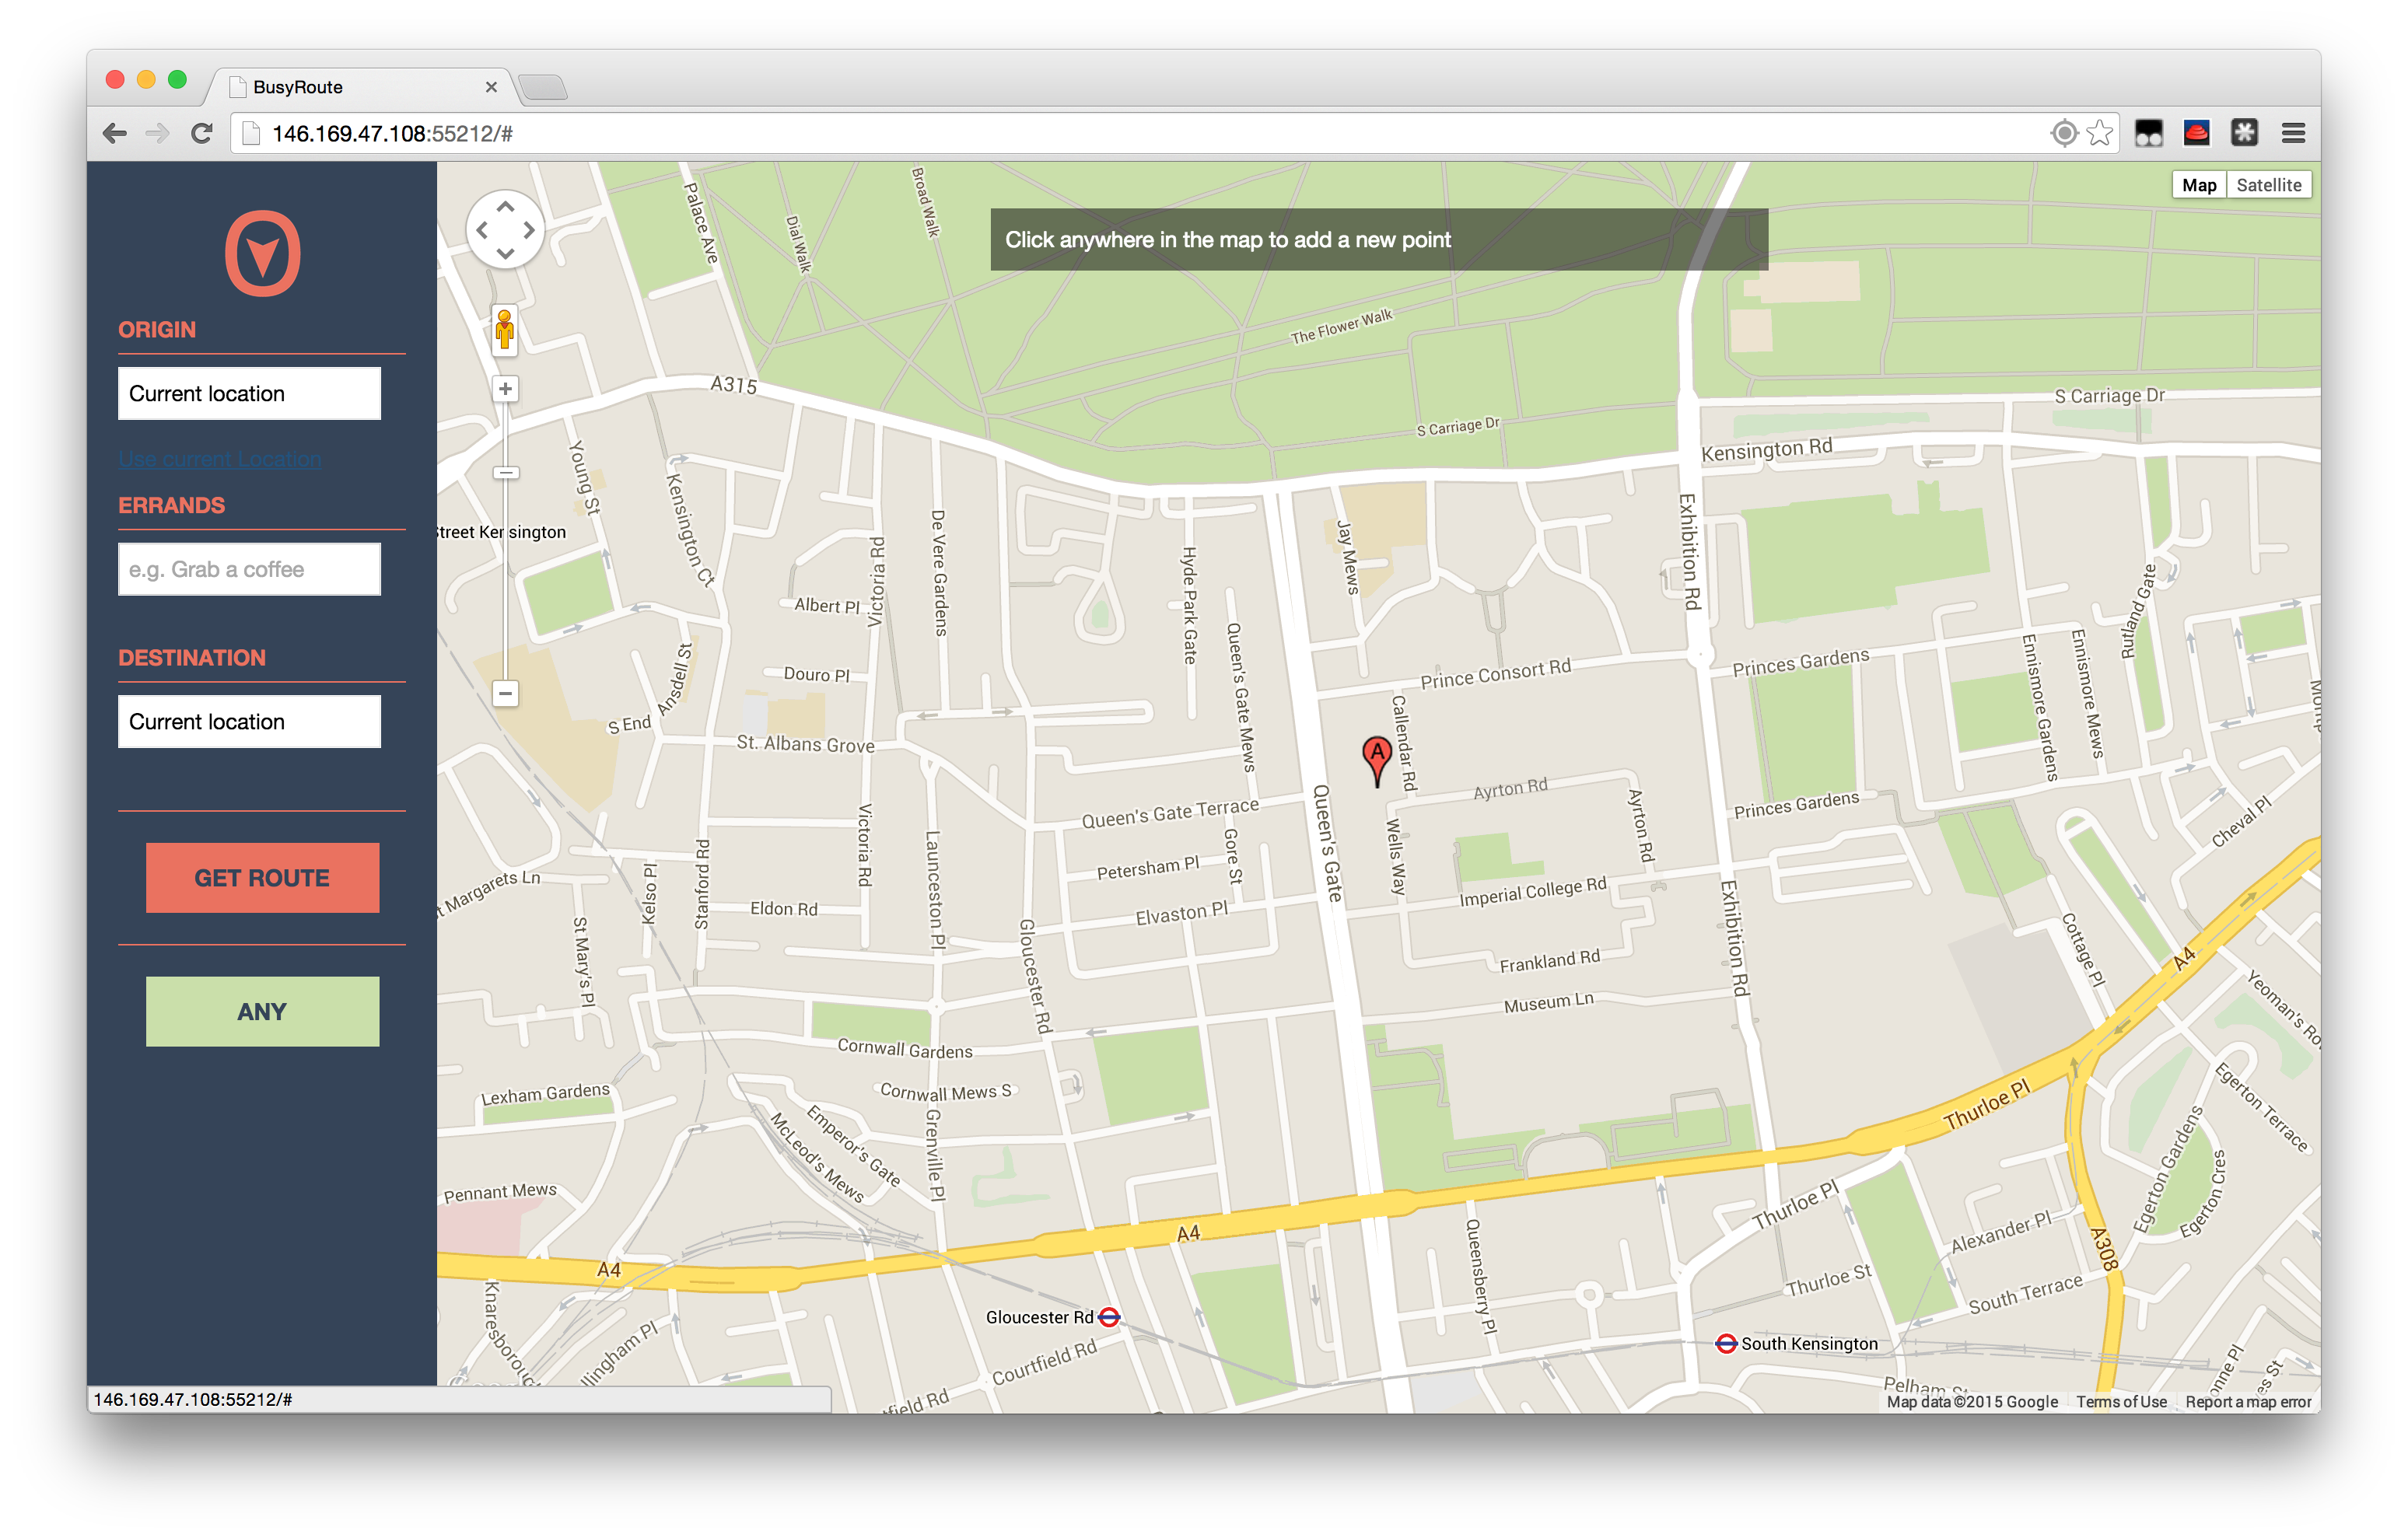
\includegraphics[scale=0.18]{um-03-current-loc.png}\\
Figure 30. Set starting location with pin drop or current location.
\end{center}
\begin{center}
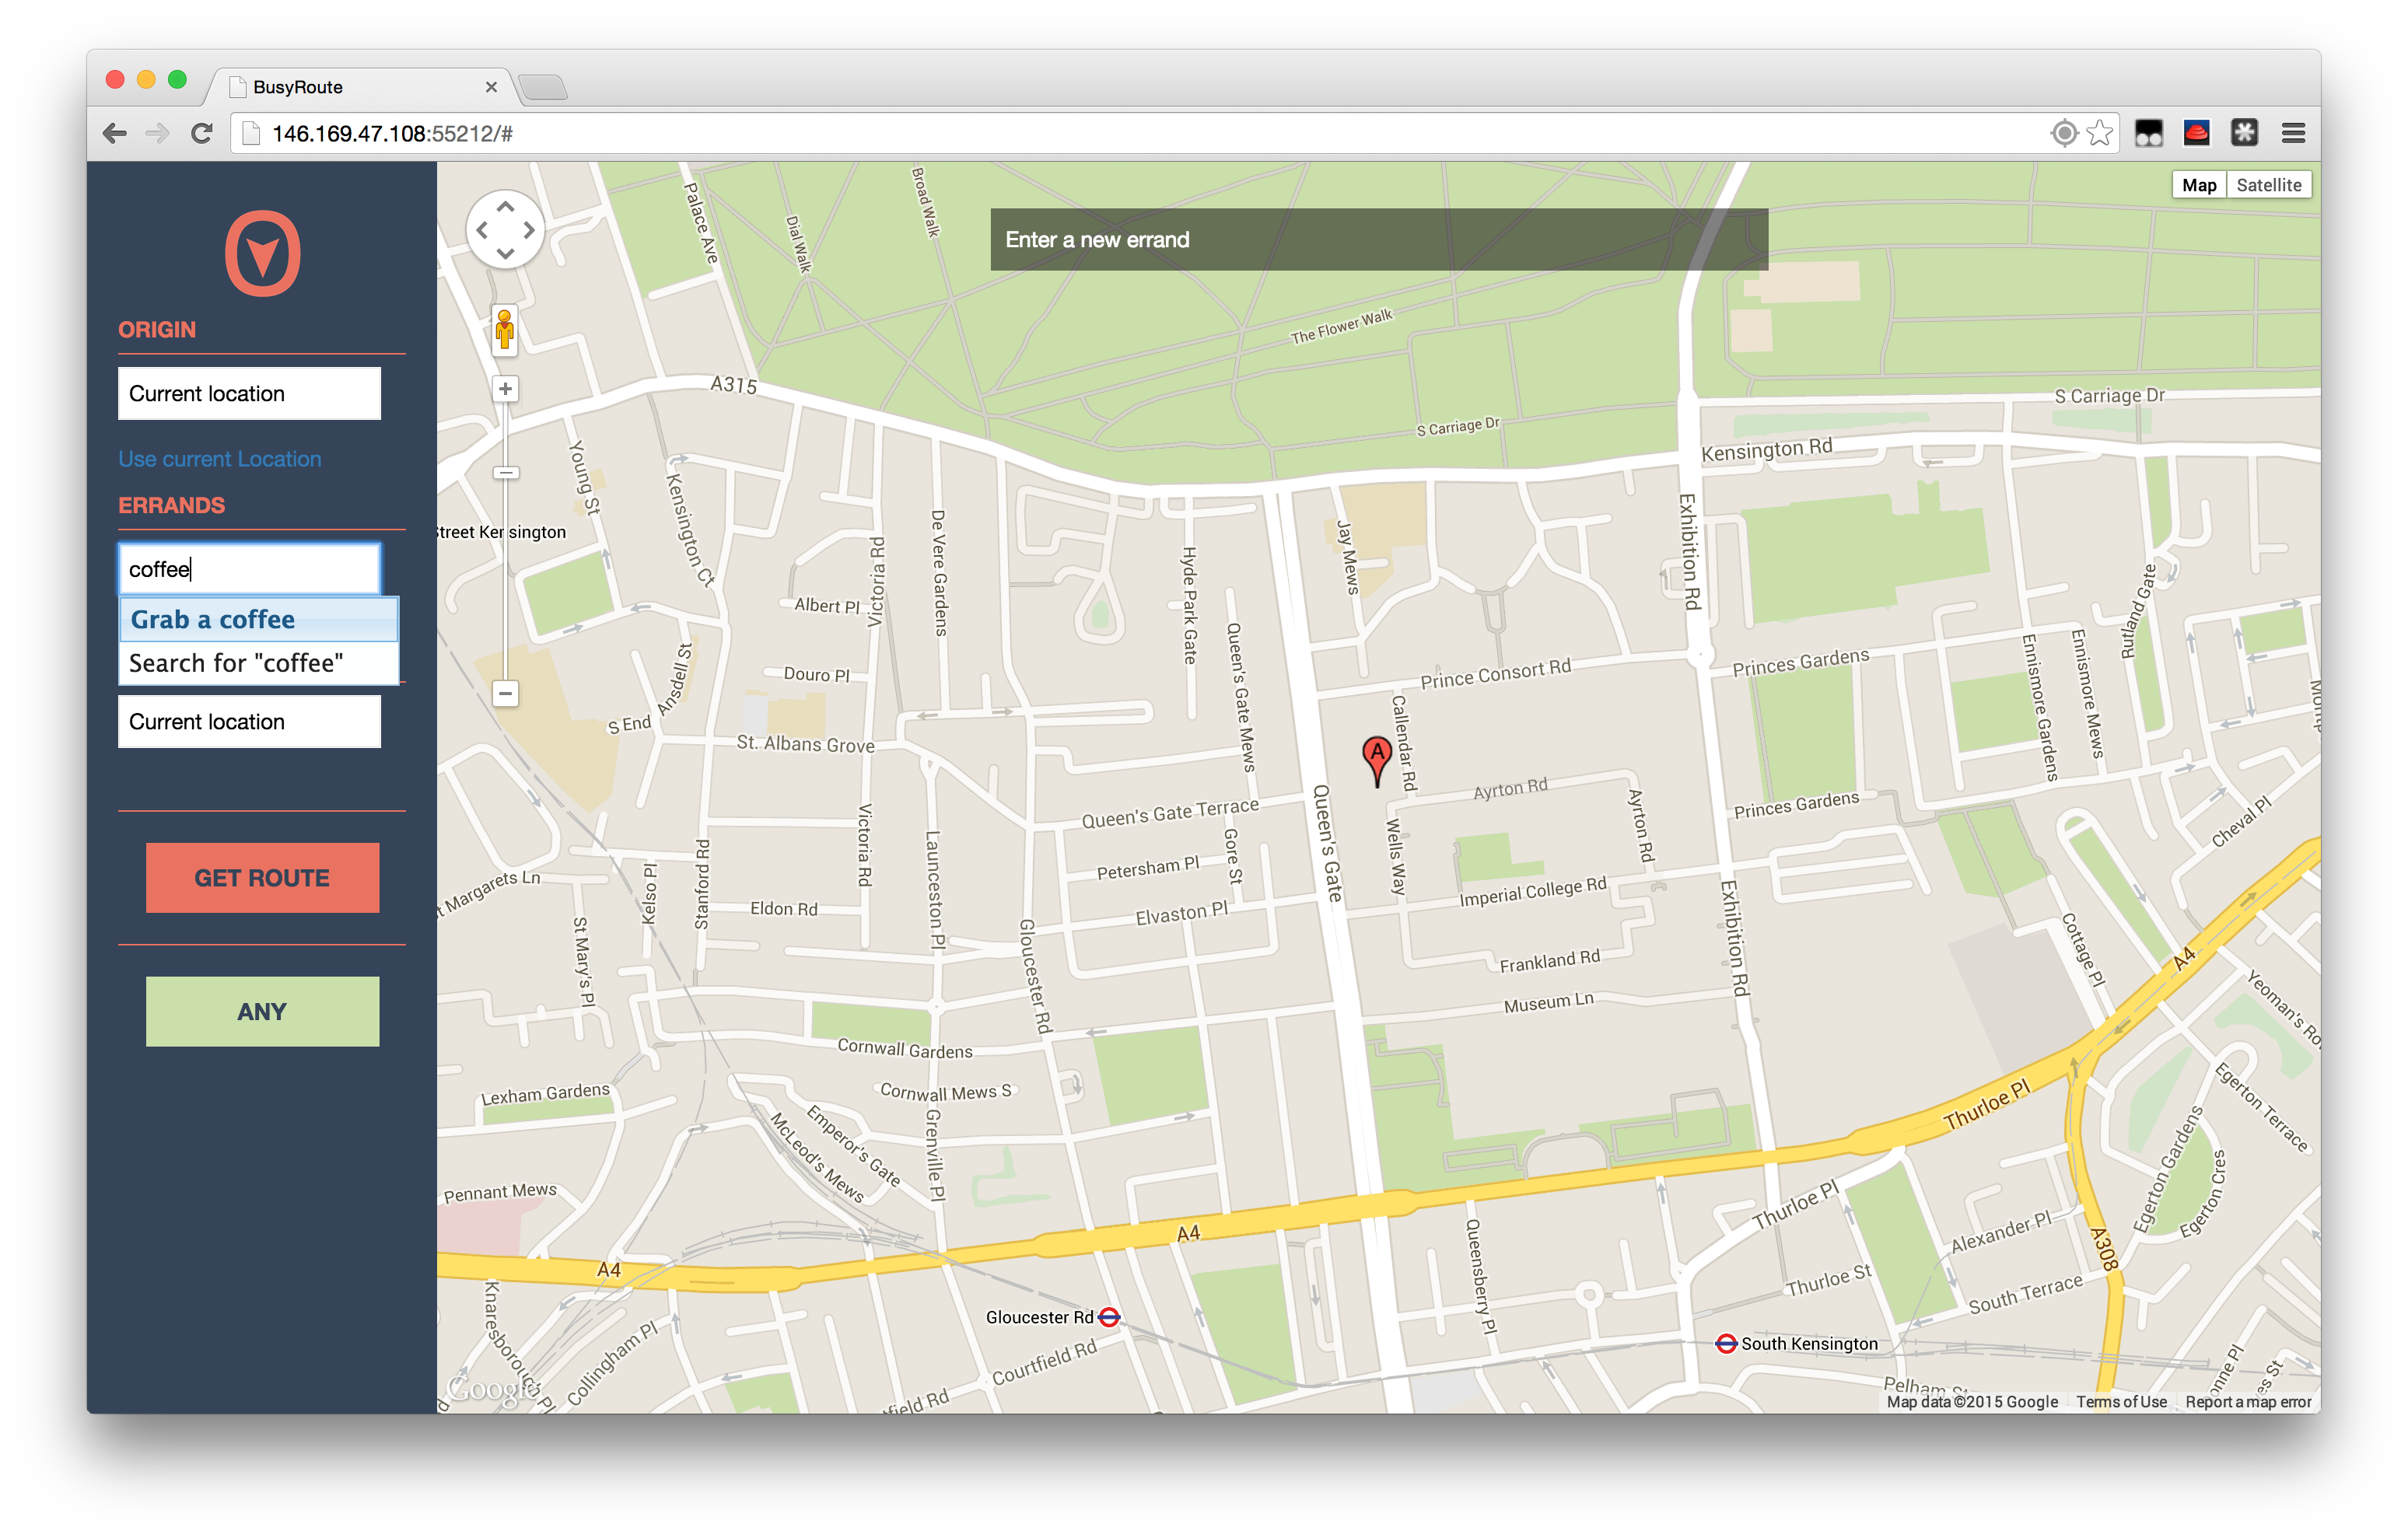
\includegraphics[scale=0.18]{um-04-search-errand.png}\\
Figure 31. Search keywords for supported errand.
\end{center}
\begin{center}
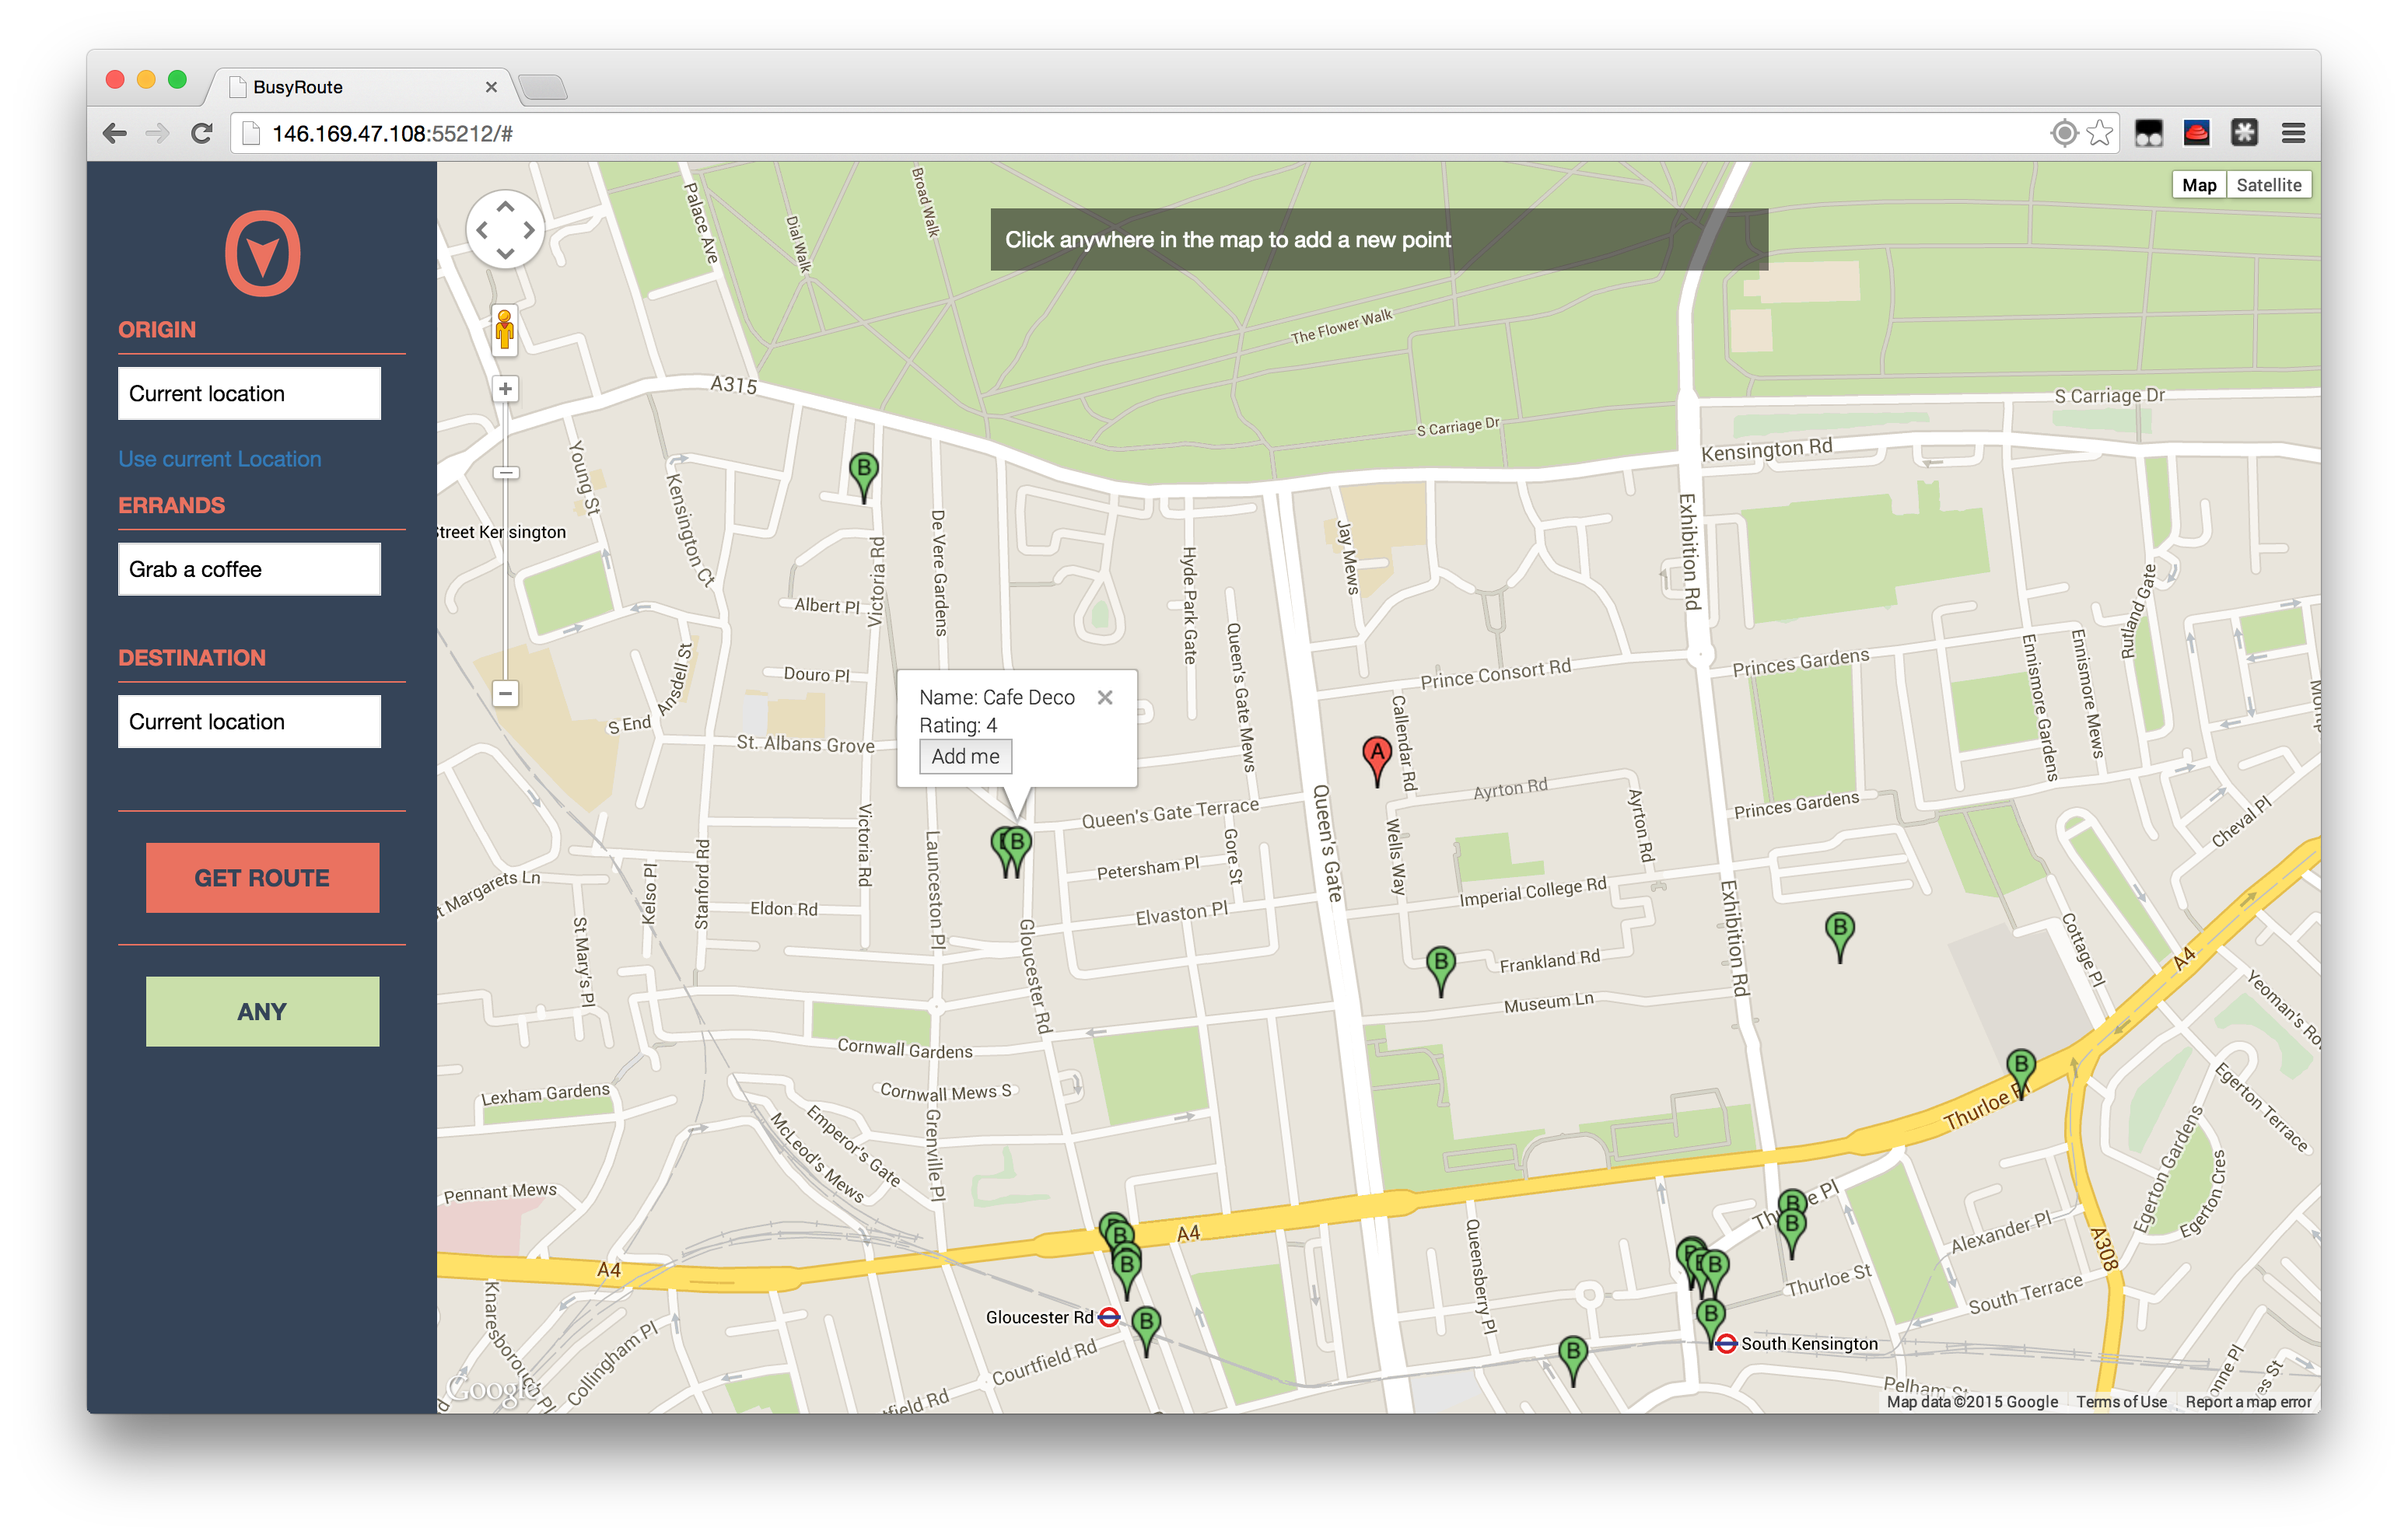
\includegraphics[scale=0.18]{um-05-place-detail.png}\\
Figure 32. Browse possible locations for errand completion.
\end{center}
\begin{center}
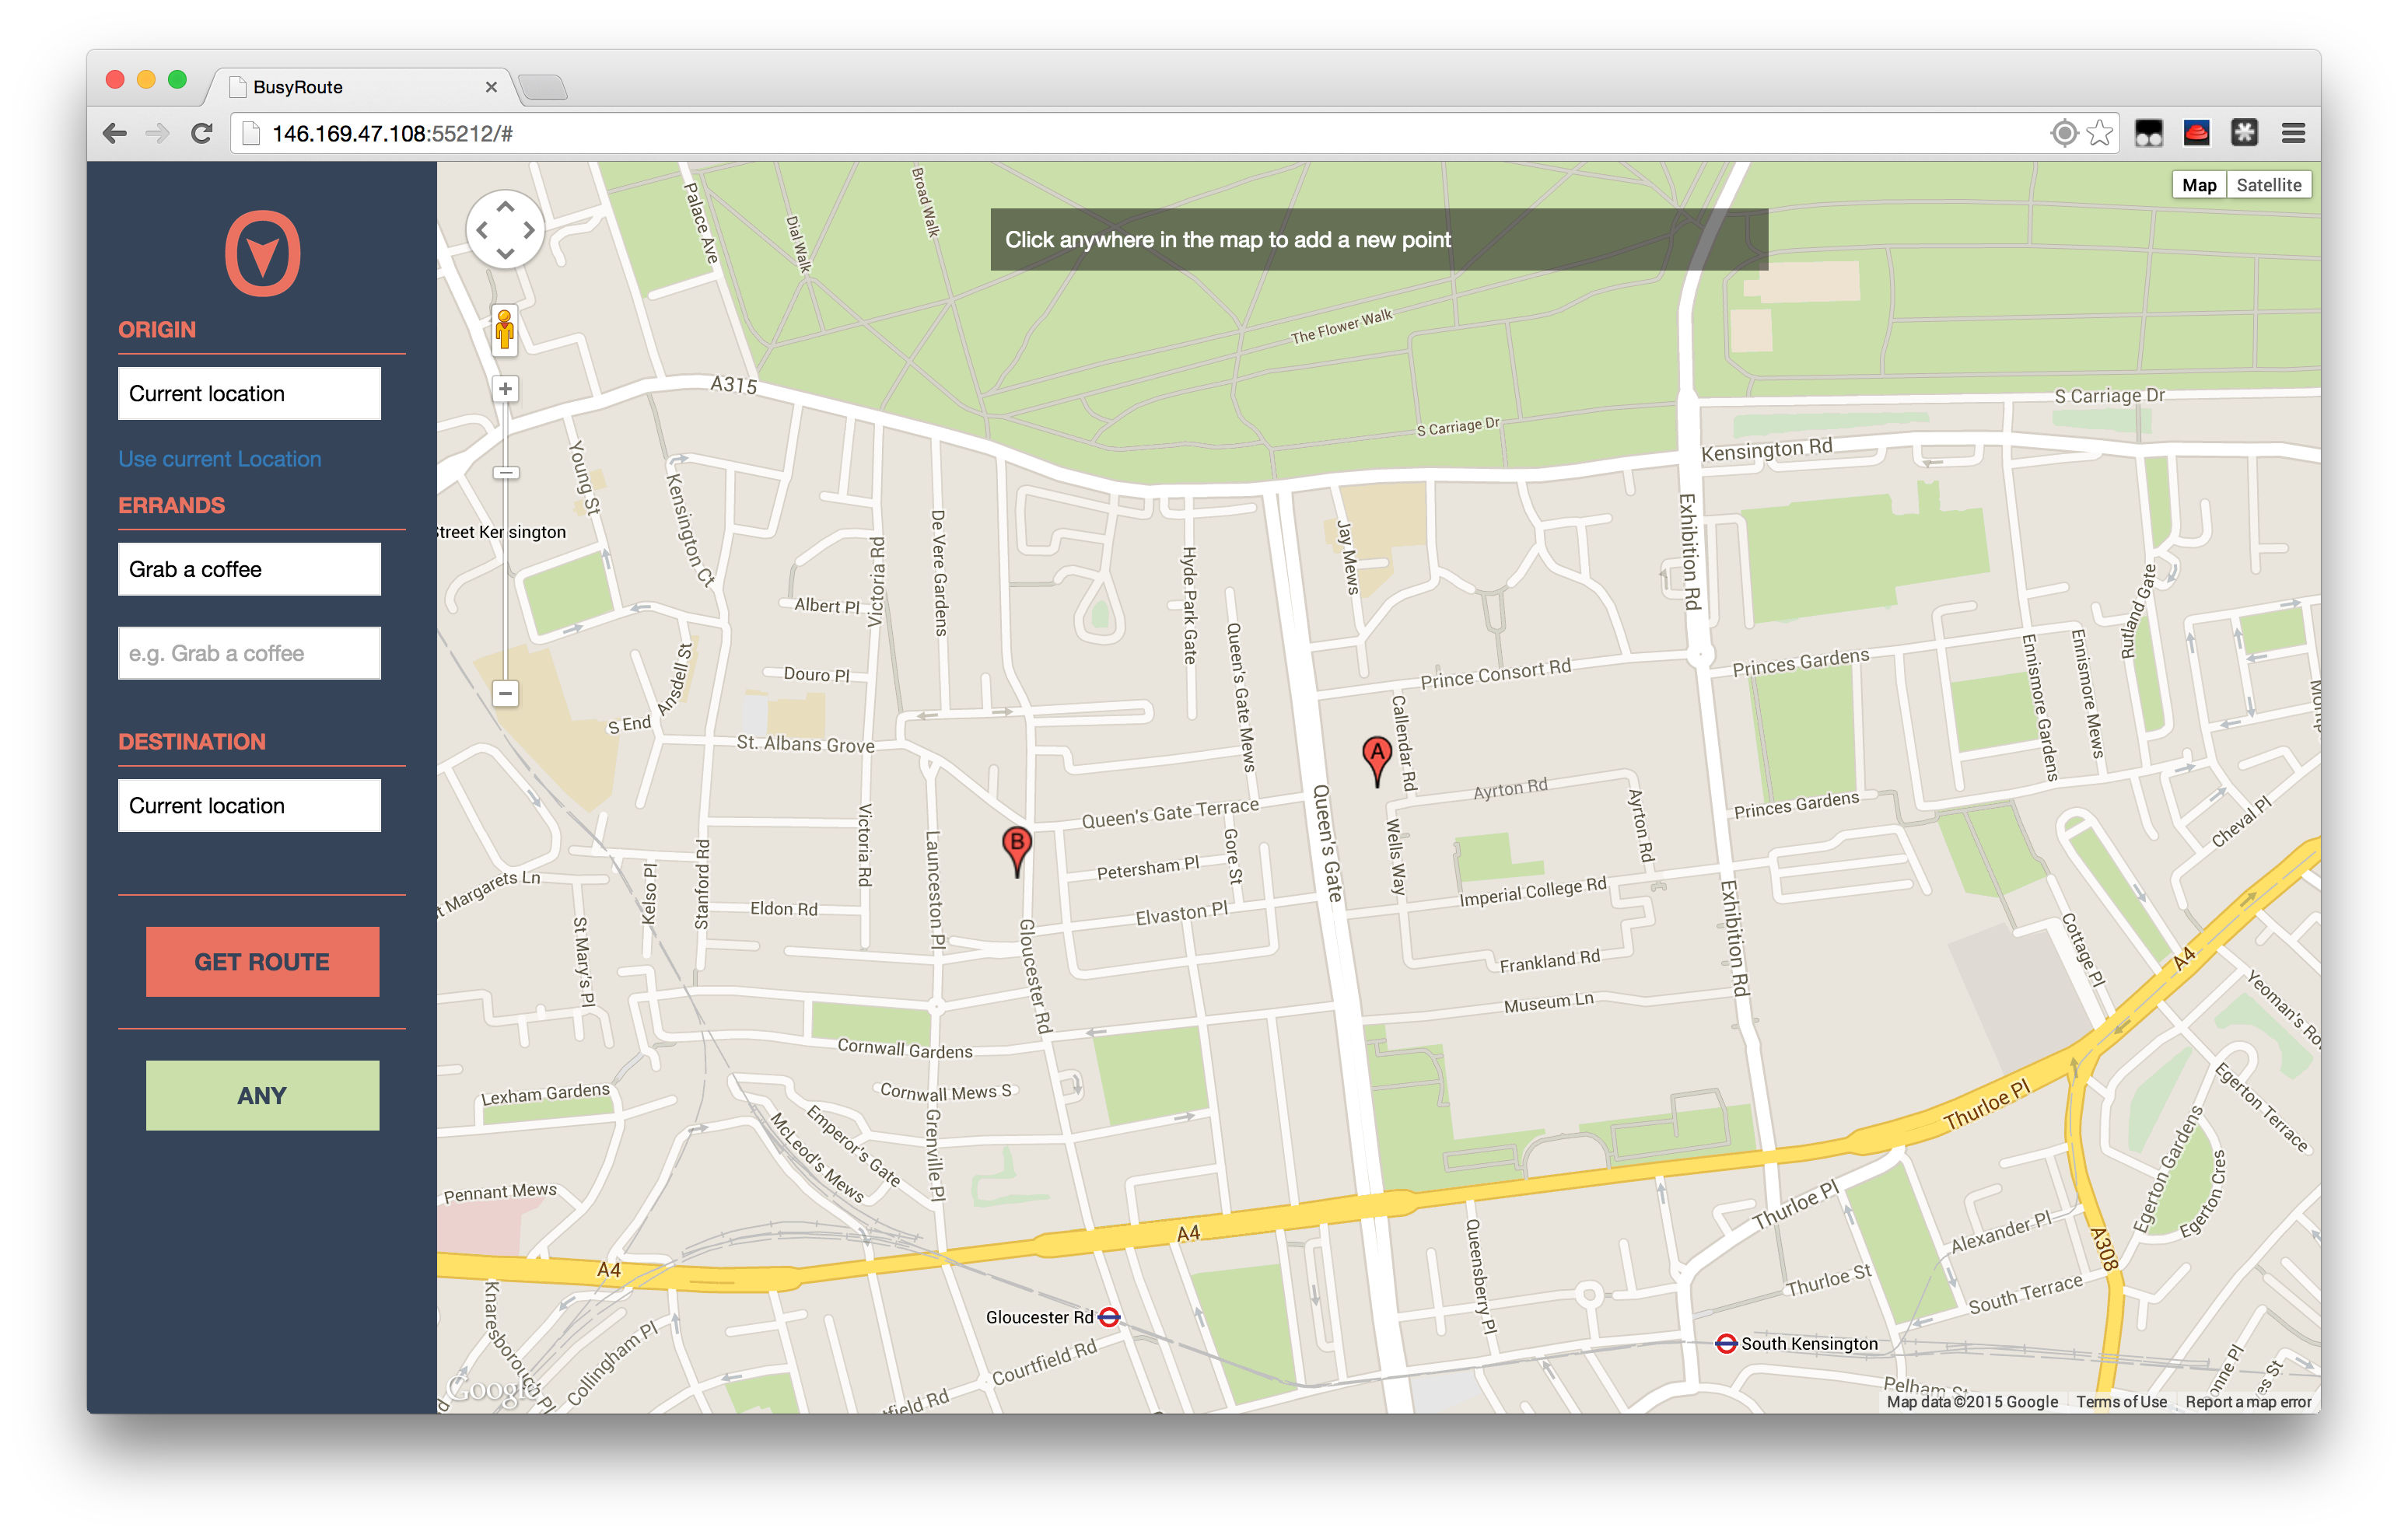
\includegraphics[scale=0.18]{um-06-place-select.png}\\
Figure 33. Screen after choosing suitable location for errand (click ``Add me").
\end{center}
\begin{center}
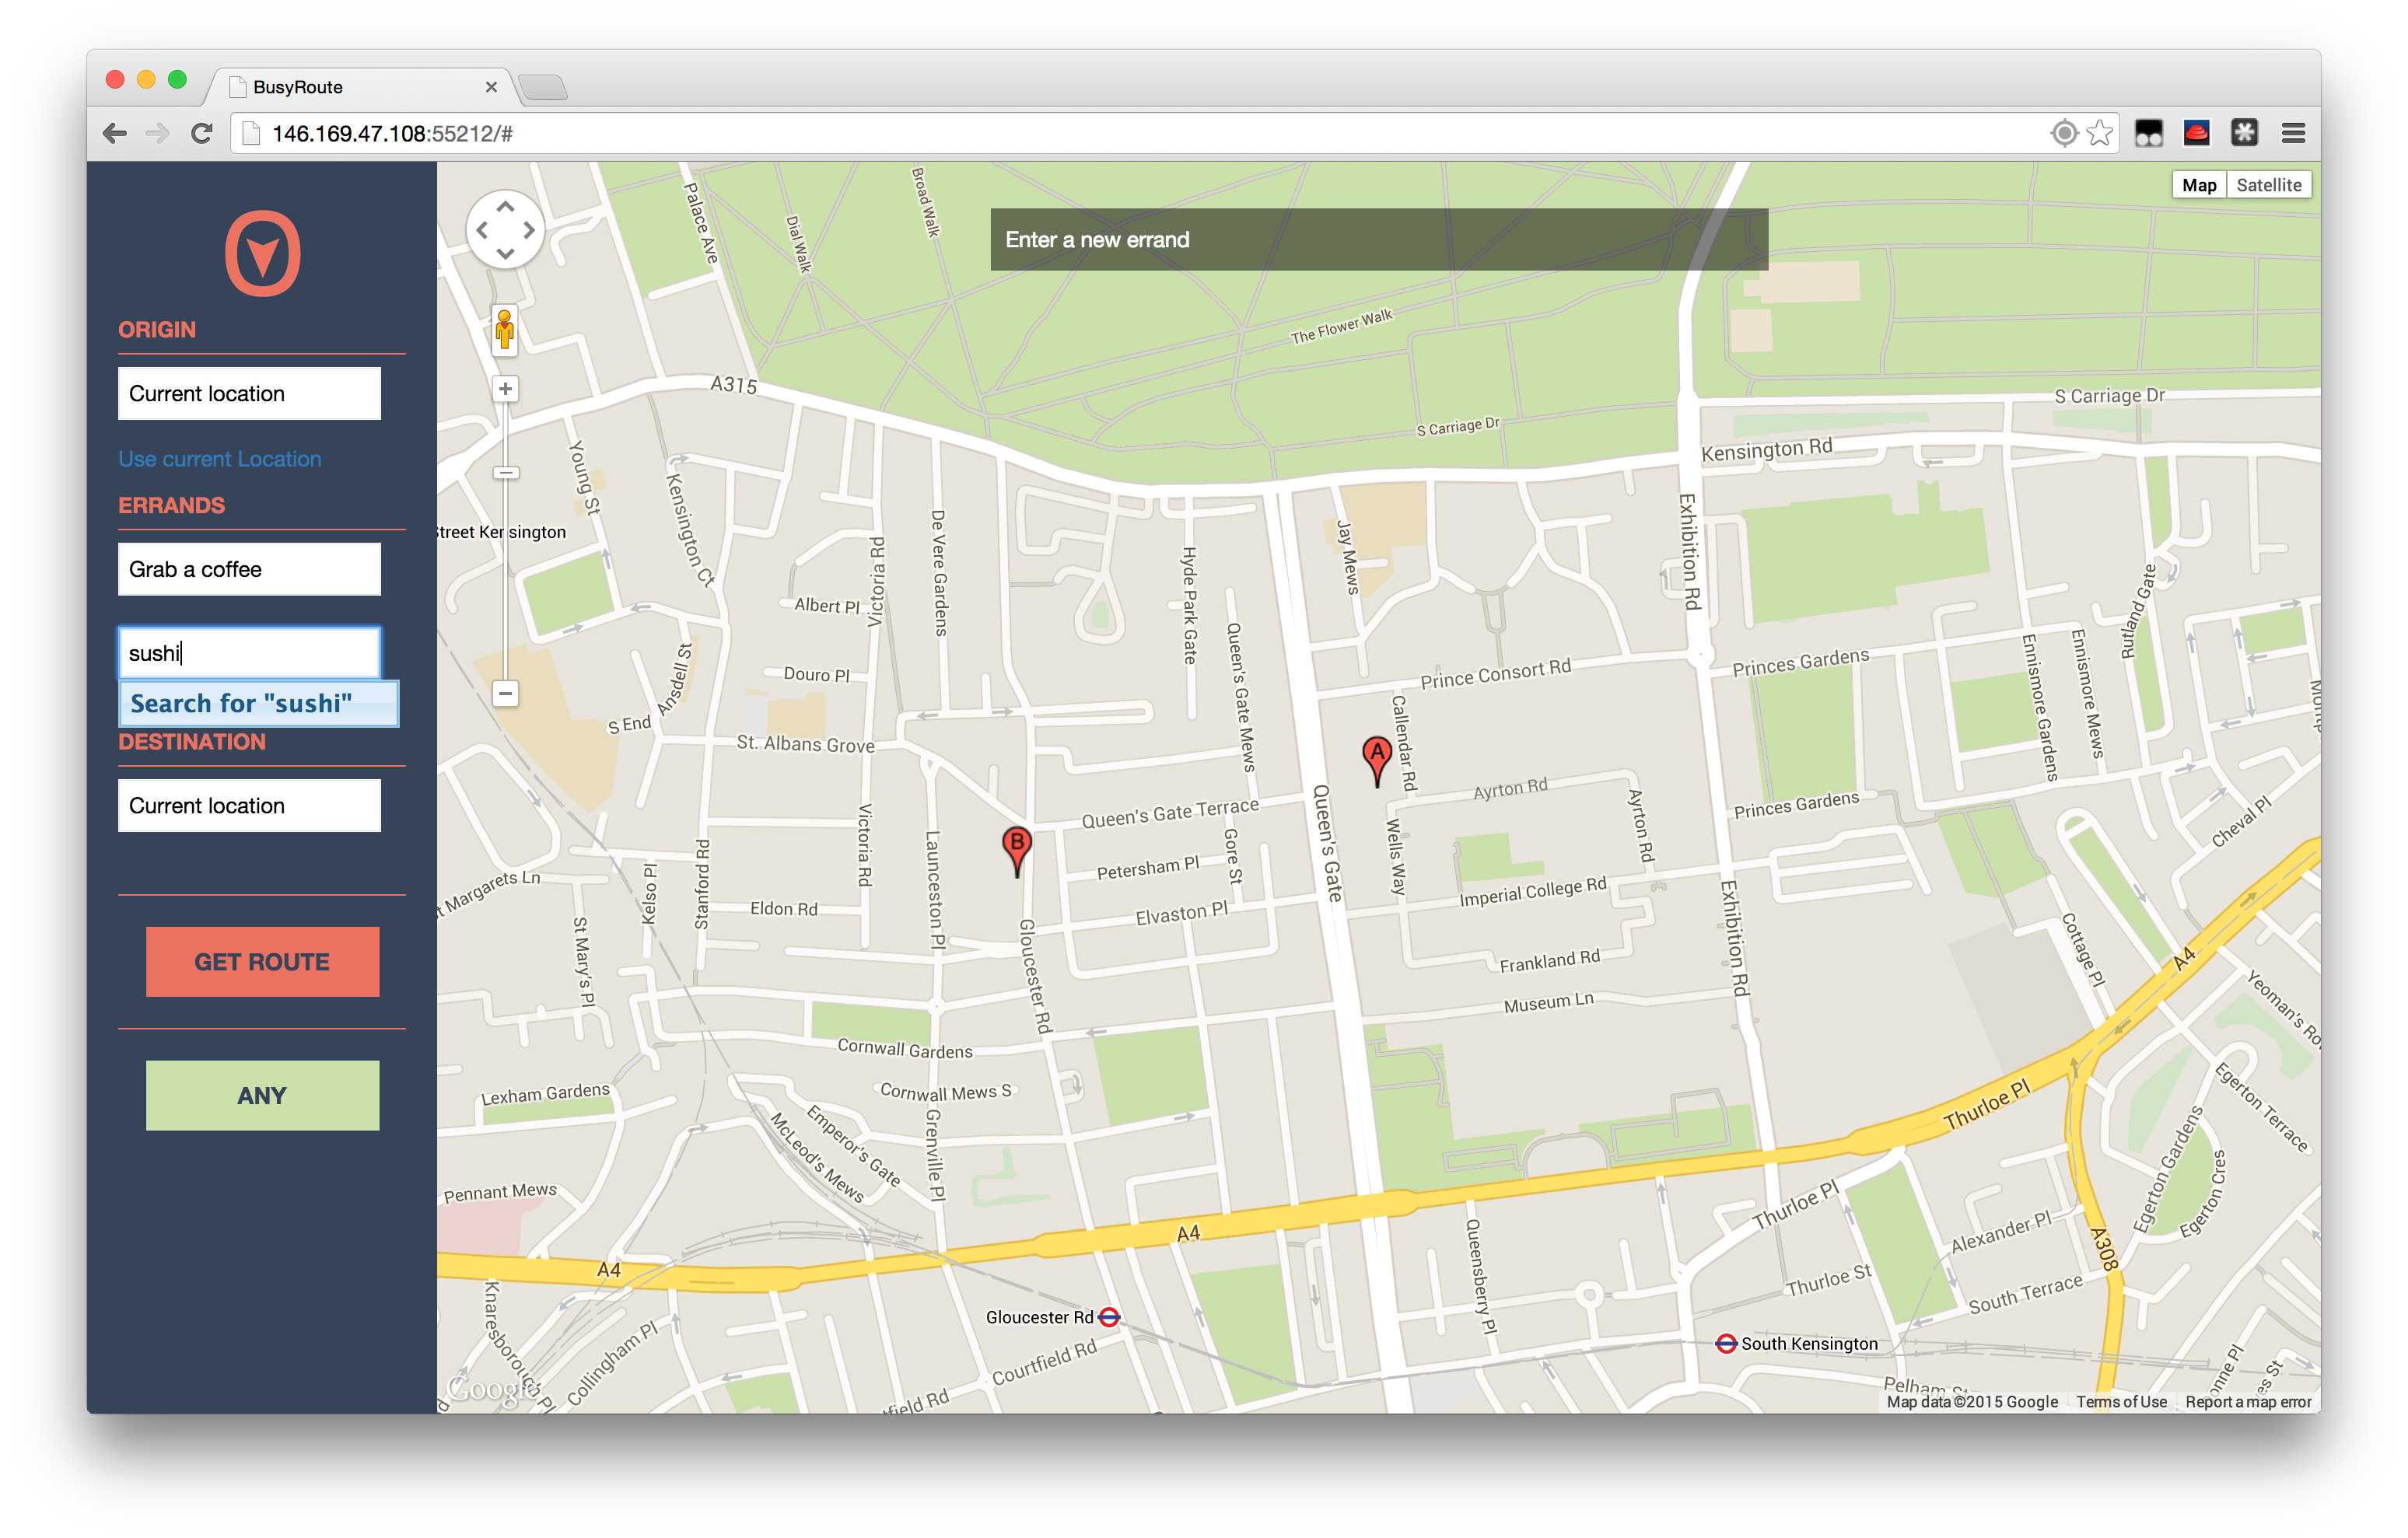
\includegraphics[scale=0.18]{um-07-keyword-search.png}\\
Figure 34. Perform keyword search for non-supported errand.
\end{center}
\begin{center}
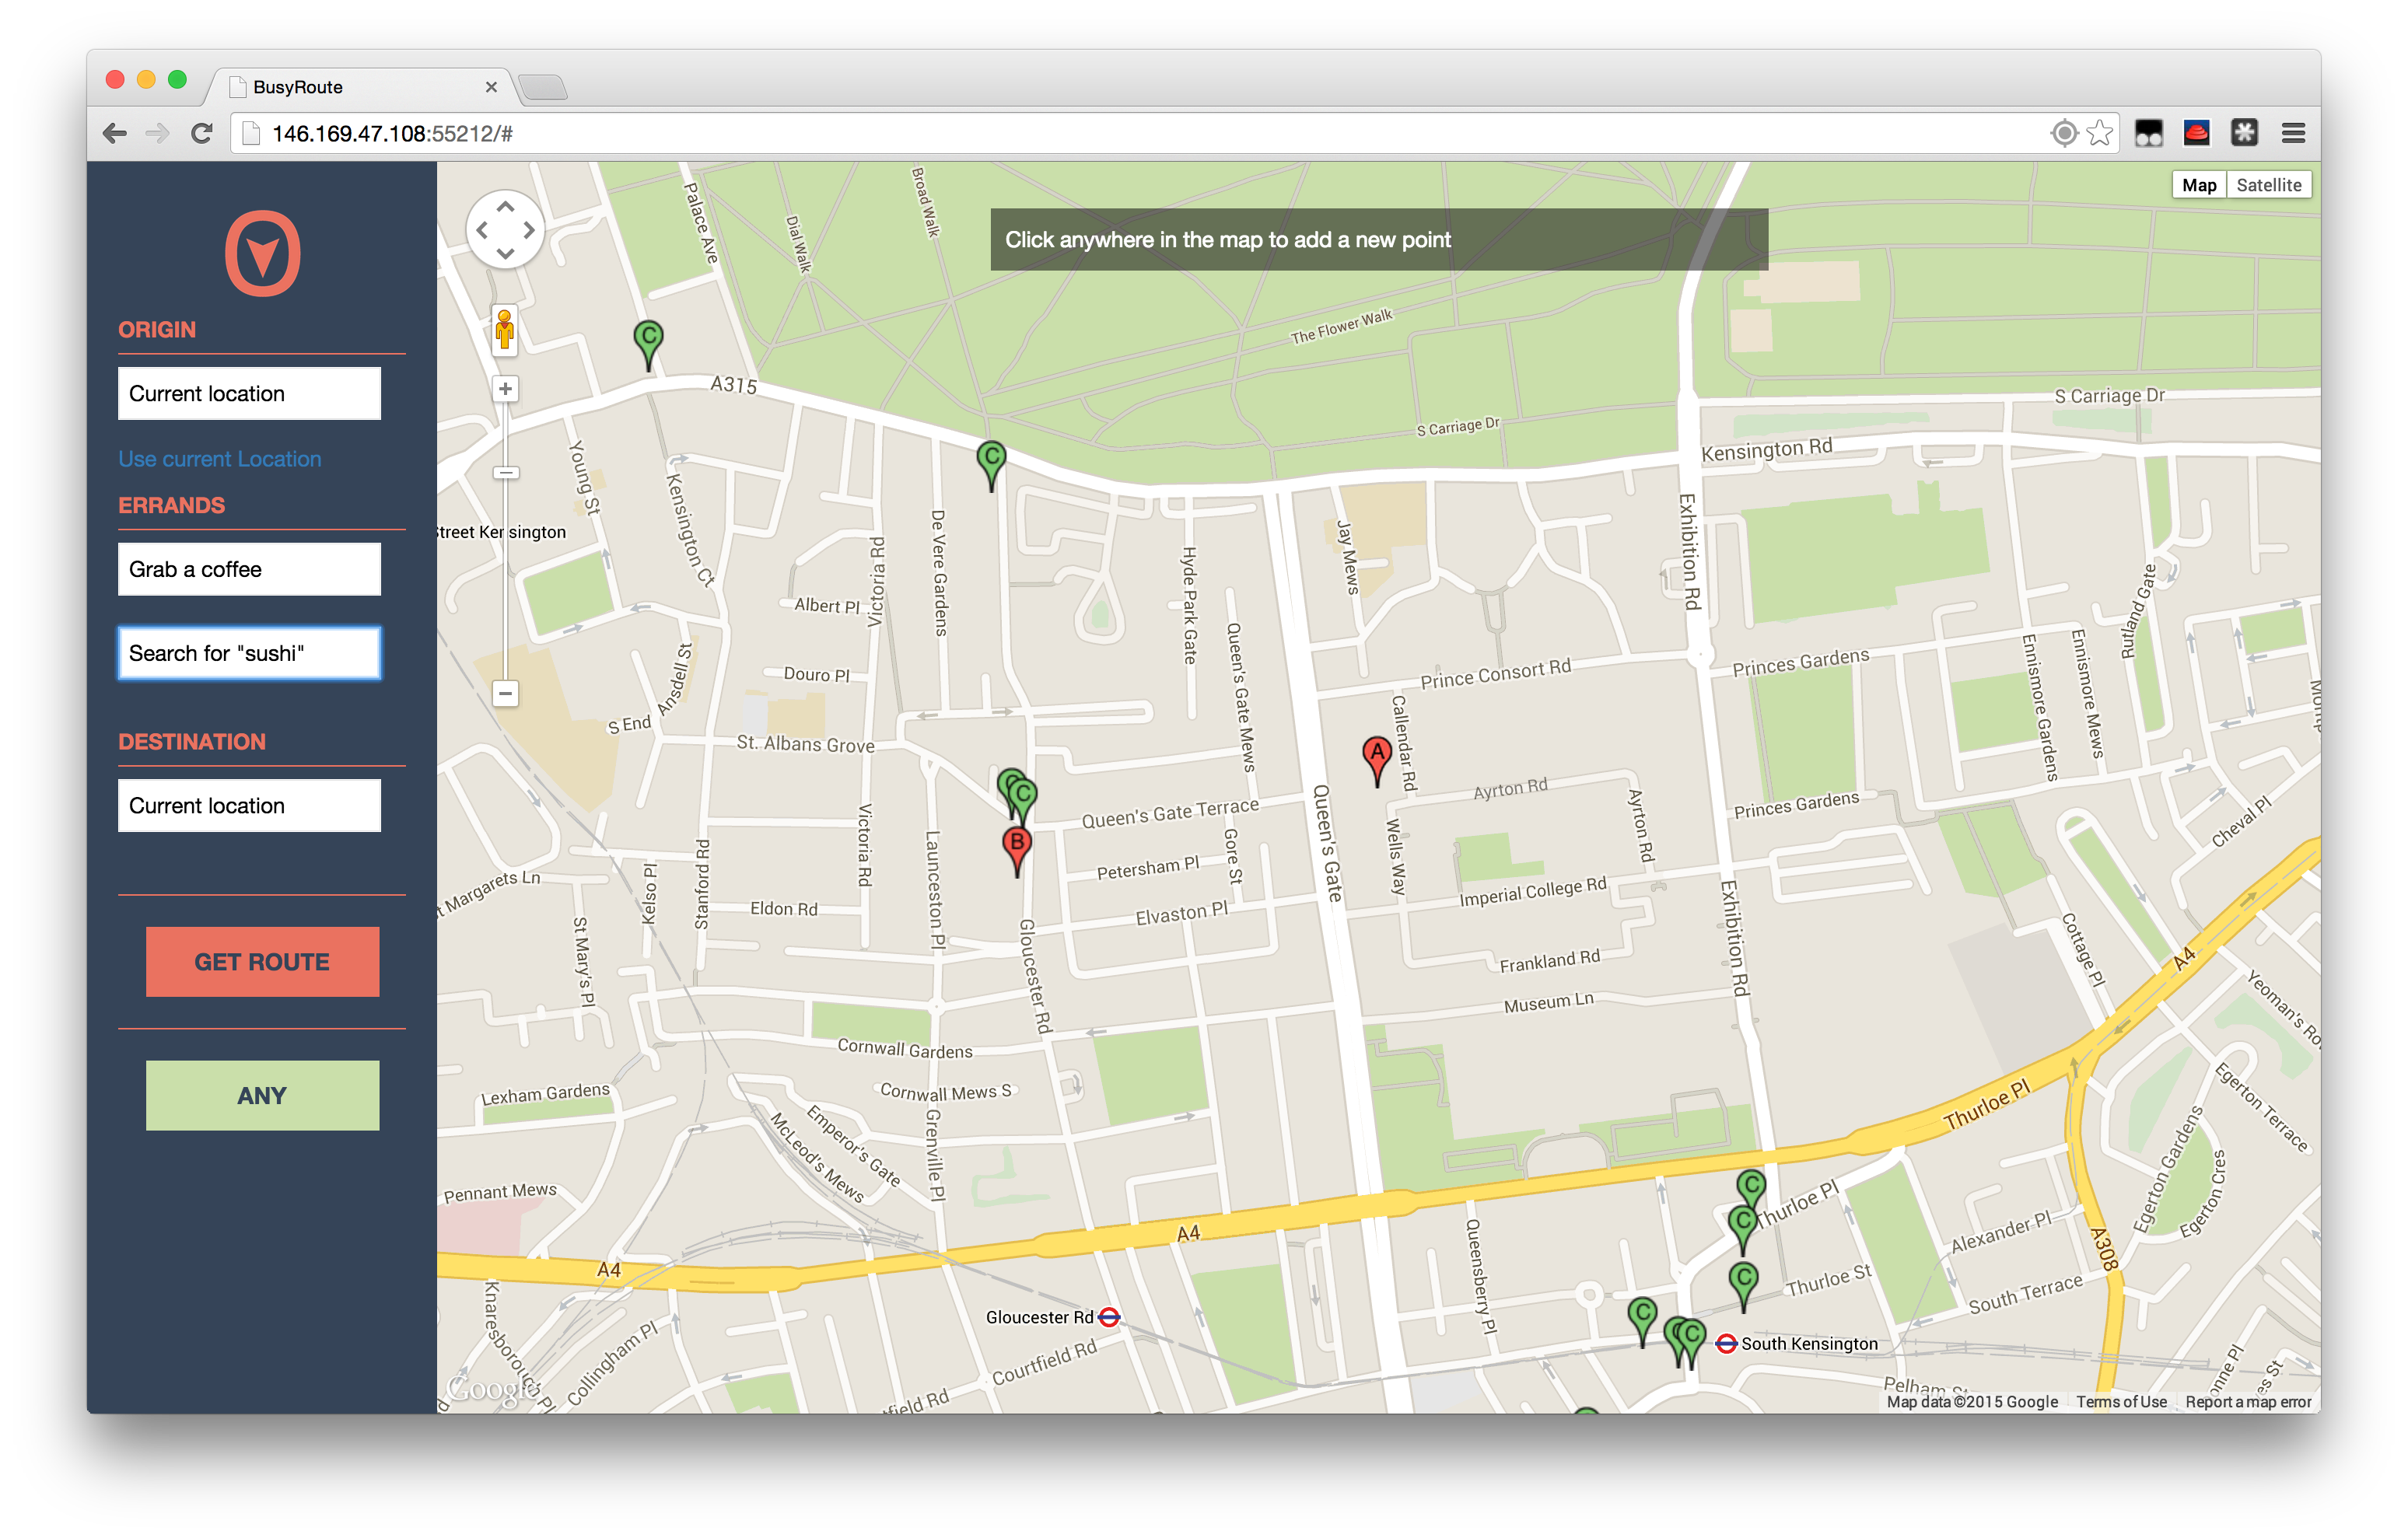
\includegraphics[scale=0.18]{um-08-keyword-results.png}\\
Figure 35. View possible locations for errand completion.
\end{center}
\begin{center}
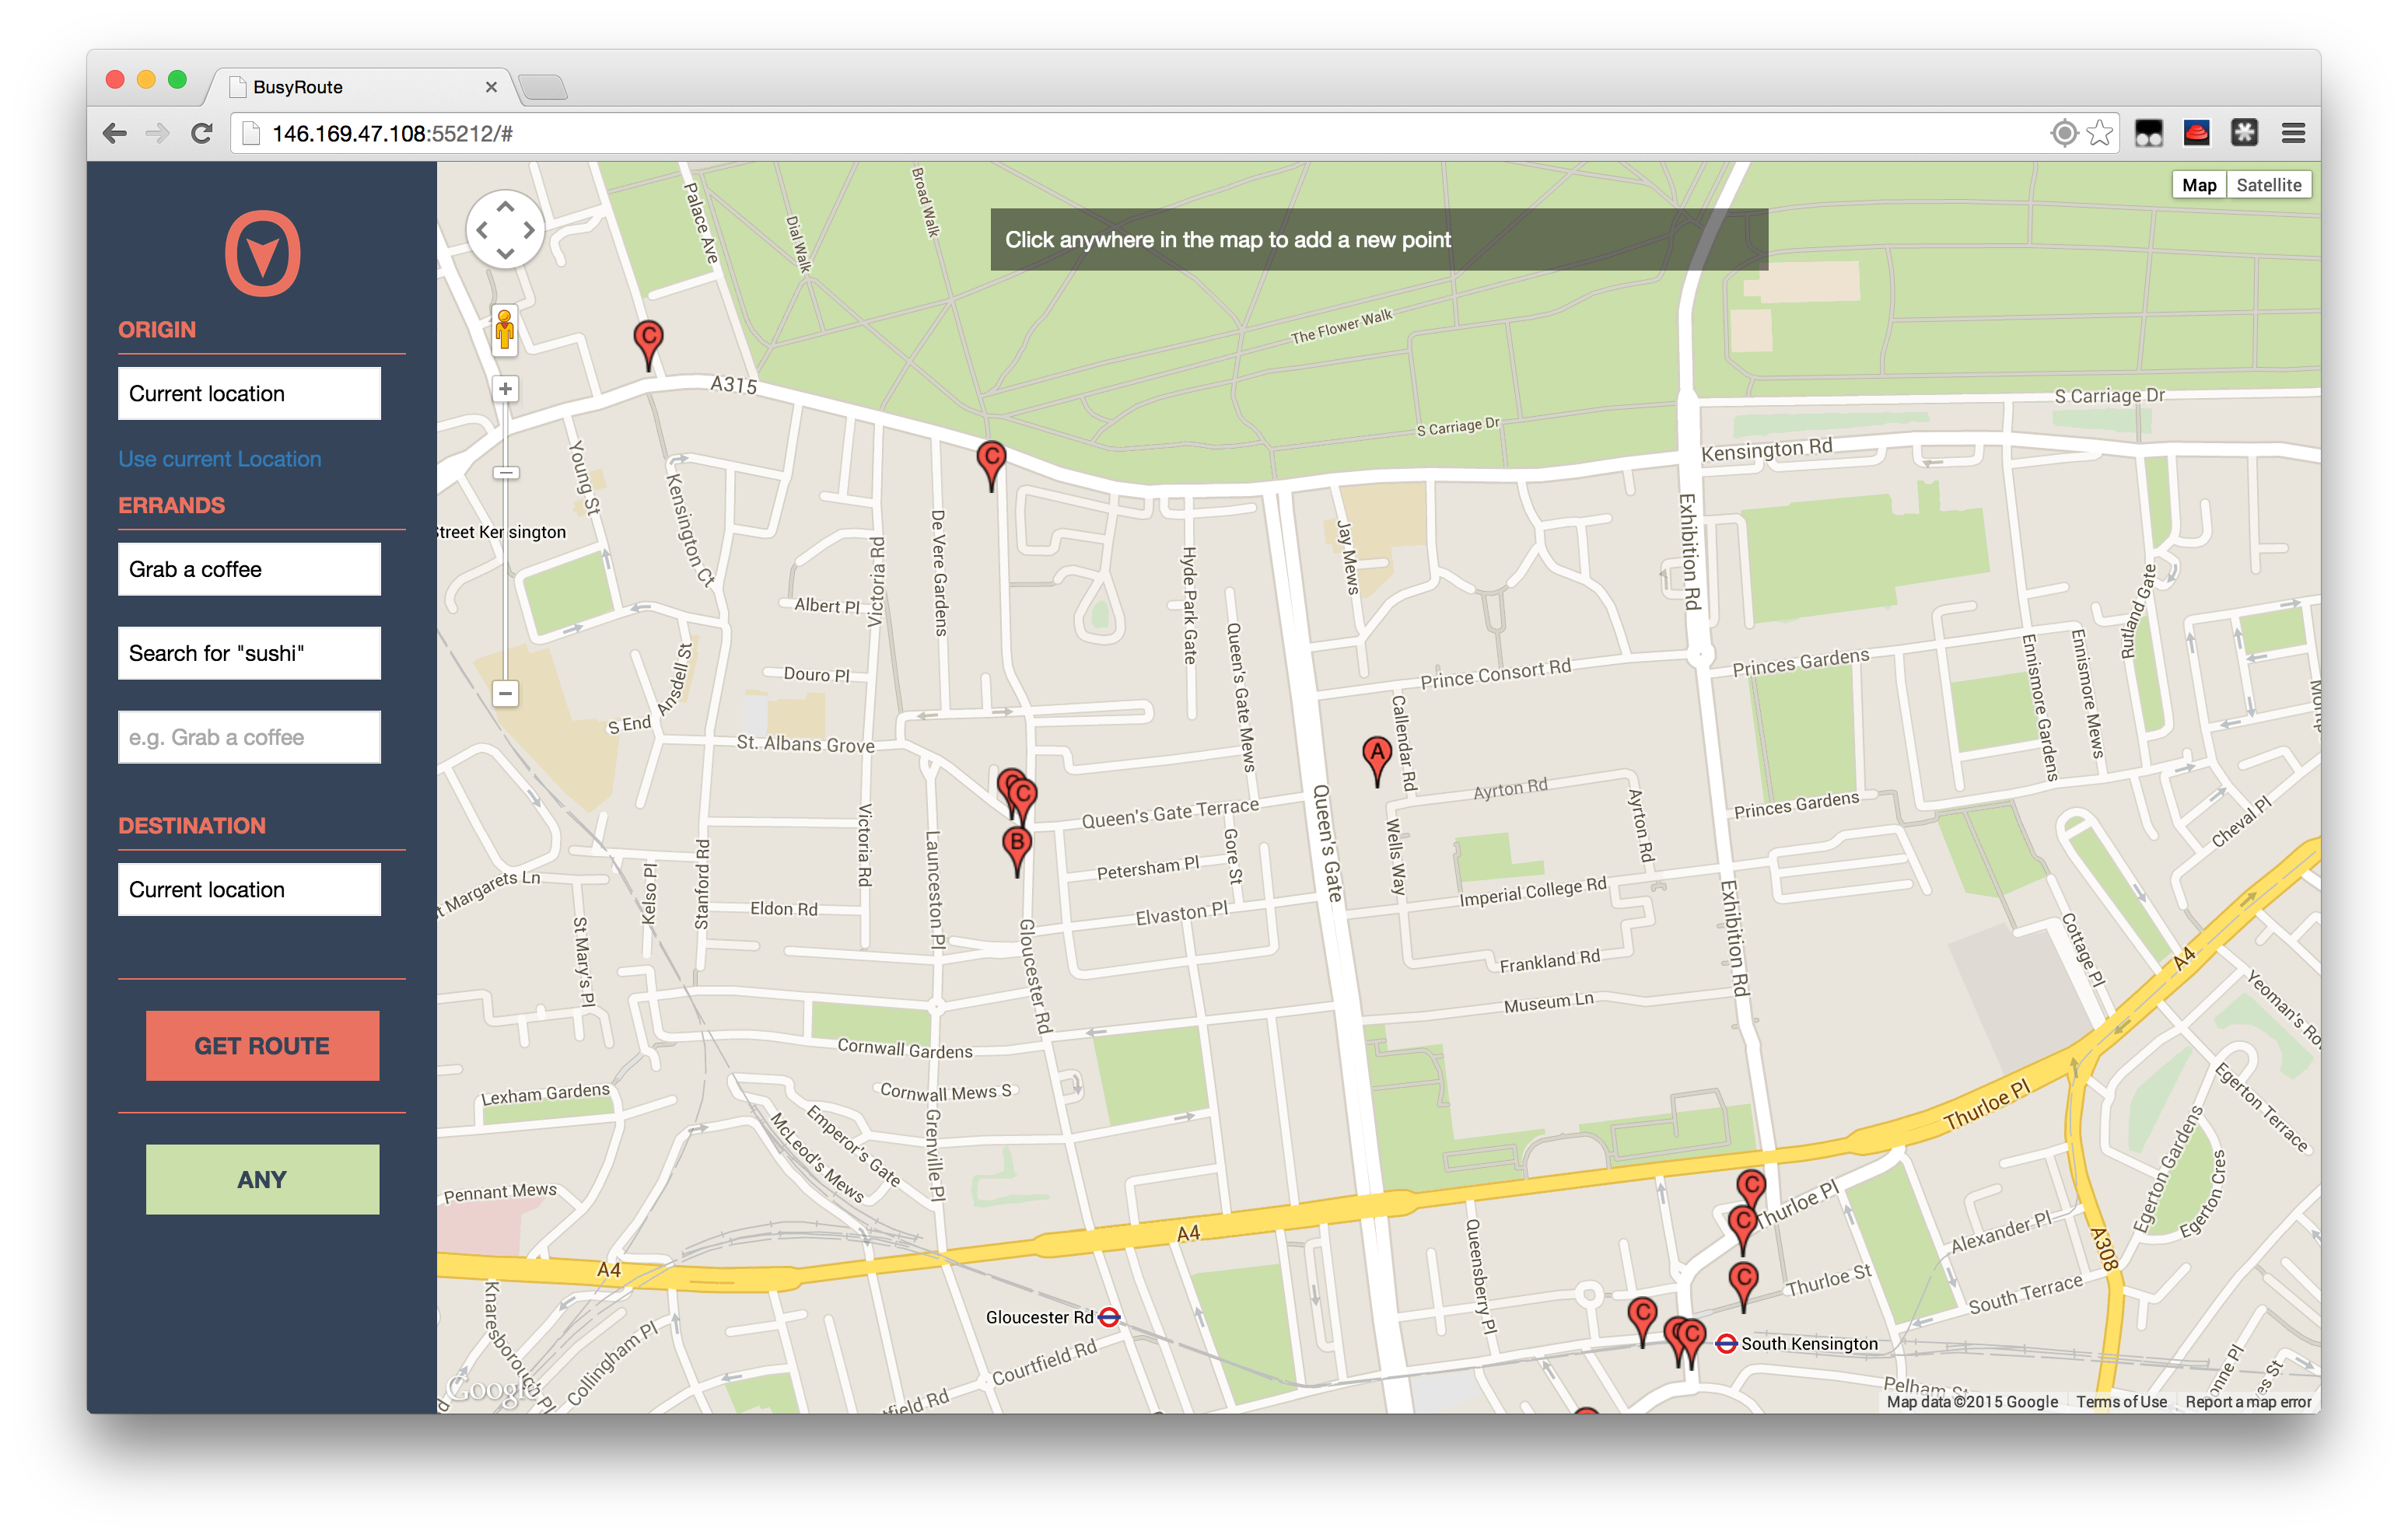
\includegraphics[scale=0.18]{um-09-keyword-any.png}\\
Figure 36. Click ``Any" to express no preference.
\end{center}
\begin{center}
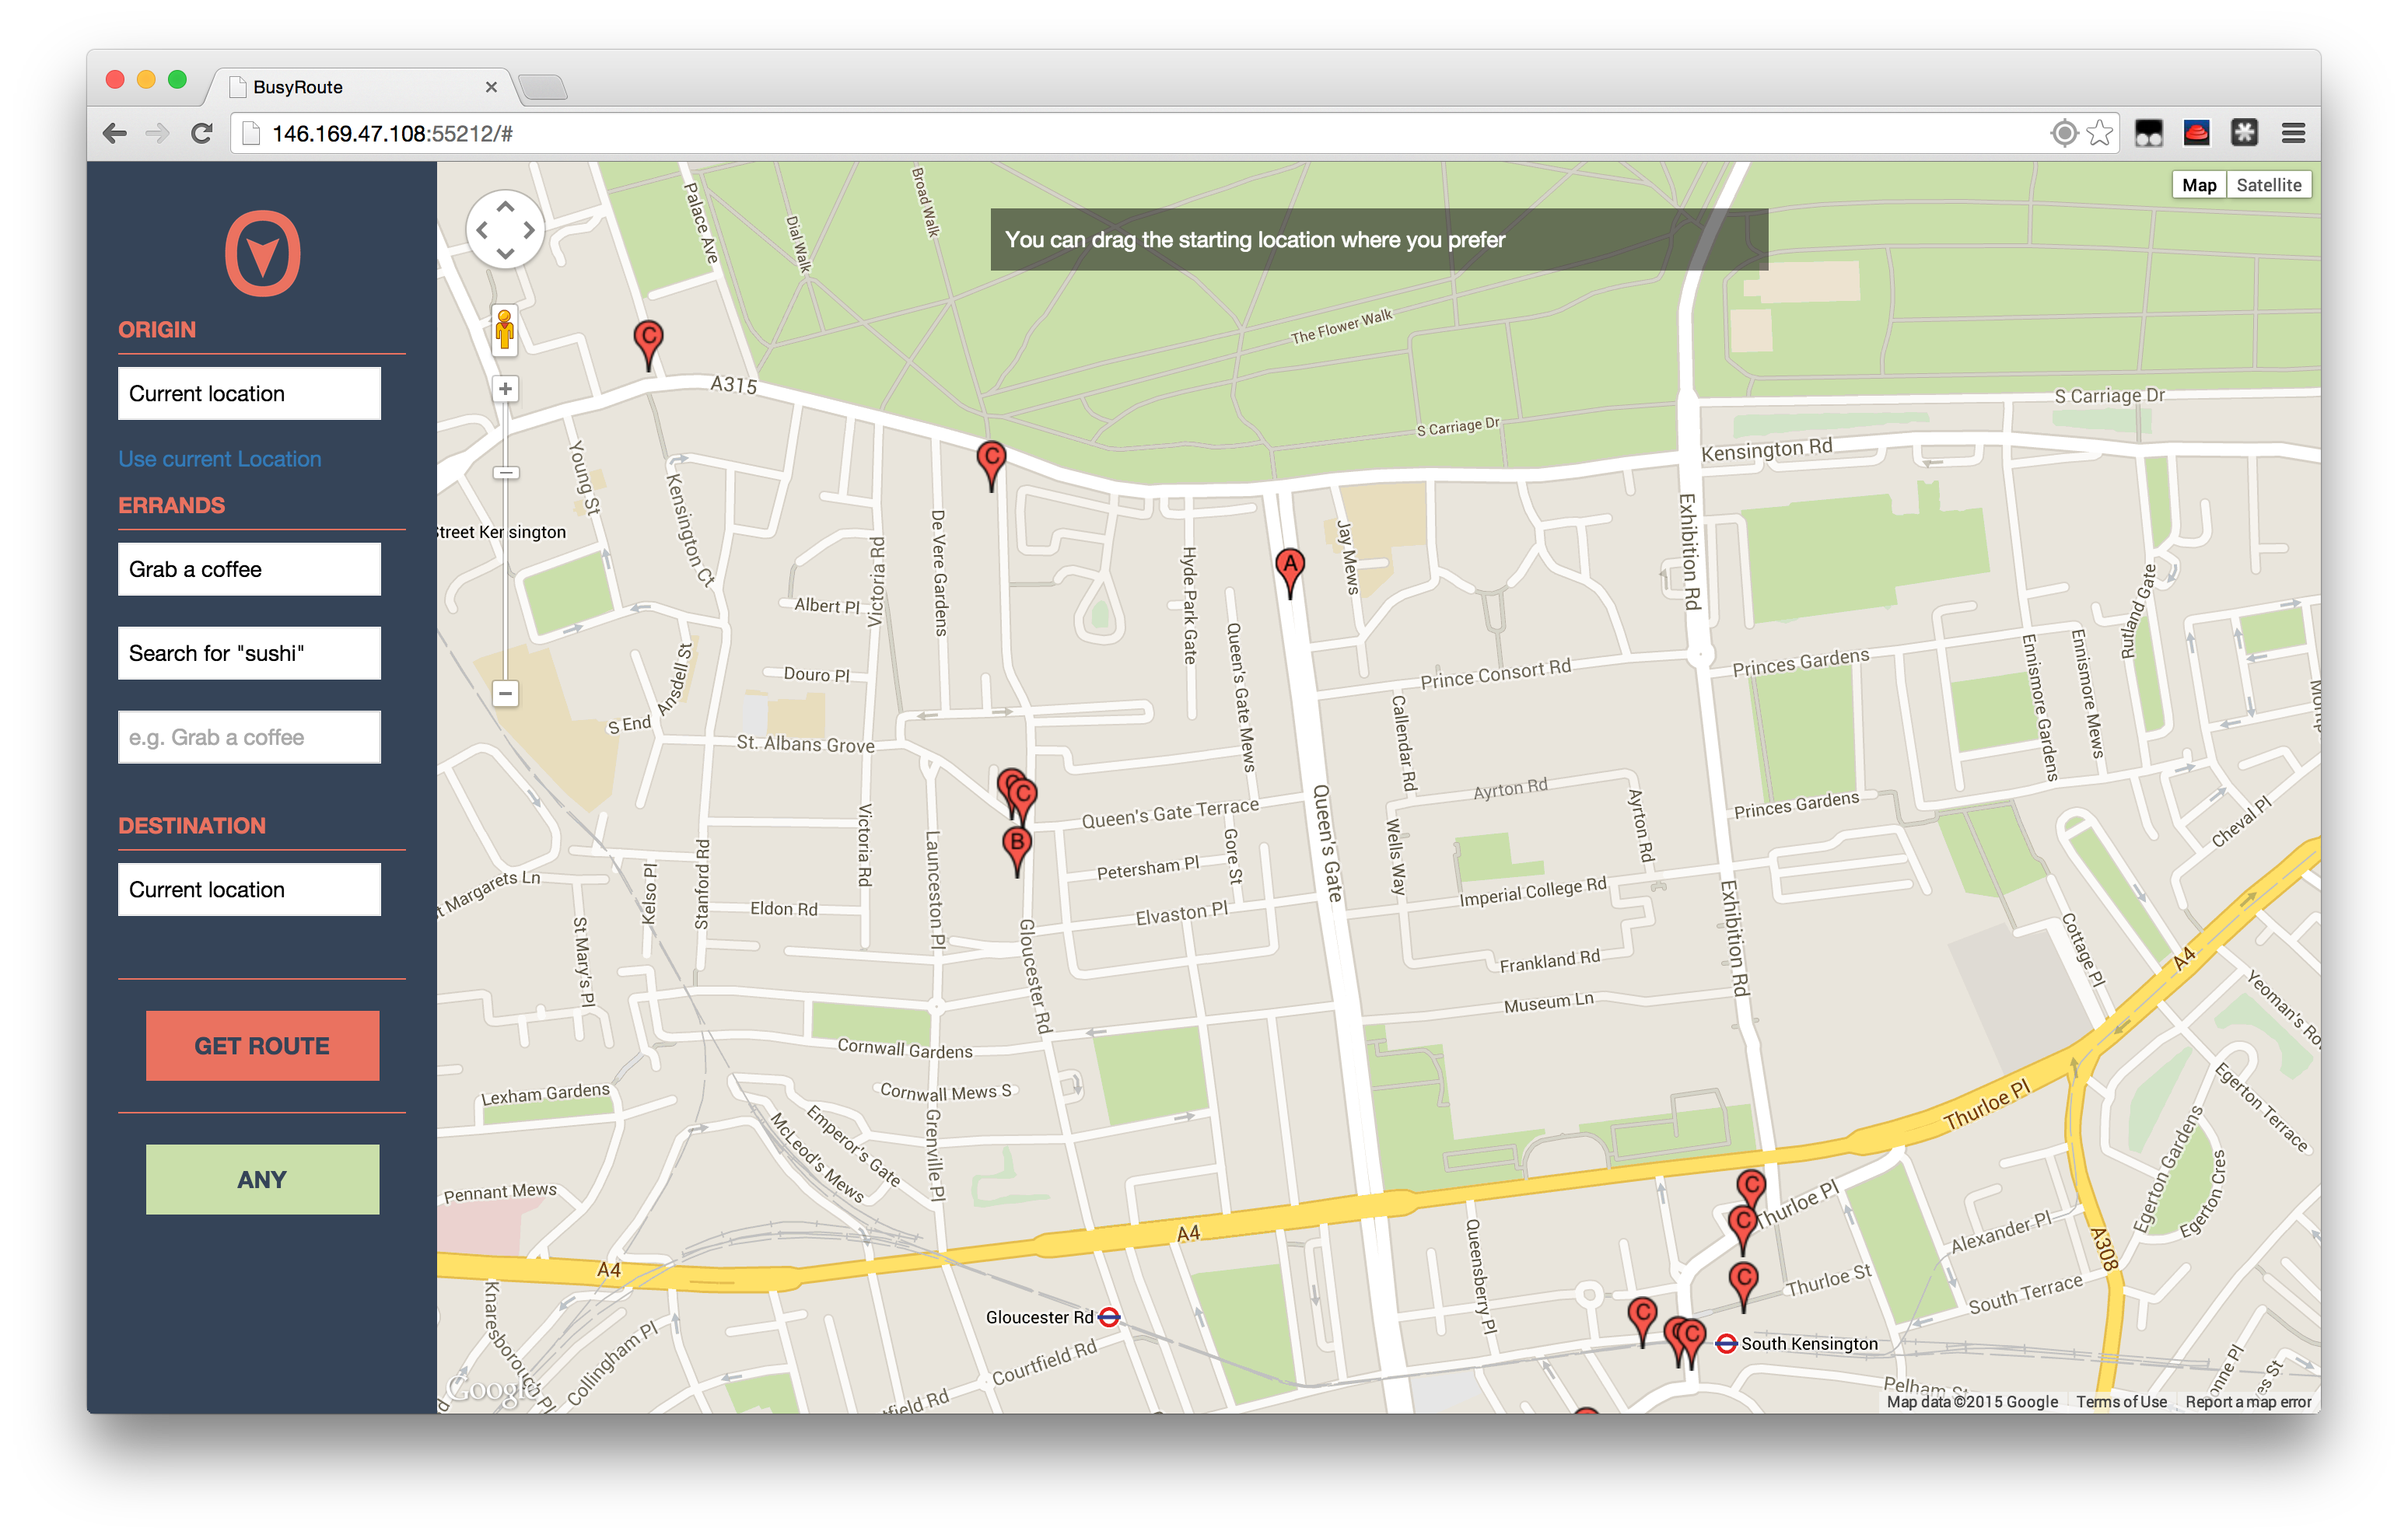
\includegraphics[scale=0.18]{um-10-move-starting.png}\\
Figure 37. Move starting location if required by dragging pin.
\end{center}
\begin{center}
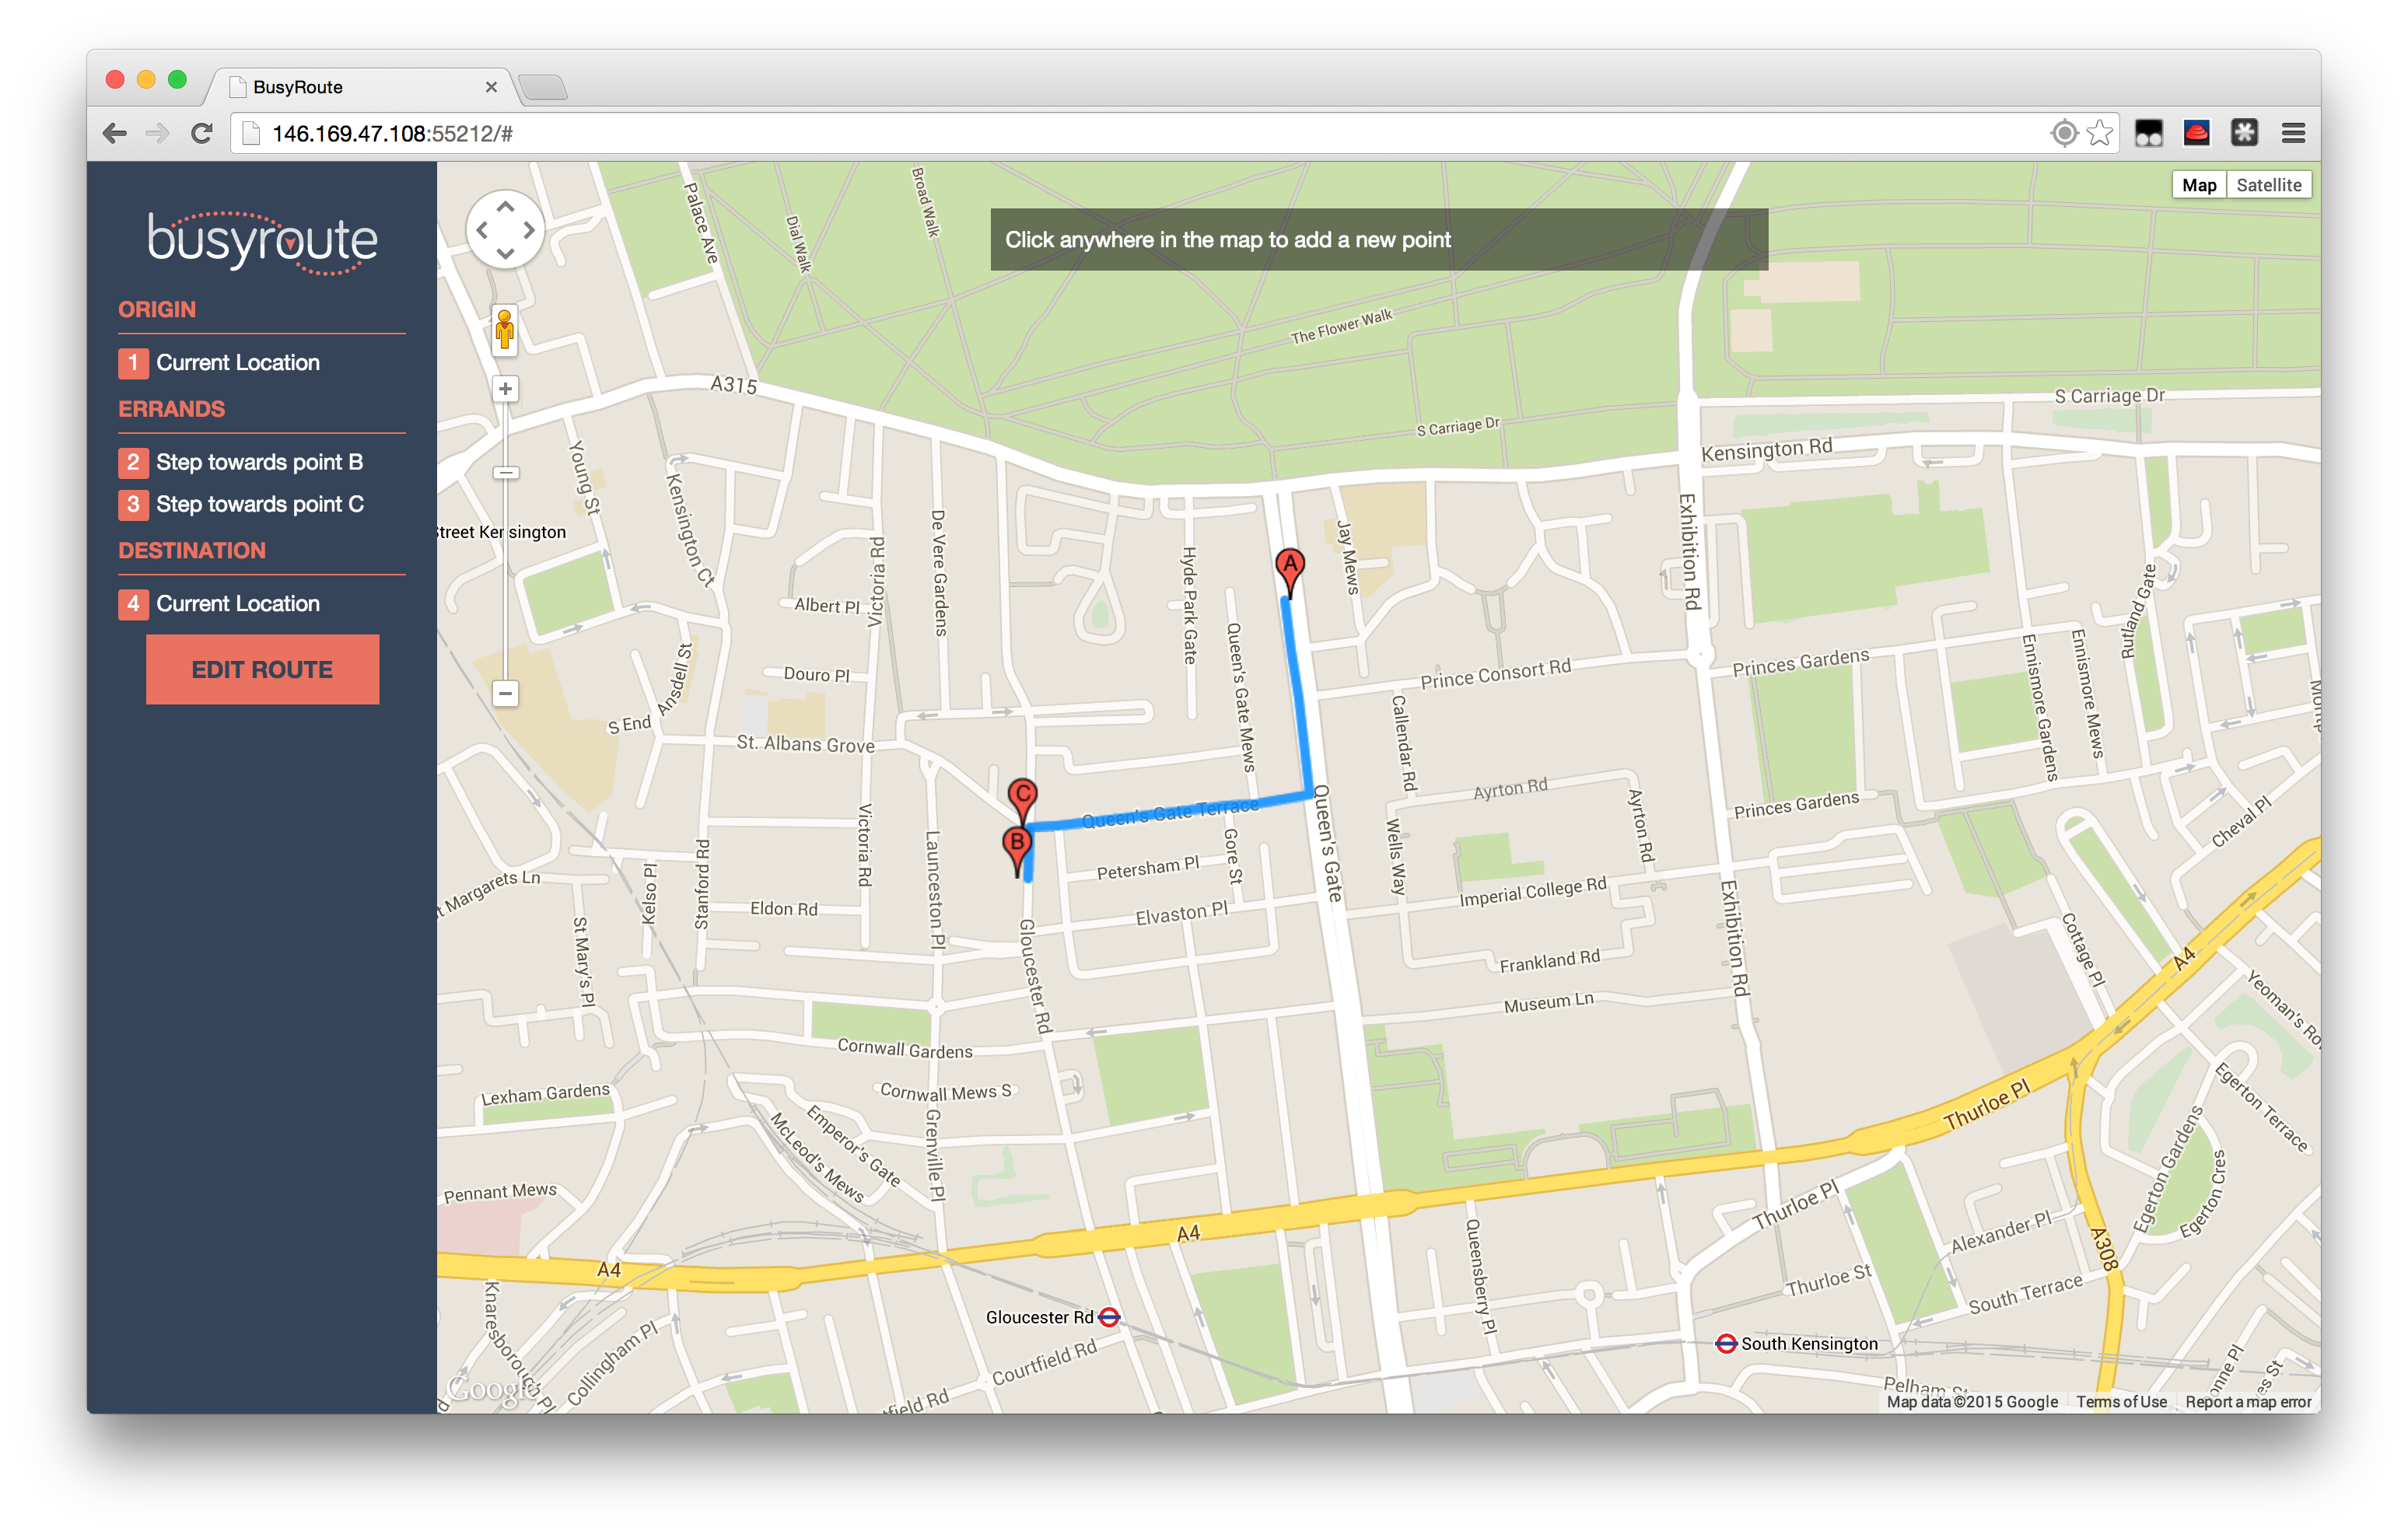
\includegraphics[scale=0.18]{um-11-get-route.png}\\
Figure 38. Click ``Get Route" to find best route.
\end{center}
\begin{center}
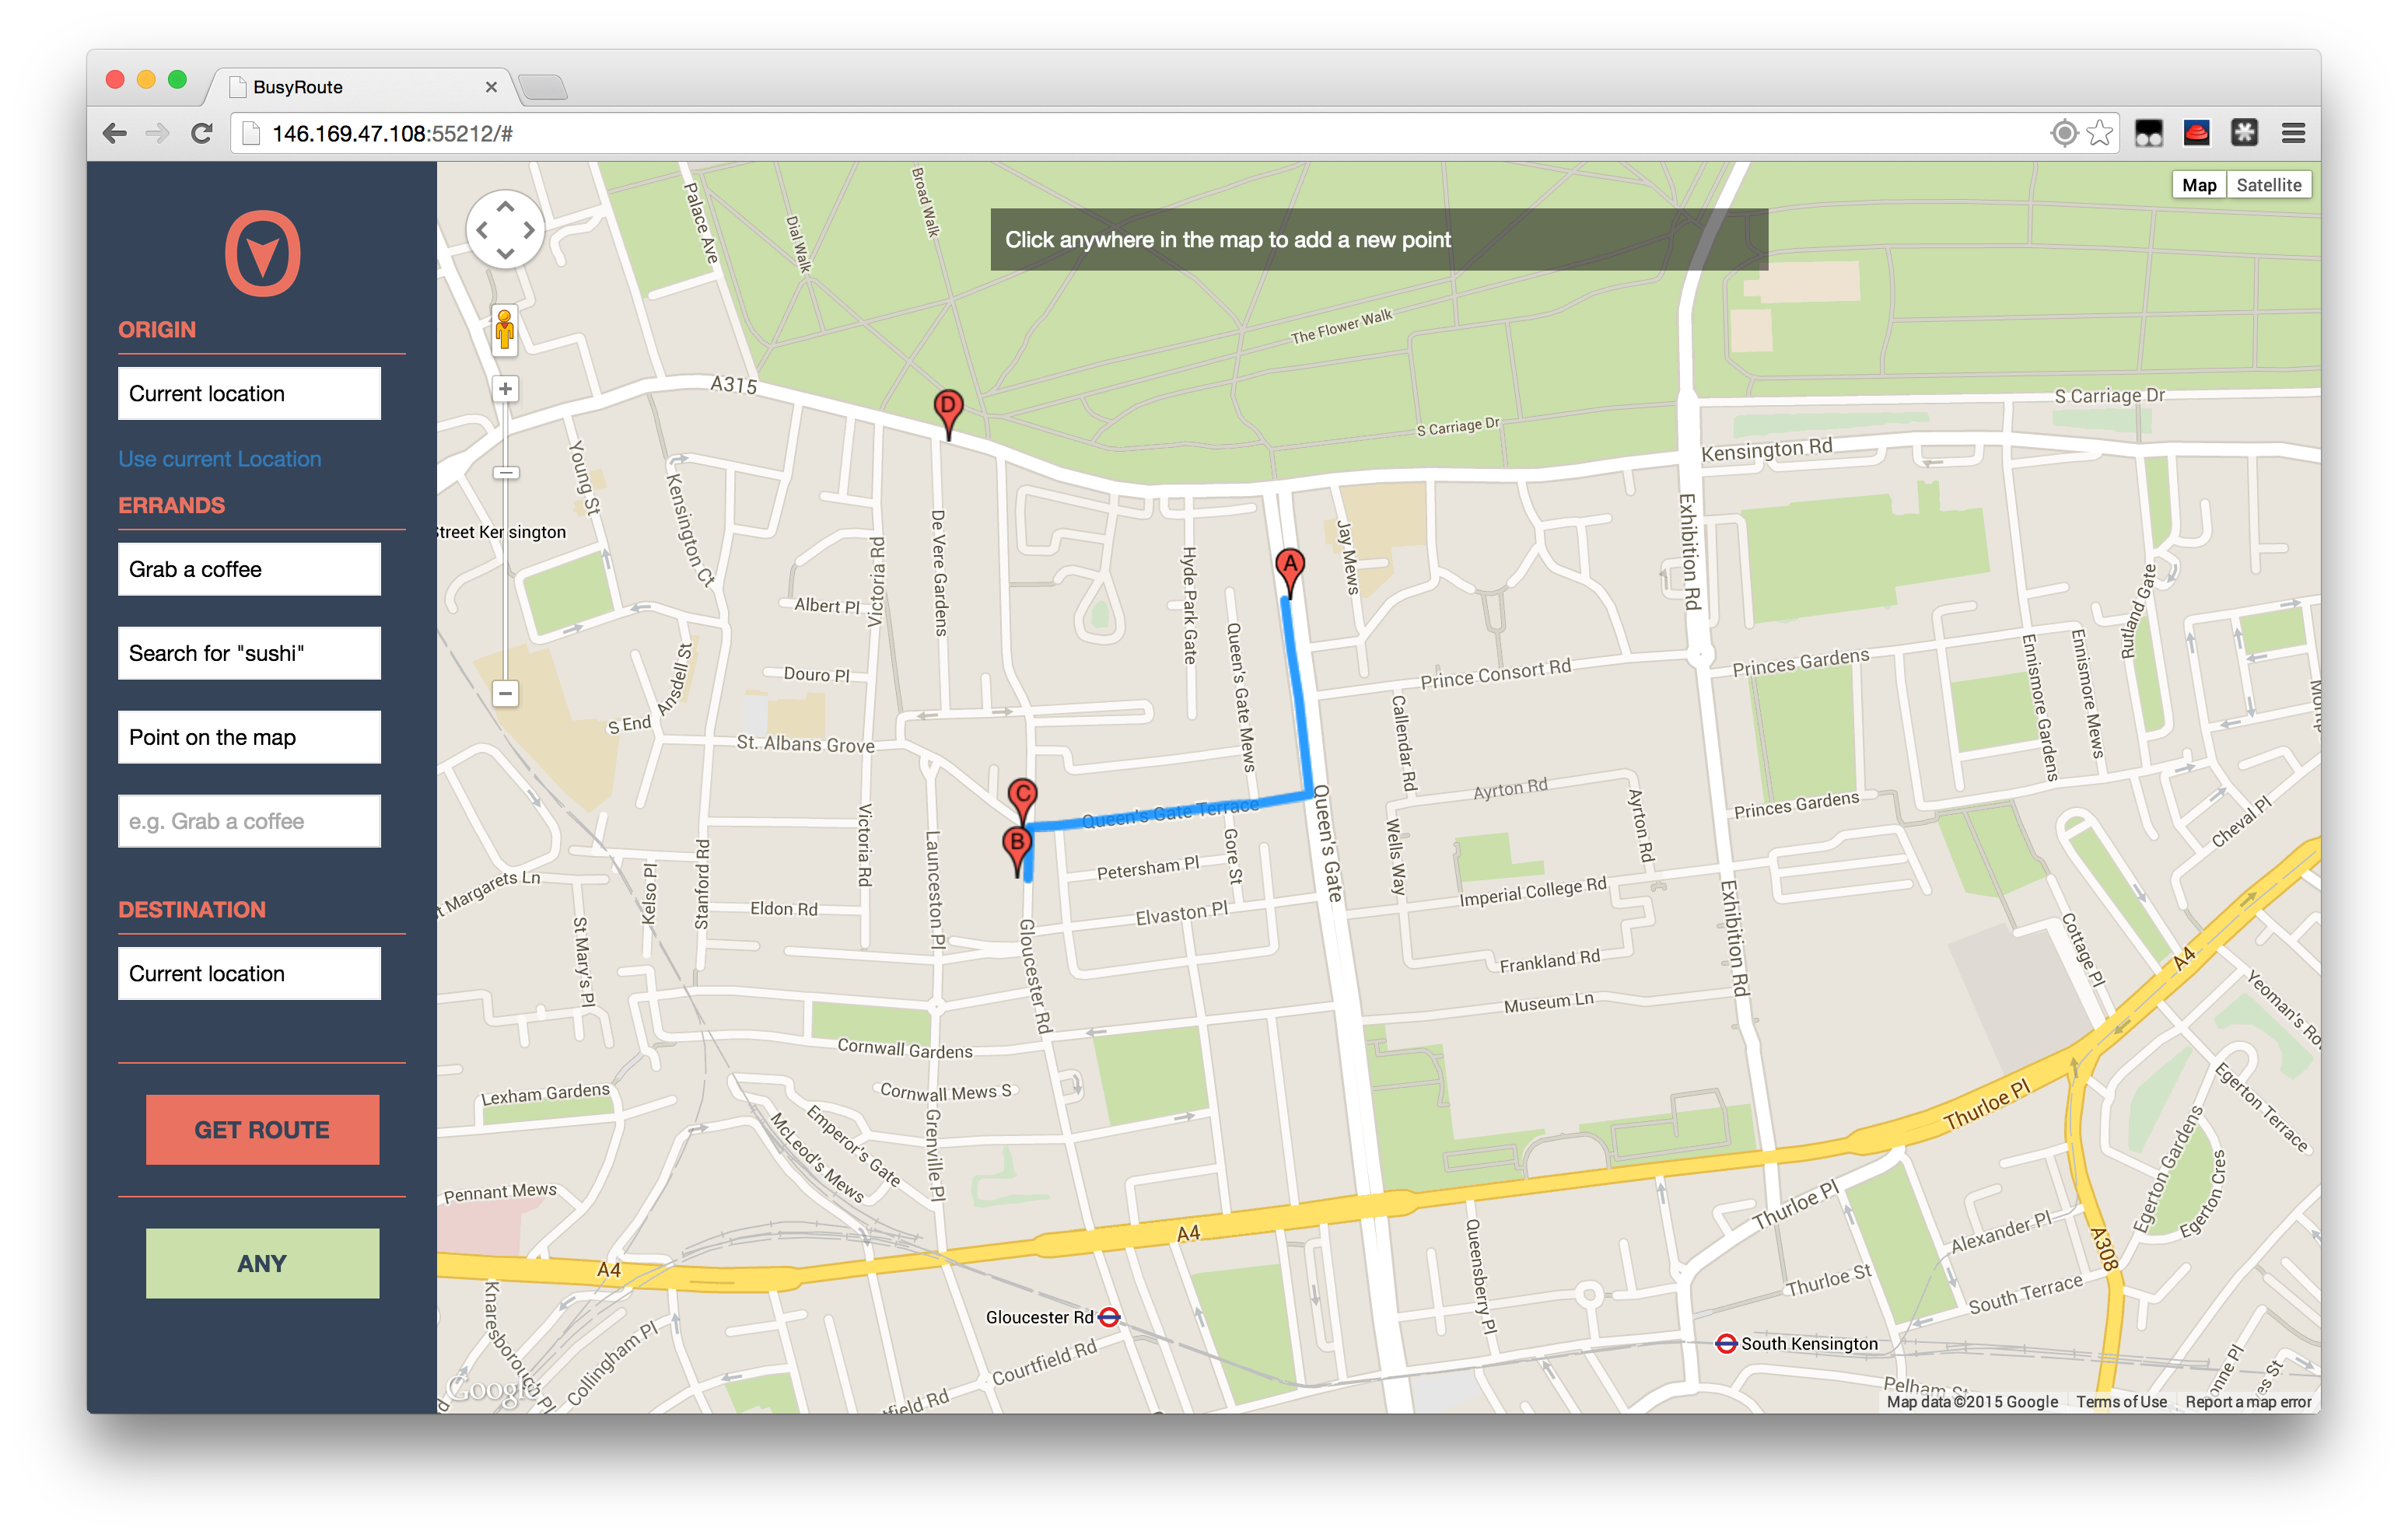
\includegraphics[scale=0.18]{um-12-add-new-point.png}\\
Figure 39. Drop new pins to specify additional locations.
\end{center}
\begin{center}
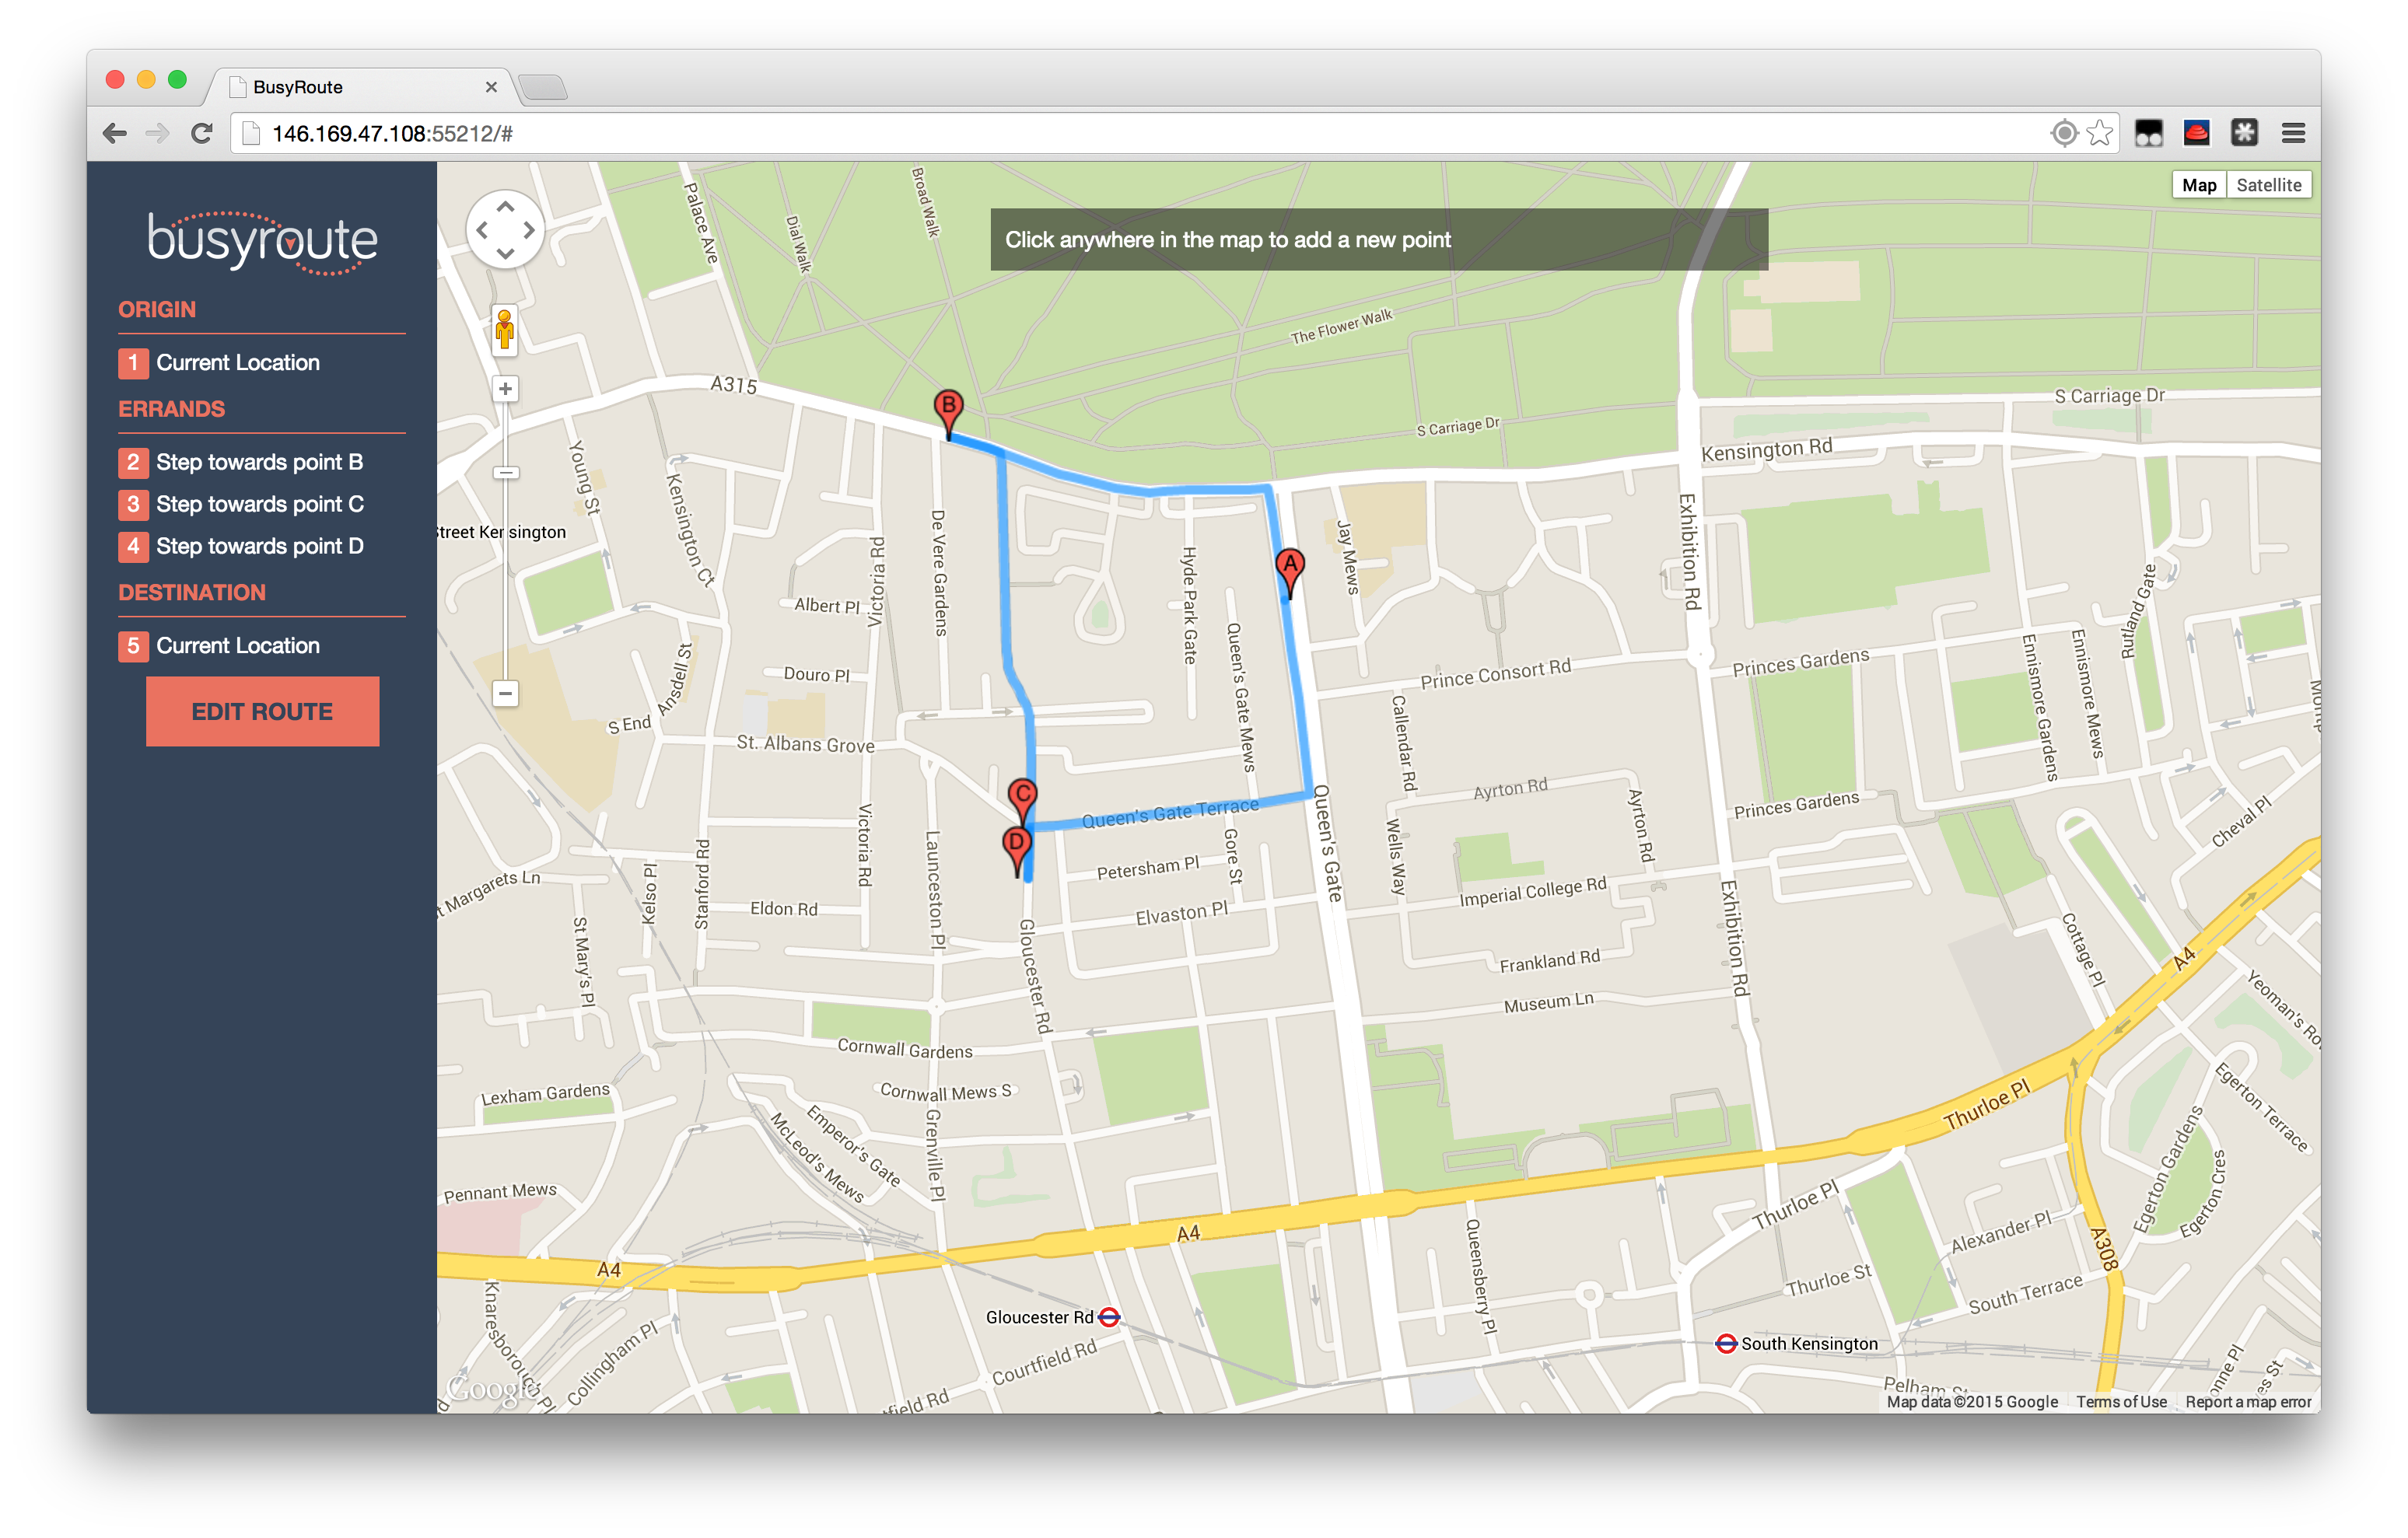
\includegraphics[scale=0.18]{um-13-get-new-route.png}\\
Figure 40. Click ``Get Route" for updated route.
\end{center}

\end{appendices}

\end{document}